\documentclass[12pt, a4paper]{article}



\usepackage{fontspec}
\usepackage{polyglossia}
\usepackage{csquotes}

\setmainlanguage{russian}
\setotherlanguages{english}

% download "Linux Libertine" OTF-fonts:
% http://www.linuxlibertine.org/index.php?id=91&L=1
\setmainfont{Linux Libertine O} % or Helvetica, Arial, Cambria
% why do we need \newfontfamily:
% http://tex.stackexchange.com/questions/91507/
\newfontfamily{\cyrillicfonttt}{Linux Libertine O}
\newfontfamily{\cyrillicfont}{Linux Libertine O}
\newfontfamily{\cyrillicfontsf}{Linux Libertine O}

\usepackage{etoolbox} % to use ifdef, must be after babel


\usepackage[paper=a4paper, top=13.5mm, bottom=13.5mm, left=16.5mm, right=13.5mm, includefoot]{geometry}

\usepackage{etex} % расширение классического tex
% в частности позволяет подгружать гораздо больше пакетов, чем мы и займёмся далее

\usepackage{floatrow} % сильно вниз если сдвинуть - ругается!


\usepackage{makeidx} % для создания предметных указателей
\usepackage{verbatim} % для многострочных комментариев
%\usepackage[pdftex]{graphicx} % для вставки графики
% omit pdftex option if not using pdflatex


%\usepackage{dsfont} % шрифт для единички с двойной палочкой (для индикатора события)
\usepackage{bbm} % шрифт - двойные буквы


\usepackage[usenames, dvipsnames, svgnames, table, rgb]{xcolor}

\usepackage{colortbl}

\usepackage{comment} % для комментирования кусков

% пакет для тестов:
\usepackage[box, % запрет на перенос вопросов
nopage, % убираем колонтитулы страницы
insidebox, % ставим буквы в квадратики
separateanswersheet, % добавляем бланк ответов
nowatermark, % отсутствие надписи "Черновик"
indivanswers,  % показываем верные ответы
%answers,
lang=RU, % локализация слов "нет верных ответов", "вопрос" и тд
completemulti % добавлять "нет правильного ответа" во всех вопросах множественного выбора
]{automultiplechoice}


\usepackage{multicol}
\usepackage{multirow} % Слияние строк в таблице


\usepackage[colorlinks, hyperindex, unicode, breaklinks]{hyperref} % гиперссылки в pdf

\usepackage{dcolumn}

\usepackage{amssymb}
\usepackage{amsmath}
\usepackage{amsthm}
\usepackage{epsfig}
\usepackage{bm}
\usepackage{color}

\usepackage{todonotes} % для вставки в документ заметок о том, что осталось сделать
% \todo{Здесь надо коэффициенты исправить}
% \missingfigure{Здесь будет картина Последний день Помпеи}
% команда \listoftodos — печатает все поставленные \todo'шки


\usepackage{textcomp}  % Чтобы в формулах можно было русские буквы писать через \text{}

%\usepackage{embedfile} % Чтобы код LaTeXа включился как приложение в PDF-файл

\usepackage{subfigure} % для создания нескольких рисунков внутри одного

\usepackage{tikz, pgfplots} % язык для рисования графики из latex'a
\usetikzlibrary{trees} % прибамбас в нем для рисовки деревьев
\usetikzlibrary{arrows} % прибамбас в нем для рисовки стрелочек подлиннее
\usepackage{tikz-qtree} % прибамбас в нем для рисовки деревьев




\usepackage{enumitem}


%\embedfile[desc={Исходный LaTeX файл}]{\jobname.tex} % Включение кода в выходной файл
%\embedfile[desc={Стилевой файл}]{title_bor_utf8.tex}



% вместо горизонтальной делаем косую черточку в нестрогих неравенствах
\renewcommand{\le}{\leqslant}
\renewcommand{\ge}{\geqslant}
\renewcommand{\leq}{\leqslant}
\renewcommand{\geq}{\geqslant}

% делаем короче интервал в списках
\setlength{\itemsep}{0pt}
\setlength{\parskip}{0pt}
\setlength{\parsep}{0pt}

% свешиваем пунктуацию (т.е. знаки пунктуации могут вылезать за правую границу текста, при этом текст выглядит ровнее)
\usepackage{microtype}

% более красивые таблицы
\usepackage{booktabs}
% заповеди из докупентации:
% 1. Не используйте вертикальные линни
% 2. Не используйте двойные линии
% 3. Единицы измерения - в шапку таблицы
% 4. Не сокращайте .1 вместо 0.1
% 5. Повторяющееся значение повторяйте, а не говорите "то же"


% DEFS
\def \mbf{\mathbf}
\def \msf{\mathsf}
\def \mbb{\mathbb}
\def \tbf{\textbf}
\def \tsf{\textsf}
\def \ttt{\texttt}
\def \tbb{\textbb}

\def \wh{\widehat}
\def \wt{\widetilde}
\def \ni{\noindent}
\def \ol{\overline}
\def \cd{\cdot}
\def \bl{\bigl}
\def \br{\bigr}
\def \Bl{\Bigl}
\def \Br{\Bigr}
\def \fr{\frac}
\def \bs{\backslash}
\def \lims{\limits}
\def \arg{{\operatorname{arg}}}
\def \dist{{\operatorname{dist}}}
\def \VC{{\operatorname{VCdim}}}
\def \card{{\operatorname{card}}}
\def \sgn{{\operatorname{sign}\,}}
\def \sign{{\operatorname{sign}\,}}
\def \xfs{(x_1,\ldots,x_{n-1})}
\def \Tr{{\operatorname{\mbf{Tr}}}}
\DeclareMathOperator*{\argmin}{arg\,min}
\DeclareMathOperator*{\argmax}{arg\,max}
\DeclareMathOperator*{\amn}{arg\,min}
\DeclareMathOperator*{\amx}{arg\,max}
\def \cov{{\operatorname{Cov}}}
\DeclareMathOperator{\Var}{Var}
\DeclareMathOperator{\Cov}{Cov}
\DeclareMathOperator{\Corr}{Corr}
\DeclareMathOperator{\grad}{grad}
\DeclareMathOperator{\trace}{trace}
\DeclareMathOperator{\rank}{rank}

\def \xfs{(x_1,\ldots,x_{n-1})}
\def \ti{\tilde}
\def \wti{\widetilde}


\def \mL{\mathcal{L}}
\def \mW{\mathcal{W}}
\def \mH{\mathcal{H}}
\def \mC{\mathcal{C}}
\def \mE{\mathcal{E}}
\def \mN{\mathcal{N}}
\def \mA{\mathcal{A}}
\def \mB{\mathcal{B}}
\def \mU{\mathcal{U}}
\def \mV{\mathcal{V}}
\def \mF{\mathcal{F}}

\def \R{\mbb R}
\def \N{\mbb N}
\def \Z{\mbb Z}
\def \P{\mbb{P}}
%\def \p{\mbb{P}}
\def \E{\mbb{E}}
\def \D{\msf{D}}
\def \I{\mbf{I}}

\def \a{\alpha}
\def \b{\beta}
\def \t{\tau}
\def \dt{\delta}
\def \e{\varepsilon}
\def \ga{\gamma}
\def \kp{\varkappa}
\def \la{\lambda}
\def \sg{\sigma}
\def \sgm{\sigma}
\def \tt{\theta}
\def \ve{\varepsilon}
\def \Dt{\Delta}
\def \La{\Lambda}
\def \Sgm{\Sigma}
\def \Sg{\Sigma}
\def \Tt{\Theta}
\def \Om{\Omega}
\def \om{\omega}


\def \ni{\noindent}
\def \lq{\glqq}
\def \rq{\grqq}
\def \lbr{\linebreak}
\def \vsi{\vspace{0.1cm}}
\def \vsii{\vspace{0.2cm}}
\def \vsiii{\vspace{0.3cm}}
\def \vsiv{\vspace{0.4cm}}
\def \vsv{\vspace{0.5cm}}
\def \vsvi{\vspace{0.6cm}}
\def \vsvii{\vspace{0.7cm}}
\def \vsviii{\vspace{0.8cm}}
\def \vsix{\vspace{0.9cm}}
\def \VSI{\vspace{1cm}}
\def \VSII{\vspace{2cm}}
\def \VSIII{\vspace{3cm}}



\newcommand{\dx}[1]{\,\mathrm{d}#1} % для интеграла: маленький отступ и прямая d
\newcommand{\ind}[1]{\mathbbm{1}_{\{#1\}}} % Индикатор события
%\renewcommand{\to}{\rightarrow}
\newcommand{\eqdef}{\mathrel{\stackrel{\rm def}=}}
\newcommand{\iid}{\mathrel{\stackrel{\rm i.\,i.\,d.}\sim}}
\newcommand{\const}{\mathrm{const}}

%на всякий случай пока есть
%теоремы без нумерации и имени
\newtheorem*{theorem}{Теорема}

%"Определения","Замечания"
%и "Гипотезы" не нумеруются
\newtheorem*{definition}{Определение}
%\newtheorem*{rem}{Замечание}
%\newtheorem*{conj}{Гипотеза}

%"Теоремы" и "Леммы" нумеруются
%по главам и согласованно м/у собой
%\newtheorem{theorem}{Теорема}
%\newtheorem{lemma}[theorem]{Лемма}

% Утверждения нумеруются по главам
% независимо от Лемм и Теорем
%\newtheorem{prop}{Утверждение}
%\newtheorem{cor}{Следствие}
 % use local copy

\def \useR{$[$R$]$ }

%% эконометрические сокращения
\def \hb{\hat{\beta}}
\DeclareMathOperator{\sVar}{sVar}
\DeclareMathOperator{\sCov}{sCov}
\DeclareMathOperator{\sCorr}{sCorr}


\def \hs{\hat{s}}
\def \hy{\hat{y}}
\def \hY{\hat{Y}}
\def \he{\hat{\varepsilon}}
\def \v1{\vec{1}}
\def \cN{\mathcal{N}}
\def \e{\varepsilon}
\def \z{z}

\def \hVar{\widehat{\Var}}
\def \hCorr{\widehat{\Corr}}
\def \hCov{\widehat{\Cov}}

\DeclareMathOperator{\tr}{tr}
\DeclareMathOperator*{\plim}{plim}

%% лаг
\renewcommand{\L}{\mathrm{L}}

%% алая и белая розы
%% запускается так: \WhiteRose[масштаб], например, \WhiteRose[0.5]
\newcommand{\WhiteRose}[1]{\begingroup
\setbox0=\hbox{
\includegraphics[scale=#1]{figures/Yorkshire_rose.pdf}}%
\parbox{\wd0}{\box0}\endgroup}

\newcommand{\RedRose}[1]{\begingroup
\setbox0=\hbox{
\includegraphics[scale=#1]{figures/Lancashire_rose.pdf}}%
\parbox{\wd0}{\box0}\endgroup}

\newcommand{\WhiteRoseLine}{
\begin{center}
\WhiteRose{0.3} Версия Белой Розы \WhiteRose{0.3}
\end{center}}

\newcommand{\RedRoseLine}{
\begin{center}
\RedRose{0.3} Версия Алой Розы \RedRose{0.3}
\end{center}}
 % use local copy

\usepackage{minted}

\unitlength=0.6mm

\title{Подборка экзаменов по эконометрике. \\Факультет экономики, НИУ-ВШЭ}
\date{\today}
\author{Коллектив кафедры \\
математической экономики и эконометрики,\\
 фольклор, \\
 очень умные студенты}


%%%%%%%%%%%%%%%%%% вставки
%%%%%%%%%%%%%%%%%%%%%%%%%%%%%%%%%%%%%%% Списки без уродских отступов
\newenvironment{enumerate*}{
\begin{enumerate}
  \setlength{\itemsep}{0pt}
  \setlength{\parskip}{0pt}
  \setlength{\parsep}{0pt}
}{\end{enumerate}}

\newenvironment{itemize*}{
\begin{itemize}
  \setlength{\itemsep}{0pt}
  \setlength{\parskip}{0pt}
  \setlength{\parsep}{0pt}
}{\end{itemize}}

\abovedisplayskip=0mm
\abovedisplayshortskip=0mm
\belowdisplayskip=0mm
\belowdisplayshortskip=0mm
%%%%%%%%%%%%%%%%%%%%%%%%%%%%%%%%%%%%%%%%%%%%%%%%%%%%%%%%%%%%%%%%%%%%%%

\newenvironment{centered}{%
  \begin{list}{}{%
    \topsep0pt
  }
  \centering
  \item[]
}
{\end{list}}
%%%%%%%%%%%%%%%%%%%%%%%%%%%%%%%%%%%%%%%%%%%%%%%%%%%%%%%%%%%%%%%%%%%%%%%%%

\usepackage[sorting=none, backend=biber]{biblatex}


\addbibresource{metrics_hse_exams.bib}


\AddEnumerateCounter{\asbuk}{\russian@alph}{щ} % для списков с русскими буквами
\setlist[enumerate, 2]{label=\asbuk*),ref=\asbuk*} % списки уровня 2 будут буквами а) б) ...



\begin{document}
\maketitle

\tableofcontents{}


\parindent=0 pt % no indent

\section{Описание}

Свежая версия на \url{https://github.com/bdemeshev/em301/tree/master/metrics_exams}. Часть задач и многие решения придуманы студентами. Огромное спасибо всем тем, кто в мучениях, своей кровью дописывал этот документ :)

\section{Вечное}

\subsection{Гимн-памятка для эконометриста}

Эмилю Борисовичу Ершову посвящается


\begin{verse}
Ничего на свете лучше нету, \\
Чем оценивать параметр «бета»! \\
Лучшее оружие демократа — \\
Метод наименьшего квадрата!
\end{verse}

\begin{verse}
Если вдруг подавит вас депрессия, \\
Виновата, значит, здесь дисперсия. \\
Убери гетероскедастичность, \\
Это придаёт оптимистичность.
\end{verse}

\begin{verse}
Если в данных автокорреляция, \\
Всё, что посчитал ты, — профанация. \\
Применяй, не глядя исподлобия, \\
Максимальное правдоподобие.
\end{verse}

\begin{verse}
Если ощутил ты свою бренность, \\
Не иначе это эндогенность. \\
Соглашайся выдать алименты \\
Тем, кто знает, где взять инструменты.
\end{verse}

\begin{verse}
Где б ты ни был, в саклях и ярангах \\
Применяй везде условья ранга. \\
Помни также: лучшая зарядка — \\
Выполнить условие порядка.
\end{verse}

\begin{verse}
Мы своё призванье не забудем! \\
BLUE-оценки мы предъявим людям! \\
Нам законов априорных своды \\
Не понизят степеней свободы!
\end{verse}



\subsection{Прошение о повышение оценки}

\vspace{10pt}
От ...............................

\vspace{10pt}
Группа ......

\vspace{10pt}
Я считаю, что моя итоговая оценка по курсу ...................... должна быть исправлена с .... на ... по следующим причинам (обведите нужные).

\begin{enumerate}
\item Это единственная плохая оценка в моей зачетке
\item Тот, кто полностью списал мою работу, получил более высокую оценку
\item Тот, у кого я полностью списал работу, получил более высокую оценку
\item Из-за низкого рейтинга меня могут не взять в
\begin{enumerate}
\item РЭШ
\item СМЕРШ
\item МГУ
\item На Луну
\item ..............
\end{enumerate}
\item Мне нужно получить 10, чтобы компенсировать 4 по ......................
\item Меня лишат стипендии
\item Я не успел договориться с тётечками из копировального отдела и раздобыть варианты контрольной, потому что ..............................................
\item Я не посещал лекции, а тот, чьими конспектами я пользовался, не записал материал, необходимый для сдачи контрольных и домашек
%\item Я изучил основные идеи, а на контрольных требовалось знание мельчайших деталей
%\item Я изучил мельчайшие детали, а на контрольных требовались общие идеи
\item Я отлично понимаю теорию, просто не умею решать задачи
\item Я умею решать все задачи, а на контрольной требовалось знание теории
\item У лектора/семинариста были предрассудки против негров/евреев/лесбиянок/..................
\item Все вопросы на экзамене допускали двойную трактовку. Я считаю, что не должен нести наказание за то, что мое мнение — особенное
\item Если я получу плохую оценку, отец отберет у меня ключи от машины
\item Я не мог/могла заниматься из-за необходимости разгружать вагоны по ночам
\item Нам сказали использовать творческий подход, но не объяснили, что это означает
\item Я использовал в домашках творческий подход,  но мне было сказано, что я несу всякую чушь
\item Все остальные преподаватели согласны повысить мою оценку
\item Семинары и лекции начинались:
\begin{enumerate}
\item слишком рано, я еще спал
\item слишком поздно, я уже спал
\item в обеденное время, я был голодный
\end{enumerate}
\item Причина по которой я получил низкую оценку проста — я очень честный. Не хочу ничего говорить о моих одногруппниках
\item У меня нет особой причины, я просто хочу оценку повыше
\end{enumerate}


\vspace{10pt}
Дата ................

\vspace{10pt}
Подпись ...............

\subsection{Цитаты}

\blockquote[?]{В выборке из ста муравьёв и одного кита средняя масса муравья может превышать тонну.}

\blockquote[Leamer, 1983]{Methodology, like sex, is better demonstrated than discussed, though often better anticipated than experienced.}

%\blockquote[Ершов, ?]{Выбирать модель по $R^2_{adj}$ — это всё равно, что выбирать жену по объёму груди.}


\blockquote[со стены Ивана Высоцкого вконтакте]{
— Иван, ты знаешь, у нас в Чили есть нестандартные обозначения. Мы используем десятичную запятую вместо точки, умножение пишем точкой, а не крестиком, деление — двумя точками, а при измерении температуры пользуемся градусами Цельсия. Я уверен, что ты сможешь поправить все по-своему, как привыкли дети в России. \\

— Разумеется, Раймундо, сделаем. Это не составит труда.}


\blockquote[Шведов]{Если на лекции всё понятно, это хорошо, если на докладе всё понятно, то уважать не будут!}


\section{Немного теории}






\subsection{Конвенция об обозначениях}

\begin{itemize}
\item $y$ — вектор-столбец зависимых переменных размера $(n \times 1)$, наблюдаемый случайный

\item $\beta$ — вектор-столбец неизвестных коэффициентов размера $(k \times 1)$, ненаблюдаемый, неслучайный

\item $\hy$ — вектор столбец прогнозов для $y$, полученных по некоторой модели, размера $(n \times 1)$, наблюдаемый, случайный

\item $\hb$ — вектор-столбец оценок $\beta$ размера $(k \times 1)$, наблюдаемый, случайный

\item $X$ — матрица всех объясняющих переменных, размера $(n \times k)$. Известная, стохастическая или детерминированная в зависимости от парадигмы.

\item $\e$ — вектор-столбец случайных ошибок размера $(n \times 1)$, ненаблюдаемый случайный

\item $\he$ — вектор-столбец остатков модели размера $(n \times 1)$, наблюдаемый случайный

\item $c$ — вектор из единиц
\end{itemize}

В некоторых учебниках используется обозначение $Y$ для исходного вектора зависимых переменных, а $y$ — для центрированного, т.е.  $y=Y-\bar{Y}$. В этом документе $y$ обозначает исходный вектор $y$.


\subsection{Свойства ковариационных матриц}

Здесь $y$ — вектор-столбец $n\times 1$, $z$ — вектор-столбец $k\times 1$, $A$ — матрица констант подходящего размера, $b$ — вектор констант подходящего размера.

\begin{enumerate}
\item $\E(Ay+b)=A\E(y)+b$, $\E(yA+b)=\E(y)A+b$
\item $\Cov(y, z) = \E(yz') - \E(y)\E(z')$
\item $\Var(y) = \E(yy') - \E(y)\E(y')$
\item $\Cov(Ay + b, z) = A\Cov(y, z)$, $\Cov(y, Az + b) = \Cov(y, z) A'$
\item $\Var(Ay+b)=A\Var(y)A'$
\item $\Cov(y,z)=\Cov(z,y)'$
\end{enumerate}

\subsection{Картинка}



Утверждение. $\sCorr^2(y,\hy)=R^2$

Доказательство. По определению, $\sCorr(y,\hy)=\frac{(y-\bar{y})'(\hy-\bar{\hy})}{|y-\bar{y}||\hy-\bar{\hy}|}$. Поскольку в регрессии присутствует свободный член, $\bar{\hy}=\bar{y}$. Значит,
\begin{equation}
\sCorr(y,\hy)=\frac{(y-\bar{y})(\hy-\bar{y})}{|y-\bar{y}||\hy-\bar{y}|}=\cos(y-\bar{y},\hy-\bar{y})
\end{equation}
По определению, $R^2=\frac{|\hy-\bar{y}|^2}{|y-\bar{y}|^2}=\cos^2(y-\bar{y},\hy-\bar{y})$


\subsection{ТГМ. Детерминированные регрессоры}


\subsection{ТГМ. Стохастические регрессоры}


Если:

\begin{enumerate}
\item Истинная зависимость имеет вид $y_i=\beta_1 + \beta_2 x_{i2} + \ldots + \beta_k x_{ik}+\e_i$

В матричном виде: $y=X\beta + \e$
\item С помощью МНК оценивается регрессия $y$ на константу, $x_{.2}$, $x_{.3}$, \ldots, $x_{.k}$

В матричном виде: $\hb=(X'X)^{-1}X'y$
\item Наблюдений больше, чем оцениваемых коэффициентов $\beta$: $n>k$
\item Строгая экзогенность: $\E(\e_i | \text{ все } x_{ij})=0$

В матричном виде: $\E(\e_i | X)=0$
\item Условная гомоскедастичность: $E(\e_i^2 | \text{ все } x_{ij})=\sigma^2$

В матричном виде: $\E(\e_i^2 | X)=\sigma^2$
\item  $\Cov(\e_i,\e_j | X)=0$ при $i \neq j$
\item  вектора $(x_{i.},y_i)$ — независимы и одинаково распределены
\item  с вероятностью 1 среди регрессоров нет линейно зависимых
$rank(X)=k$
$det(X'X)\neq 0$
$(X'X)^{-1}$ существует
\end{enumerate}

То:
% (свойства для конечных выборок, не требующие нормальности $\e$):

\begin{enumerate}
\item (тГМ) МНК оценки $\hb$ линейны по $y$:
$\hb_j=c_1 y_1 + ... + c_n y_n$
\item  (тГМ) МНК оценки несмещенные. А именно, $\E(\hb |X )=\beta$, и в частности $\E(\hb)=\beta$
\item  (тГМ) МНК оценки эффективны среди линейных несмещённых оценок. Для любой альтернативной оценки $\hb^{alt}$ удовлетворяющей свойствам 1 и 2:
$\Var(\hb_j^{alt} | X)\geq \Var(\hb_j | X)$
$\Var(\hb_j^{alt} )\geq \Var(\hb_j )$
\item  $\Var(\hb | X )=\sigma^2 (X'X)^{-1}$
\item $\Cov(\hb,\hat{\e} | X)=0$
\item  $\E(\hs^2 |X ) = \sigma^2$, и $\E(\hs^2 ) = \sigma^2$ ?остается ли при условной ГК?
\end{enumerate}

Если дополнительно к предпосылкам теоремы Гаусса-Маркова известно, что $\e |X \sim \cN$, то:

\begin{enumerate}
\item МНК оценки эффективны среди всех несмещённых оценок.
\item $t|X \sim t_{n-k}$, $t\sim t_{n-k}$
\item $RSS/\sigma^2 |X \sim \chi^2_{n-k}$, $RSS/\sigma^2 \sim \chi^2_{n-k}$
\item $F$ тест $F|X \sim F_{r, n-k_{UR}}$  при выполнении $r$ ограничений
\item $R^2 \sim \mathcal{B}(..., ...)$ при $\beta_2 = \ldots = \beta_k = 0$
\end{enumerate}

Если дополнительно к предпосылкам теоремы Гаусса-Маркова известно, что $n\to \infty$, то:

\begin{enumerate}
\item  $\hb \to \beta$ по вероятности (состоятельность)

\begin{proof}
Разложим $\hb$ в виде $\hb=(X'X)^{-1}X'y=(X'X)^{-1}X'(X\beta+\e)=\beta+(X'X)^{-1}X'\e$

Заметим, что $(X'X)^{-1}X'\e=\left(\frac{1}{n}X'X\right)^{-1}\frac{1}{n}X'\e$.

$\plim \left(\frac{1}{n}X'X\right)=\Var(X_{i.})$

$\plim \frac{1}{n}X'\e=0$
\end{proof}

\item $t \to \cN(0,1)$
\item $rF \to \chi^2_r$, $r$ — число ограничений при выполнении $r$ ограничений
\item $nR^2 \to \chi^2_{k-1}$ при $\beta_2 = \ldots = \beta_k = 0$
\item $\frac{RSS}{n-k} \to \sigma^2 $
\end{enumerate}

Сравнение двух парадигм

\begin{tabular}{c|cc}
\toprule
 & детерминированные $X$  & случайные $X$ \\
\midrule
$\E(y_i)$ & разные, $X_{i.}\beta$ & одинаковые \\
$sVar(y)$ — несмещенная оценка для $Var(y_i)$ & Нет & Да \\
\bottomrule
\end{tabular}



\subsection{Ликбез по линейной алгебре}

\begin{definition}
Неформально. Если матрица $A$ квадратная, то её определителем называется площадь/объём параллелограмма/параллелепипеда образованного векторами-столбцами матрицы. Знак определителя задаётся порядком следования векторов.
\end{definition}


Свойства определителя:
\begin{enumerate}
\item $\det(AB)=\det(A)\det(B)=\det(BA)$, если $A$ и $B$ квадратные
\item $\det(A)=\prod \lambda_i$, где $\lambda_i$ — собственное число матрицы $A$, возможно комплексное.
\end{enumerate}


\begin{definition}
Ненулевой вектор $x$ называется собственным вектором матрицы $A$, если при умножении на матрицу $A$ он остается на той же прямой, т.е. $Ax=\lambda x$.
\end{definition}

\begin{definition}
Число $\lambda$ называется собственным числом матрицы $A$, если существует вектор $x$, который при умножении на матрицу $A$ изменяется в $\lambda$ раз, т.е. $Ax=\lambda x$.
\end{definition}

\begin{definition}
Если матрица $A$ квадратная, то её следом называется сумма диагональных элементов, $\trace(A)=\sum a_{ii}$.
\end{definition}

Свойства следа:
\begin{enumerate}
\item $\trace(A+B)=\trace(A)+\trace(B)$
\item $\trace(AB)=\trace(BA)$, если $AB$ и $BA$ существуют. При этом $A$ и $B$ могут не быть квадратными матрицами.
\item $\trace(A)=\sum \lambda_i$, где $\lambda_i$ — собственное число матрицы $A$, возможно комплексное.
\end{enumerate}


Смысл следа. Если умножение на матрицу $A$ — это проецирование, то есть $Ax$ — есть проекция вектора $x$ на некоторое подпространство, то $\trace(A)$ — размерность этого подпространства. Действительно, если $A$ — проектор, то $A^2=A$ и собственные числа матрицы $A$ равны нулю или единице. Поэтому $\trace(A)$ равен количеству собственных чисел равных единице. И, следовательно, $\trace(A)$ равен $\rank(A)$, то есть размерности пространства, на которое матрица $A$ проецирует вектора. У следа матрицы есть и другие смыслы \autocite{mathoverflow0trace}.


\subsection{Ожидание от RSS}

\begin{theorem}
След и математическое ожидание можно переставлять, $\E(\tr(A))=\tr(\E(A))$.
\end{theorem}

\begin{theorem}
Математическое ожидание квадратичной формы
\begin{equation}
\E(x'Ax)=\tr(A\Var(x))+\E(x')A\E(x)
\end{equation}
\end{theorem}
\begin{proof}
Мы будем пользоваться простым приёмом. Если $u$ — это скаляр, вектор размера 1 на 1, то $\tr(u)=u$.

Поехали,
\begin{equation}
\E(x'Ax)=\E(\tr(x'Ax))=\E(\tr(Axx'))=\tr(\E(Axx'))=\tr(A\E(xx'))
\end{equation}

По определению дисперсии, $\Var(x)=\E(xx')-\E(x)\E(x')$. Поэтому:
\begin{equation}
\tr(A\E(xx'))=\tr(A(\Var(x)+\E(x)\E(x')))=\tr(A\Var(x))+\tr(A\E(x)\E(x'))
\end{equation}

И готовимся снова использовать приём $\tr(u)=u$:
\begin{equation}
\tr(A\Var(x))+\tr(A\E(x)\E(x'))=\tr(A\Var(x))+\tr(\E(x')A\E(x))=
\tr(A\Var(x))+\E(x')A\E(x)
\end{equation}

\end{proof}


\subsection{Устоявшиеся слова}

Выражение «гипотеза о значимости отдельного коэффициента» на самом деле означает «гипотеза о незначимости отдельного коэффициента», т.к. де-факто проверяется гипотеза $H_0$: $\beta_j=0$.

Выражение «гипотеза о значимости регрессии в целом» или «гипотеза об адекватности регрессии» на самом деле означает «гипотеза о незначимости регрессии в целом», т.к. проверяется $H_0$: $\beta_2=\ldots=\beta_k=0$.

В некоторых источниках гипотезу об адекватности регрессии ошибочно обозначают $H_0$: $R^2=0$. Эту ошибку не нужно повторять.

Гипотезы имеет смысл проверять о ненаблюдаемых величинах, а величина $R^2$ является наблюдаемой. И если уж на то пошло, то проверить гипотезу о том, что $R^2=0$ тривиально. Для этого не нужно знать ничего из теории вероятностей, достаточно просто сравнить посчитанное значение $R^2$ с нулём.

Более того, даже корректировка $H_0$: $\E(R^2)=0$ неверна. В модели, где в регрессоры включена только константа, величина $R^2$ тождественно равна нулю, поэтому $\E(R^2)=0$ и проверять такую гипотезу бессмысленно. В модели, где в регрессоры включено что-то помимо константы, $R^2$ является неотрицательной случайной величиной с $\P(R^2>0)>0$. Поэтому а-приори $\E(R^2)>0$ и проверка гипотезы $H_0$: $\E(R^2)=0$ снова бессмысленна.

Кстати, обозначение $H_0$ по-английски читается как «H naught», а не «H zero» или «H null». Также корректно говорить «the null hypothesis».


\subsection{Ridge/Lasso regression}

LASSO — Least Absolute Shrinkage and Selection Operator. Метод построения регрессии, предложенный Robert Tibshirani в 1995 году.

Вспомним обычный МНК:
\begin{equation}
\min_{\beta} (y-X\beta)'(y-X\beta)
\end{equation}


LASSO вместо исходной задачи решает задачу условного экстремума:
\begin{equation}
\min_{\beta} (y-X\beta)'(y-X\beta)
\end{equation}
при ограничении $\sum_{j=2}^{k}|\beta_j|\leq c$.

% \todo[inline]{Проверить! Нет ли у $\beta_1$ особого положения?}

Естественно, при больших значениях $c$ результат LASSO совпадает с МНК. Что происходит при малых $c$?


Для наглядности рассмотрим задачу с двумя коэффициентами $\beta$: $\beta_1$ и $\beta_2$. Линии уровня целевой функции — эллипсы. Допустимое множество имеет форму ромба с центром в начала координат.


\todo[inline]{на картинке три $c$: очень большое — дающиее мнк решение, меньше — ненулевые $\beta$, маленькое — одна из $\beta$  равна 0}


То есть при малых $c$ LASSO обратит ровно в ноль некоторые коэффициенты $\beta$.


Применим метод множителей Лагранжа для случая, когда ограничение $\sum_{j=1}^{k}|\beta_j|\leq c$ активно, то есть выполнено как равенство.

\begin{equation}
L(\beta,\lambda)=(y-X\beta)'(y-X\beta)+\lambda \left(\sum_{j=1}^{k}|\beta_j| - c \right)
\end{equation}

Необходимым условием первого порядка является $\partial L/\partial \beta =0$.
Это условие первого порядка не изменится, если мы зачеркнём $c$ в выражении.
Таким образом мы получили альтернативную формулировку метода LASSO:
\begin{equation}
\min_{\beta} (y-X\beta)'(y-X\beta)+\lambda \sum_{j=1}^{k}|\beta_j|
\end{equation}

LASSO пытается минимизировать взвешенную сумму $RSS=(y-X\beta)'(y-X\beta)$ и «размера» коэффициентов $\sum_{j=2}^{k}|\beta_j|$.


Мы не будем вдаваться в численные алгоритмы, которые используются при решении этой задачи.


Ridge regression отличается от LASSO ограничением $\sum \beta_j^2\leq c$.
Также как и LASSO Ridge regression допускает альтернативную формулировку:

\begin{equation}
\min_{\beta} (y-X\beta)'(y-X\beta)+\lambda \sum_{j=1}^{k} \beta_j^2
\end{equation}

Также как и LASSO Ridge regression тоже приближает значения коэффициентов $\beta_j$ к нулю.
Принципиальное отличие LASSO и RR.
В LASSO краевое решение с несколькими коэффициентами равными нулю является типичной ситуацией.
В RR коэффициент $\beta_j$ может оказаться точно равным нулю только по чистой случайности.


LASSO допускает байесовскую интерпретацию...

Предположим, что априорное распределение параметров следующее:

...


Тогда мода апостериорного распределения будут приходится в точности на оценки LASSO.


\subsection{Заповеди научного программирования}

\begin{enumerate}
\item Не помяни русские буквы или пробелы в имени файла твоего
\item Не помяни запятую в качестве десятичного разделителя числа твоего
\item Не используй никаких форматов хранения данных кроме csv пока не превышен будет объём диска твоего
\item Почитай кодировку UTF-8 для русскоязычных текстов, чтобы продлились дни их на земле
\item Проверяй целостность данных после загрузки и преобразований
\item Комментируй свой код щедро и обильно
\item Руководствуйся стилевым гидом при оформлении кода твоего
\item Сохраняй seed в случайных экспериментах, дабы были они воспроизводимы
\item Используй систему контроля версий, дабы не быть в горе и печали
\end{enumerate}

\nocite{*}
\printbibliography

\section{2012-2013}

\subsection{Праздник 1. Пролетарий на коня!}

\begin{center}

\includegraphics[height=3in]{figures/proletarii.jpg}
\end{center}
\begin{enumerate}
\item Найдите длины векторов $a=(1,2,3)$ и $b=(1,0,-1)$ и косинус угла между ними.
\item Сформулируйте теорему о трёх перпендикулярах.
\item Сформулируйте и докажите теорему Пифагора.
\item Для матрицы

$A=\left(%
\begin{array}{ccc}
  2 & 3 & 0 \\
  3 & 10 & 0 \\
  0 & 0 & -1 \\
\end{array}%
\right)$ \\

\begin{enumerate}
\item Найдите собственные числа и собственные векторы матрицы.
\item Найдите обратную матрицу, $A^{-1}$, ее собственные векторы и собственные числа.
\item Представьте матрицу $A$ в виде $A=CDC^{-1}$, где $D$ — диагональная матрица.
\item Представьте $A^{2012}$ в виде произведения трёх матриц.
\end{enumerate}

\item Вася и Петя независимо друг от друга решают тест по теории вероятностей. В тесте всего два вопроса. На каждый вопрос два варианта ответа. Петя знает решение каждого вопроса с вероятностью $0{,}7$. Если Петя не знает решения, то он отвечает равновероятно наугад. Вася знает решение каждого вопроса с вероятностью $0{,}5$. Если Вася не знает решения, то он отвечает равновероятно наугад.
\begin{enumerate}
\item Какова вероятность того, что Петя правильно ответил на оба вопроса?
\item Какова вероятность того, что Петя правильно ответил на оба вопроса, если его ответы совпали с Васиными?
\item Чему равно математическое ожидание числа Петиных верных ответов?
\item Чему равно математическое ожидание числа Петиных верных ответов, если его ответы совпали с Васиными?
\end{enumerate}

\item Для случайных величин $X$ и $Y$ заданы следующие значения: $\E(X)=1$, $\E(Y)=4$, $\E(XY)=8$, $\Var(X)=\Var(Y)=9$. Для случайных величин $U=X+Y$ и $V=X-Y$ вычислите:
\begin{enumerate}
\item $\E(U)$, $\Var(U)$, $\E(V)$, $\Var(V)$, $\Cov(U,V)$
\item Можно ли утверждать, что случайные величины U и V независимы?
\end{enumerate}

\item Вася ведёт блог. Обозначим $X_i$ — количество слов в $i$--ой записи. После первого года он по своим записям обнаружил, что $\bar{X}_{200}=95$ и выборочное стандартное отклонение равно 282 слова. На уровне значимости $\alpha=0.10$ проверьте гипотезу о том, что $\mu=100$ против альтернативной гипотезы $\mu\neq 100$. Найдите также точное P-значение.


\end{enumerate}



\subsection{Праздник 2. Базовая задача}



Плывут облака \\
Отдыхать после знойного дня,\\

Стремительных птиц \\
Улетела последняя стая. \\

Гляжу я на горы, \\
И горы глядят на меня, \\

И долго глядим мы,\\
Друг другу не надоедая.\\

\quote{Ли Бо, Одиноко сижу в горах Цзинтиншань}

\vspace{30pt}



\begin{enumerate}
\item Случайные величины $Z_i$ независимы и нормально распределены $\cN(0,1)$. Для их суммы $S=\sum_{i=1}^n Z_i$ найдите $\E(S)$ и $\Var(S)$.
\item Социологическим опросам доверяют 70\% жителей. Те, кто доверяют
опросам, на все вопросы отвечают искренне; те, кто не доверяют, отвечают равновероятно наугад. Социолог Петя в анкету очередного опроса включил вопрос «Доверяете ли Вы социологическим опросам?»
\begin{enumerate}
\item Какова вероятность, что случайно выбранный респондент ответит «Да»?
\item Какова вероятность того, что он действительно доверяет, если известно, что он ответил
«Да»?
\end{enumerate}
\item Регрессионная модель  задана в матричном виде при помощи уравнения $y=X\beta+\e$, где $\beta=(\beta_1,\beta_2,\beta_3)'$.
Известно, что $\E(\e)=0$  и  $\Var(\e)=\sigma^2\cdot I$.
Известно также, что

$y=\left(
\begin{array}{c}
1\\
2\\
3\\
4\\
5
\end{array}\right)$,
$X=\left(\begin{array}{ccc}
1 & 0 & 0 \\
1 & 0 & 0 \\
1 & 0 & 1 \\
1 & 1 & 0 \\
1 & 1 & 0
\end{array}\right)$.


Для удобства расчетов приведены матрицы


$X'X=\left(
\begin{array}{ccc}
5 & 2 & 1\\
2 & 2 & 0\\
1 & 0 & 1
\end{array}\right)$ и $(X'X)^{-1}=\frac{1}{2}\left(
\begin{array}{ccc}
1 & -1 & -1 \\
-1 & 2 & 1 \\
-1 & 1 & 3
\end{array}\right)$.

\begin{enumerate}
\item Укажите число наблюдений.

\item Укажите число регрессоров с учетом свободного члена.

\item Рассчитайте при помощи метода наименьших квадратов $\hb$, оценку для вектора неизвестных коэффициентов.

\item Рассчитайте $TSS=\sum (y_i-\bar{y})^2$, $RSS=\sum (y_i-\hat{y}_i)^2$ и $ESS=\sum (\hat{y}_i-\bar{y})^2$.

\item Чему равен $\he_4$, МНК-остаток регрессии, соответствующий 4-ому наблюдению?

\item Чему равен $R^2$  в модели?

\item Рассчитайте несмещенную оценку для неизвестного параметра $\sigma^2$ регрессионной модели.

\item Рассчитайте $\widehat{\Var}(\hb)$, оценку для ковариационной матрицы вектора МНК-коэффициентов $\hb$.

\item Найдите $\widehat{\Var}(\hb_1)$, несмещенную оценку дисперсии МНК-коэффициента $\hb_1$.

\item Найдите $\widehat{\Cov}(\hb_1,\hb_2)$, несмещенную оценку ковариации МНК-коэффициентов $\hb_1$ и $\hb_2$.

\item Найдите $\widehat{\Var}(\hb_1+\hb_2)$

\item Найдите $\hCorr(\hb_1,\hb_2)$, оценку коэффициента корреляции МНК-коэффициентов $\hb_1$ и $\hb_2$.

\item Найдите $se(\hb_1)$, стандартную ошибку МНК-коэффициента $\hb_1$.

\end{enumerate}
\item В классической линейной модели предполагается, что $\E(\e)=0$, $\Var(\e)=\sigma^2 I$. Найдите $\Cov(y,\he)$, $\Cov(\hy,\he)$.

\end{enumerate}

\subsection{Праздник 2. Базовая задача, ответы}

\begin{enumerate}
\item $\E(S) = 0$, $\Var(S) = n$.
\item
\begin{enumerate}
\item $0.85$
\item $0.7 / 0.85$
\end{enumerate}
\item
\begin{enumerate}
\item $n = 5$
\item $k = 3$
\item $\hb_1 = 1.5, \hb_2 = 3, \hb_3 = 1.5$
\item $TSS = 10, RSS = 1, ESS = 9$
\item $\he_4 = -0.5$
\item $R^2 = 0.9$
\item $\hat{\sigma}^2 = \frac{RSS}{n-k} = 0.5$
\item $\widehat{\Var}(\hb) = 0.25 (X'X)^{-1}=\frac{1}{2}\left(
\begin{array}{ccc}
1 & -1 & -1 \\
-1 & 2 & 1 \\
-1 & 1 & 3
\end{array}\right)$
\item $\widehat{\Var}(\hb_1) = 0.25$
\item $\widehat{\Cov}(\hb_1,\hb_2) = -0.25$
\item $\widehat{\Var}(\hb_1+\hb_2) = 0.5$
\item $\hCorr(\hb_1,\hb_2) = -\frac{1}{\sqrt{2}}$
\item $se(\hb_1) = 0.5$
\end{enumerate}
\item $\Cov(y,\he) = \sigma^2 (I-H)$, $\Cov(\hy,\he) = 0$
\end{enumerate}


\subsection{Праздник 3. Дню рождения буквы «ё» посвящается\ldots}

\begin{enumerate}
\item Выберите верные варианты.

\begin{enumerate}
\item Побасёнка — Побасенка
\item Вёдро — Ведро
\item Гренадёр — Гренадер
\item Новорождённый — Новорожденный
\item Бытиё — Бытие
\item Опёка — Опека
\item Сёрфинг — Серфинг
\item Пафнутий Львович Чебышёв — Пафнутий Львович Чебышев
\item Лёв Николаевич Толстой — Лев Николаевич Толстой
\end{enumerate}


\item По 47 наблюдениям оценивается зависимость доли мужчин занятых в сельском хозяйстве от уровня образованности и доли католического населения по Швейцарским кантонам в 1888 году.

\[Agriculture_i=\beta_1+\beta_2 Examination_i+\beta_3 Catholic_i+\e_i\]

\begin{minted}[mathescape,
               linenos,
               numbersep=5pt,
               frame=lines,
               framesep=2mm]{r}
library("lmtest")
library("apsrtable")
library("xtable")
h <- swiss
model1 <- glm(Agriculture ~ Examination + Catholic, data = h)
coef.t <- coeftest(model1)
dimnames(coef.t)[[2]] <- c("Оценка", "Ст. ошибка", "t-статистика", "P-значение")
coef.t <- coef.t[, -4]
coef.t[1, 1] <- NA
coef.t[2, 2] <- NA
coef.t[3, 3] <- NA
xtable(coef.t)
\end{minted}

\begin{table}[ht]
\centering
\begin{tabular}{rrrr}
  \hline
 & Оценка & Ст. ошибка & t-статистика \\
  \hline
(Intercept) &  & 8.72 & 9.44 \\
  Examination & -1.94 &  & -5.08 \\
  Catholic & 0.01 & 0.07 &  \\
   \hline
\end{tabular}
\end{table}




\begin{enumerate}
\item Заполните пропуски в таблице.
\item Укажите коэффициенты, значимые на 10\% уровне значимости.
\item Постройте 95\%-ый доверительный интервал для коэффициента при переменной Catholic
\end{enumerate}


\item Оценивается зависимость уровня фертильности всё тех же швейцарских кантонов в 1888 году от ряда показателей. В таблице представлены результаты оценивания двух моделей.

Модель 1: $Fertility_i=\beta_1+\beta_2 Agriculture_i+\beta_3 Education_i+\beta_4 Examination_i+\beta_5 Catholic_i+\e_i$

Модель 2: $Fertility_i=\gamma_1+\gamma_2 (Education_i+Examination_i)+\gamma_3 Catholic_i+u_i$

\begin{minted}[mathescape,
               linenos,
               numbersep=5pt,
               frame=lines,
               framesep=2mm]{r}
m1 <- lm(Fertility ~ Agriculture + Education + Examination + Catholic, data = h)
m2 <- lm(Fertility ~ I(Education + Examination) + Catholic, data = h)
apsrtable(m1, m2)
\end{minted}

\begin{table}[!ht]
\caption{}
\label{}
\begin{tabular}{ l D{.}{.}{2}D{.}{.}{2} }
\hline
  & \multicolumn{ 1 }{ c }{ Model 1 } & \multicolumn{ 1 }{ c }{ Model 2 } \\ \hline
 %                          & Model 1  & Model 2 \\
(Intercept)                & 91.06 ^* & 80.52 ^*\\
                           & (6.95)   & (3.31)  \\
Agriculture                & -0.22 ^* &         \\
                           & (0.07)   &         \\
Education                  & -0.96 ^* &         \\
                           & (0.19)   &         \\
Examination                & -0.26    &         \\
                           & (0.27)   &         \\
Catholic                   & 0.12 ^*  & 0.07 ^* \\
                           & (0.04)   & (0.03)  \\
I(Education + Examination) &          & -0.48 ^*\\
                           &          & (0.08)   \\
 $N$                        & 47       & 47      \\
$R^2$                      & 0.65     & 0.55    \\
adj. $R^2$                 & 0.62     & 0.53    \\
Resid. sd                  & 7.74     & 8.56     \\ \hline
 \multicolumn{3}{l}{\footnotesize{Standard errors in parentheses}}\\
\multicolumn{3}{l}{\footnotesize{$^*$ indicates significance at $p< 0.05 $}}
\end{tabular}
\end{table}




\begin{enumerate}
\item Посчитайте $RSS$ для каждой модели.
\item Какая модель является ограниченной (короткой), какая — неограниченной (длинной)?
\item Какие ограничения нужно добавить к неограниченной модели, чтобы получить ограниченную?
\item Найдите наблюдаемое значение $F$ статистики.
\item Отвергается или не отвергается гипотеза об ограничениях?
\end{enumerate}

\end{enumerate}

\subsection{Праздник 4, ML}

\WhiteRoseLine

\begin{enumerate}
\item Наблюдения $X_1,X_2,\ldots,X_n$ независимы и одинаково распределены с функцией плотности $f(x)=\frac{a(\ln(x))^{a-1}}{x}$ при $x\in [1;e]$. По 100 наблюдениям известно, что $\sum_{i=1}^{100} \ln(\ln(X_i))=-20$
\begin{enumerate}
\item Оцените параметр $a$ методом максимального правдоподобия
\item Проверьте гипотезу о том, что $a=5$ против альтернативной $a\neq 5$ с помощью теста отношения правдоподобия, теста Вальда, теста множителей Лагранжа
\item Постройте 95\%-ый доверительный интервал для параметра $a$
\end{enumerate}
\item \useR Фактическое распределение часовой и десятиминутной скорости ветра хорошо приближается распределением Вейбулла. Случайная величина имеет распределение Вейбулла, если её функция плотности при $x>0$ имеет вид
\[
f(x)=\frac{1}{\lambda^k}kx^{k-1}\exp(-x^k/\lambda^k)
\]
\begin{enumerate}
\item Оцените параметры $k$ и $\lambda$ методом максимального правдоподобия
\item Постройте 95\%-ые доверительные интервалы для $k$ и $\lambda$
\end{enumerate}
Часовые данные я не нашёл, нашёл дневные. Данные по среднедневной скорости ветра содержатся в \verb|weather_nov_2012_moskow.csv| в стобике \verb|wind|. Данные взяты с сайта \url{http://www.atlas-yakutia.ru/weather/climate_russia-I.html}.

Hint: \verb|read.csv("filename.csv")|
\end{enumerate}

\RedRoseLine

\begin{enumerate}
\item Купив пачку мэндэмс я насчитал в ней 1 жёлтую, 7 зелёных, 4 оранжевых, 3 коричневых, 2 синих и 1 красную мэндэмсину. С помощью теста отношения правдоподобия проверьте гипотезу, что мэндэмсины всех цветов встречаются равновероятно.
\item \useR Фактическое распределение часовой и десятиминутной скорости ветра хорошо приближается распределением Вейбулла. Случайная величина имеет распределение Вейбулла, если её функция плотности при $x>0$ имеет вид
\[
f(x)=\frac{1}{\lambda^k}kx^{k-1}\exp(-x^k/\lambda^k)
\]
\begin{enumerate}
\item Найдите функцию распределения $F(x)$
\item Выразите медиану распределение Вейбулла, $m$, через параметры $k$ и $\lambda$
\item Оцените параметры $k$ и $\lambda$ методом максимального правдоподобия
\item Постройте 95\%-ые доверительные интервалы для $k$ и $\lambda$
\item Выпишите функцию плотности распределения Вейбулла через $m$ и $k$
\item Проверьте гипотезу о том, что медиана равна 1 м/сек с помощью трёх тестов
\end{enumerate}
Часовые данные я не нашёл, нашёл дневные. Данные по среднедневной скорости ветра содержатся в \verb|weather_nov_2012_moskow.csv| в стобике \verb|wind|. Данные взяты с сайта \url{http://www.atlas-yakutia.ru/weather/climate_russia-I.html}.

\end{enumerate}

\subsection{Праздник 5, 01.04.2013, Гетероскедастичность}

C 1-м апреля!!!

\begin{enumerate}

\item Рождается старичком, умирает младенцем, сегодня празднует день рождения, но не Гоголь.
Кто это? Опишите внешний вид, характер, или нарисуйте его :)

\item Для борьбы с гетероскедастичностью в модели $y_i=\beta_1+\beta_2 x_i+\e_i$ исследователь перешёл к модели $\tilde{y}_i=\beta_1 \frac{1}{z_i}+\beta_2 \tilde{x}_i+\tilde{\e}_i$, где $\tilde{x}_i=x_i/z_i$, $\tilde{y}_i=y_i/z_i$, $\tilde{\e}_i=\e_i/z_i$.

Какой вид гетероскедастичности предполагался?

\item Василий Аспушкин провёл два разных теста на гетероскедастичность на одном уровне значимости. Оказалось, что в одном из них $H_0$ отвергается, а в другом — нет.
\begin{enumerate}
\item Почему это могло случиться?
\item Какой же вывод о гетероскедастичности следует сделать Василию? Что можно сказать об уровне значимости предложенного Вами способа сделать вывод?

\end{enumerate}


\item Писатель Василий Аспушкин пишет Большой Роман. Количество страниц, которое он пишет ежедневно, зависит от количества съеденных пирожков, выпитого лимонада и числа посещений Музы.
\[
Stranitsi_i = \beta_1 + \beta_2 Pirojki_i + \beta_3 Limonad_i + \beta_4 Musa_i + \e_i
\]

Когда идёт дождь, Василий Аспушкин очень волнуется: он ошибочно считает, что музы плохо летают в дождь. Поэтому в дождливые дни дисперсия $\e_i$ может быть выше.


\begin{enumerate}
\item Отсортировав имеющиеся наблюдения по количеству осадков в день, Настойчивый издатель построил регрессию по 40 самым дождливым дням и получил $RSS=\sum_i (y_i-\hat{y}_i)^2=360$. В регрессии по 40 самым сухим дням $RSS=252$. Всего имеется 100 наблюдений. Проверьте гипотезу о гомоскедастичности. Как называется соответствующий тест?

\item Василий Аспушкин оценил по 100 наблюдениям исходную модель с помощью МНК. А затем построил регрессию квадратов стьюдентизированных остатков на количество осадков и константу. Во второй регрессии $R^2=0.3$. Проверьте гипотезу о гомоскедастичности.

\item Предположим, что дисперсия ошибок линейно зависит от количества осадков.
\begin{enumerate}
\item Как будет выглядеть функция максимального правдоподобия для оценивания коэффициентов исходной модели?
\item Опишите процедуру доступного обобщенного метода наименьших квадратов (FGLS, feasible generalized least squares) применительно к данной ситуации
\end{enumerate}
\end{enumerate}
Hint: Функция плотности одномерного нормального распределения имеет вид
\[
f(x)=\frac{1}{\sqrt{2\pi}\sigma}\exp\left(-\frac{(x-\mu)^2}{2\sigma^2}  \right)
\]
% многомерное
%f(x)=(2\pi)^{-n/2} \det(\Omega)^{-1/2} \exp\left(-\frac{1}{2}(x-\mu)'\Omega^{-1}(x-\mu)\right)


\item В курсе теории вероятностей изучался тест о равенстве математических ожиданий по двум нормальным выборкам при предпосылке о равенстве дисперсий. Предложите состоятельный способ тестировать гипотезу о равенстве математических ожиданий без предпосылки равенства дисперсий.


\end{enumerate}

\subsection{Домашнее задание 3. Знакомство с RLMS}

\begin{enumerate}
\item Прочитайте про RLMS, \url{http://www.hse.ru/rlms/}

Посмотрите описание проекта. Пролистайте вестник RLMS, чтобы иметь представление о том, какие исследования можно строить на основе RLMS.

\item Скачайте любую волну RLMS по своему выбору. Скачайте описание переменных.

Пролистайте описание переменных. Там их больше тысячи. Попадаются довольно прикольные. Мне нравится pc9.6.5a, «У Вас есть GPRS навигатор?»

\item Загрузите данные в R.

Данные RLMS выложены на сайте в формате SPSS. SPSS это потихоньку погибающий статистический пакет для домохозяек. Для чтения формата .sav в таблицу данных R можно сделать так
\begin{minted}[mathescape,
               linenos,
               numbersep=5pt,
               frame=lines,
               framesep=2mm]{r}
library(foreign)
file.name <- "/home/boris/downloads/r20hall23c.sav"
h <- read.spss(file.name, to.data.frame = TRUE)
\end{minted}

Первая команда, \verb|library(foreign)|, подгружает библиотеку R, в которой содержатся команды для чтения вражеских форматов, spss, stata, etc

Описания переменных при этом также загружаются в таблицу данных.
Можно их выделить в отдельный вектор и прочитать, например, про переменную pc9.631a.
\begin{minted}[mathescape,
               linenos,
               numbersep=5pt,
               frame=lines,
               framesep=2mm]{r}
var.labels <- attr(h, "variable.labels")
var.labels["pc9.631a"]
\end{minted}

\item Выберите любую количественную переменную в качестве зависимой и несколько переменных в качестве объясняющей.

Цель этой домашки скорее ознакомится с наличием мониторинга RLMS, поэтому можно не сильно заморачиваться с этим этапом. Хотя в реальности тут-то всё самое интересное и начинается. За оригинальные гипотезы будут плюшки.

\item Опишите выбранные переменные.

Постройте симпатичные графики. Посчитайте описательные статистики. Много ли пропущенных наблюдений? Есть ли что-нибудь интересненькое?

\item Постройте регрессию зависимой переменной на объясняющие.

Проверьте гипотезу о значимости каждого полученного коэффициента. Проверьте гипотезу о значимости регрессии в целом. Для нескольких коэффициентов (двух достаточно) постройте 95\%-ый доверительный интервал.

\item Напишите свои пожелания и комментарии.

Какие домашки хочется сделать? Что не ясно в курсе эконометрики? Содержательные комментарии позволяют получить бонус. Искусная лесть оценивается :)

\end{enumerate}

\subsection{Домашнее задание 1 $(n+1)$ по эконометрике-1.}

\textbf{Задача 1}. «CAPM»

Оценим модель CAPM по реальным данным:
\begin{enumerate}
\item Коротко сформулируйте теоретические положения модели CAPM. За корректное отделение выводов от предпосылок — дополнительный бонус.
\item Соберите реальные данные по трём показателям: $R_i$ — доходность некоей акции за $i$-ый период, $R_{m,i}$ — рыночная доходность за $i$-ый период, $R_{f,i}$ — безрисковая доходность за $i$-ый период. Статья \href{http://quantile.ru/06/06-AT.pdf}{quantile.ru/06/06-AT.pdf} в помощь.
\item Представьте информацию графически
\item С помощью МНК оцените модель без константы, $R_i-R_{f,i}=\beta (R_{m,i}-R_{f,i})+\e_i$. Предположим, что $\e_i \sim N(0,\sigma_{\e}^2)$.
\item Прокомментируйте результаты оценивания. В частности, проверьте гипотезы о значимости коэффициента и регрессии в целом.
\item С помощью МНК оцените модель с константой, $R_i-R_{f,i}=\beta_1 + \beta_2 (R_{m,i}-R_{f,i})+\e_i$. Предположим, что $\e_i \sim N(0,\sigma_{\e}^2)$.
\item Прокомментируйте результаты оценивания. В частности, проверьте гипотезы о значимости коэффициентов и регрессии в целом.
\item Труднее всего измерить безрисковую ставку процента. Поэтому предположим, что имеющиеся у нас наблюдения — это безрисковая ставка, измеренная с ошибкой. Т.е. имеющиеся у нас наблюдения $R_{f,i}$ представимы в виде $R_{f,i}=R_{f,i}^{true}+u_i$, где $u_i \sim N(0,\sigma^2_u)$. Величина $R_{f,i}^{true}$ ненаблюдаема, но именно она входит в модель CAPM. Получается, что оцениваемая модель имеет вид $R_i-R_{f,i}^{true}=\beta (R_{m,i}-R_{f,i}^{true})+\e_i$.
\begin{enumerate}
\item Выпишите функцию правдоподобия для оценки данной модели
\item Найдите оценки $\hb$, $\hs2_{u}$, $\hs2_{\e}$
\item Постройте 95\%-ые доверительные интервалы
\item Проделайте аналогичные действия для модели с константой
\item Сделайте выводы
\end{enumerate}

\end{enumerate}



\textbf{Задача 2}. «Циф\'{и}рьки на мониторе»

При входе на каждую станцию метро есть турникеты. Рядом с турникетами в будке сидит бабушка божий одуванчик. В будке у бабушки висит монитор. На этом мониторе — прямоугольники с циф\'{и}рьками.
\begin{enumerate}
\item Понаблюдав за изменением циф\'{и}рек, догадайтесь, что они означают.
\item Вечером какого-нибудь буднего дня запишите все цифирьки с монитора на своей родной станции метро.
\item Представьте информацию графически
\item Будем моделировать величину $i$-ой циф\'{и}рьки пуассоновским распределением с математическим ожиданием $\lambda_i$. Предположим также, что $\lambda_i=\beta_1+\beta_2 \cdot i$, где $i$ — номер турникета считая от будки с бабушкой.
\begin{enumerate}
\item Выпишете функцию правдоподобия
\item Оцените параметры $\beta_1$ и $\beta_2$
\item Оцените ковариационную матрицу оценок $\hb_1$ и $\hb_2$
\item Постройте 95\%-ые асимптотические доверительные интервалы для параметров
\item Проверьте гипотезу о том, что $\beta_2=0$. Альтернативную гипотезу сформулируйте самостоятельно.
\end{enumerate}
\end{enumerate}



PS. Своё смелое творчество в задачах поощряется!

\subsection{Домашнее задание. Титаник.}

Нужно зарегистрироваться на сайте \url{www.kaggle.com} и принять участие в конкурсе «Titanic: Machine Learning from Disaster». Крайний срок сдачи отчёта: в ночь с 14 на 15 апреля 2013 года.

\vspace{15pt}
\WhiteRoseLine
\vspace{15pt}

\begin{enumerate}
\item Домашнее задание можно делать в одиночку или группой из двух человек.
\item А можно всё-таки группой из трёх человек? Нет :)
\item Письменный отчёт  должен содержать как-минимум:
\begin{enumerate}
\item Логин группы
\item Графический анализ имеющихся данных
\item Результаты оценивания logit и probit моделей
\item Графический анализ logit и probit моделей
\item «Если бы я был пассажиром Титаника, то я спасся бы с вероятностью\ldots».

С помощью logit и probit моделей необходимо построить 95\%-ый доверительный интервал для вероятности спасения каждого из участников группы, сдающей домашку. Пол и возраст взять фактические, а остальные объясняющие переменные — по своему желанию.
\end{enumerate}
\end{enumerate}


\vspace{15pt}
\RedRoseLine
\vspace{15pt}


\begin{enumerate}
\item Домашнее задание можно делать только в одиночку :)
\item Нет, нельзя :)
\item Письменный отчёт  должен содержать как-минимум:
\begin{enumerate}
\item Логин
\item Графический анализ имеющихся данных
\item Результаты оценивания logit и probit моделей
\item Прогнозирование с использованием Random Forest
\item Прогнозирование с использованием метода опорных векторов (SVM)
\item Графический анализ оценённых моделей
\item «Если бы я был пассажиром Титаника, то я спасся бы с вероятностью\ldots».

С помощью логит и пробит моделей необходимо построить 95\%-ый доверительный интервал для своей вероятности спасения. Для Random Forest требуется только точечная оценка вероятности спасения. Пол и возраст взять фактические, а остальные объясняющие переменные — по своему желанию.
\end{enumerate}
\end{enumerate}


\section{2013-2014}

\subsection{Праздник 1. Вперед в рукопашную!}


\begin{enumerate}
\item Найдите длины векторов $a=(2,1,1)$ и $b=(-2,0,1)$ и косинус угла между ними.
\item Сформулируйте теорему о трёх перпендикулярах
\item Для матрицы

$A=\left(%
\begin{array}{ccc}
  -2 & 0 & 0 \\
  0 & 3 & 4 \\
  0 & 4 & 9 \\
\end{array}%
\right)$ \\

\begin{enumerate}
\item Найдите собственные числа и собственные векторы матрицы.
\item Найдите обратную матрицу, $A^{-1}$, ее собственные векторы и собственные числа.
\item Представьте матрицу $A$ в виде $A=CDC^{-1}$, где $D$ — диагональная матрица.
\item Представьте $A^{2013}$ в виде произведения трёх матриц.
\end{enumerate}

\item Матрицы $A$ и $B$ таковы, что $\det(AB)$, $\det(BA)$, $\tr(AB)$ и $\tr(BA)$ определены. Возможно ли что $\det(AB)\neq \det(BA)$? Возможно ли, что $\tr(AB)\neq \tr(BA)$? Если неравенство возможно, то приведите пример.

\item Вася и Петя независимо друг от друга решают тест по теории вероятностей. В тесте всего два вопроса. На каждый вопрос два варианта ответа. Петя знает решение каждого вопроса с вероятностью $0{,}4$. Если Петя не знает решения, то он отвечает равновероятно наугад. Вася знает решение каждого вопроса с вероятностью $0{,}7$. Если Вася не знает решения, то он отвечает равновероятно наугад.
\begin{enumerate}
\item Какова вероятность того, что Петя правильно ответил на оба вопроса?
\item Какова вероятность того, что Петя правильно ответил на оба вопроса, если его ответы совпали с Васиными?
\item Чему равно математическое ожидание числа Петиных верных ответов?
\item Чему равно математическое ожидание числа Петиных верных ответов, если его ответы совпали с Васиными?
\end{enumerate}

\item Для случайных величин $X$ и $Y$ заданы следующие значения: $\E(X)=1$, $\E(Y)=4$, $\E(XY)=8$, $\Var(X)=\Var(Y)=9$. Для случайных величин $U=X+Y$ и $V=X-Y$ вычислите:
\begin{enumerate}
\item $\E(U)$, $\Var(U)$, $\E(V)$, $\Var(V)$, $\Cov(U,V)$
\item Можно ли утверждать, что случайные величины $U$ и $V$ независимы?
\end{enumerate}

\item Вася ведёт блог. Обозначим $X_i$ — количество слов в $i$--ой записи. После первого года он по своим записям обнаружил, что $\bar{X}_{200}=95$ и выборочное стандартное отклонение равно $282$ слова. На уровне значимости $\alpha=0.10$ проверьте гипотезу о том, что $\mu=100$ против альтернативной гипотезы $\mu\neq 100$. Найдите также точное P-значение.



\end{enumerate}

\subsection{Праздник 2. Мегаматрица}

В рамках классической линейной модели с детерминистическими регрессорами найдите $\Var(\hb)$, $\Cov(\he,\hb)$, $\Cov(\he,\hy)$.

\subsection{Праздник 3. Базовая задача}

Пусть регрессионная модель $y_i = \beta_1 + \beta_2 x_{i2} + \beta_3 x_{i3} + \e_i$, $i = 1, \ldots, n$, задана в матричном виде при помощи уравнения $y = X \beta + \e$, где $\beta =  \begin{pmatrix}
\beta_1 & \beta_2 & \beta_3\\
\end{pmatrix} ^T$. Известно, что ошибки $\e$ нормально распределены с $\E \e = 0$ и $\Var (\e) = \sigma^2 \cdot I$. Известно также, что:

$y =  \begin{pmatrix}
1 \\
2 \\
3 \\
4 \\
5 \\
\end{pmatrix} $, $X =  \begin{pmatrix}
1 & 0 & 0 \\
1 & 0 & 0 \\
1 & 1 & 0 \\
1 & 1 & 0 \\
1 & 1 & 1 \\
\end{pmatrix} $

Для удобства расчётов ниже приведены матрицы:

$X^T X =  \begin{pmatrix}
5 & 3 & 1 \\
3 & 3 & 1 \\
1 & 1 & 1 \\
\end{pmatrix} $ и $(X^T X)^{-1} =  \begin{pmatrix}
0.5 & -0.5 & 0 \\
-0.5 & 1 & -0.5 \\
0 & -0.5 & 1.5 \\
\end{pmatrix} $.

\begin{enumerate}
\item Оценки $\hb$
\item Спрогнозируйте $y$, если  $x_2=1$ и $x_3=-2$
\item $TSS$, $ESS$, $RSS$, $R^2$
\item $\E (\hat{\sigma}^2)$
\item $\hat{\sigma}^2$
\item $\Var (\e_1)$
\item $\Var (\beta_1)$
\item $\Var (\hb_1)$
\item $\widehat{\Var }(\hb_1)$
\item $\Cov (\hb_2, \hb_3)$
\item $\widehat{\Cov }(\hb_2, \hb_3)$
\item $\Var (\hb_2 - \hb_3)$
\item $\widehat{\Var }(\hb_2 - \hb_3)$
\item $\Var (\beta_2 - \beta_3)$
\item Проверьте гипотезу $H_0$: $\b_1=1$ против гипотезы $H_a$: $\b_1\neq 1$ на уровне значимости $5\%$
\item Проверьте гипотезу $H_0$: $\b_2=0$ против гипотезы $H_a$: $\b_2\neq 0$ на уровне значимости $10\%$
\item Проверьте гипотезу $H_0$: $\b_2=\b_3$ против гипотезы $H_a$: $\b_2\neq \b_3$ на уровне значимости $5\%$
\end{enumerate}

\subsection{Праздник 3. Ответы}
\begin{enumerate}
\item $\hb_1 = 1.5, \hb_2 = 3, \hb_3 = 1.5$
\item $\hy = 1.5$
\item $TSS = 10$, $RSS = 1$, $ESS = 9$, $R^2 = 0.9$
\item $\E (\hat{\sigma}^2) = \sigma^2$
\item $\hat{\sigma}^2 = \frac{RSS}{n-k} = 0.5$
\item $\Var(\e_1) = 0.5$
\item $\Var (\beta_1) = 0$
\item $\Var (\hb_1) = \sigma^2 \cdot 0.5$
\item $\widehat{\Var }(\hb_1) = 0.25$
\item $\Cov (\hb_2, \hb_3) = \sigma^2 \cdot (-0.5)$
\item $\widehat{\Cov }(\hb_2, \hb_3) = -0.25$
\item $\Var (\hb_2 - \hb_3) = \sigma^2 \cdot 3.5$
\item $\widehat{\Var }(\hb_2 - \hb_3) = 1.75$
\item $\Var (\beta_2 - \beta_3) = 0$
\item $\frac{\hb_1 - \beta_1}{se(\hb_1)} \sim t_2$, $t_{obs} = \frac{1.5-1}{\sqrt{0.5}} \approx 0.7$, $t_{crit} = 4.3$, нет оснований отвергать $H_0$
\item $\frac{\hb_2 - \beta_2}{se(\hb_2)} \sim t_2$, $t_{obs} = \frac{3}{1} = 3$, $t_{crit} = 2.9$, основная гипотеза отвергается
\item $\frac{\hb_2 - \hb_3 - (\beta_2 - \beta_3)}{se(\hb_2 - \hb_3)} \sim t_2$, $t_{obs} = \frac{3-1.5}{\sqrt{1.75}} \approx 1.1$, $t_{cirt} = 4.3$, нет оснований отвергать $H_0$
\end{enumerate}



\subsection{Праздник 4}

\begin{enumerate}
\item Пусть $y = X\beta + \e$ — регрессионная модель, где $\beta = \begin{pmatrix} \beta_1 \\ \beta_2 \\ \beta_3 \end{pmatrix}$. Пусть $Z = XD$, где $D = \begin{pmatrix} 1 & 0 & 0 \\ 0 & 1 & 1 \\ 0 & 0 & 1 \end{pmatrix}$. Рассмотрите «новую» регрессионную модель $y = Z\alpha + u$, где $\alpha = \begin{pmatrix} \alpha_1 \\ \alpha_2 \\ \alpha_3 \end{pmatrix}$. Определите, как выражаются «новые» МНК-коэффициенты через «старые».
\item  Рассмотрим модель $y_i = \beta_1+ \beta_2 x_i + \beta_3 w_i +\beta_4 z_i + \e_i$.  При оценке модели по $24$ наблюдениям оказалось, что $RSS=15$, $\sum (y_i-\bar{y}-w_i+\bar{w})^2=20$. На уровне значимости 1\% протестируйте гипотезу
\[
H_0:
\begin{cases}
\beta_2+\beta_3+\beta_4=1 \\
\beta_2=0 \\
\beta_3=1 \\
\beta_4=0
\end{cases}
\]
\item  По 47 наблюдениям оценивается зависимость доли мужчин занятых в сельском хозяйстве от уровня образованности и доли католического населения по Швейцарским кантонам в 1888 году.

\[Agriculture_i=\beta_1+\beta_2 Examination_i+\beta_3 Catholic_i+\e_i\]

\begin{minted}[mathescape,
               linenos,
               numbersep=5pt,
               frame=lines,
               framesep=2mm]{r}
h <- swiss
model1 <- glm(Agriculture ~ Examination + Catholic, data = h)
coef.t <- coeftest(model1)
dimnames(coef.t)[[2]] <-
    c("Оценка", "Ст. ошибка", "t-статистика", "P-значение")
coef.t <- coef.t[, -4]
coef.t[1, 1] <- NA
coef.t[2, 2] <- NA
coef.t[3, 3] <- NA
xtable(coef.t)
\end{minted}


% latex table generated in R 3.4.2 by xtable 1.8-2 package
% Wed Mar 28 19:41:30 2018
\begin{table}[ht]
\centering
\begin{tabular}{rrrr}
  \hline
 & Оценка & Ст. ошибка & t-статистика \\
  \hline
(Intercept) &  & 8.72 & 9.44 \\
  Examination & -1.94 &  & -5.08 \\
  Catholic & 0.01 & 0.07 &  \\
   \hline
\end{tabular}
\end{table}


\begin{enumerate}
\item Заполните пропуски в таблице
\item Укажите коэффициенты, значимые на 10\% уровне значимости.
\item Постройте 99\%-ый доверительный интервал для коэффициента при переменной Catholic
\end{enumerate}

\item Рассмотрим модель:
$y_i = \beta_1 + \beta_2 x_{1i} + \beta_3 x_{2i} + \beta_4 x_{3i} + \beta_5 x_{4i} + \e_i$.
По 20 наблюдениям оценены следующие регрессии:
\[
\underset{(s.e.)}{\hat{y_i}} = \underset{(0.15)}{10.01} + \underset{(0.06)}{1.05}x_1 + \underset{(0.04)}{2.06}x_2 + \underset{(0.06)}{0.49}x_3 - \underset{(0.06)}{1.31}x_4, RSS = 6.85
\]
\[
\underset{(s.e.)}{\widehat{y_i- x_1 - 2x_2}} = \underset{(0.15)}{10.00} + \underset{(0.07)}{0.50}x_3 - \underset{(0.06)}{1.32}x_4, RSS = 8.31
\]
\[
\underset{(s.e.)}{\widehat{y_i + x_1 + 2x_2}} = \underset{(3.62)}{9.93} + \underset{(1.48)}{0.56}x_3 - \underset{(1.42)}{1.50}x_4, RSS = 4310.62
\]
\[
\underset{(s.e.)}{\widehat{y_i - x_1 + 2x_2}} = \underset{(3.26)}{10.71} + \underset{(1.33)}{0.09}x_3 - \underset{(1.28)}{1.28}x_4, RSS = 3496.85
\]
\[
\underset{(s.e.)}{\widehat{y_i + x_1 - 2x_2}} = \underset{(1.25)}{9.22} + \underset{(0.51)}{0.97}x_3 - \underset{(0.49)}{1.54}x_4, RSS = 516.23
\]
На уровне значимости $5\%$ проверьте гипотезу $H_0: \begin{cases} \beta_2 = 1 \\ \beta_3 = 2 \end{cases}$ против альтернативной гипотезы $H_a: |\beta_2 - 1| + |\beta_3 - 2| \not= 0$.


\end{enumerate}



\subsection{Праздник 5. Максимальное правдоподобие}

\begin{enumerate}
\item  Случайные величины $X_{1}$, ..., $X_{n}$ — независимы и одинаково распределены с функцией плотности $f(t)=\frac{\theta \cdot\left(\ln  t\right)^{\theta -1}}{t} $  при  $t\in
\left[1;e\right]$. По выборке из 100 наблюдений оказалось, что $\sum{\ln(\ln(X_{i}))}=-30$
\begin{enumerate}
\item Найдите ML оценку параметра $\theta$
\item Постройте 95\% доверительный интервал для $\theta$
\item С помощью LR, LM и W теста проверьте гипотезу о том, что $\theta=1$.
\end{enumerate}

\item Величины $X_{1}$, ..., $X_{n}$ — независимы и нормально распределены, $N(\mu,\sigma^2)$. По 100 наблюдениям $\sum X_i=100$ и  $\sum X_i^2=900$.
\begin{enumerate}
\item Найдите ML оценки неизвестных параметров $\mu$ и $\sigma^2$.
\item Постройте 95\%-ые доверительные интервалы для $\mu$ и $\sigma^2$
\item С помощью LR, LM и W теста проверьте гипотезу о том, что $\sigma^2=1$.
\item С помощью LR, LM и W теста проверьте гипотезу о том, что $\sigma^2=1$ и одновременно $\mu=2$.
\end{enumerate}

\end{enumerate}

Всех участников правдоподобной контрольной с древнерусским эконометрическим праздником!

\vspace{20pt}

Сегодня \textbf{Аксинья-полухлебница}.

\vspace{20pt}

«На Аксинью гадали о ценах на хлеб в ближайшее время и на будущий урожай: брали печёный хлеб и взвешивали его сначала вечером, а потом утром. Коли вес оставался неизменным — цена на хлеб не изменится. Если за ночь вес уменьшался — значит, хлеб подешевеет, а если увеличивался, то подорожает»

\begin{flushright}
Wikipedia
\end{flushright}


\subsection{Переписывание кр 5. Максимальное правдоподобие}

\begin{enumerate}
\item  По совету Лисы Волк опустил в прорубь хвост и поймал 100 чудо-рыб. Веса рыбин независимы и имеют распределение Вейбулла, $f(x)=2\exp(-x^2/a^2)\cdot x/a^2$ при $x\geq 0$. Известно, что $\sum x_i^2=120$.
\begin{enumerate}
\item Найдите ML оценку параметра $a$
\item Постройте 95\% доверительный интервал для $a$
\item С помощью LR, LM и W теста проверьте гипотезу о том, что $a=1$.
\end{enumerate}

\item Как известно, Фрекен-Бок пьет коньяк по утрам и иногда видит привидения. За 110 дней имеются следующие статистические данные


\begin{tabular}{c|ccc}
Рюмок & 1 & 2 & 3 \\
\hline
Дней с привидениями & 10 & 25 & 20 \\
Дней без привидений & 20 &  25 & 10 \\
\end{tabular}

Вероятность увидеть привидение зависит от того, сколько рюмок коньяка было выпито утром, а именно, $p=\exp(a+bx)/(1+ \exp(a+bx))$, где $x$ — количество рюмок, а $a$ и $b$ — неизвестные параметры.
\begin{enumerate}
\item Найдите\footnote{Здесь потребуется максимизировать функцию в R. Если этот пункт не получился, то в последующих пунктах можно считать, что $\hat{a}=-1.5$, а $\hat{b}=0.5$. Это сильно округленные значения коэффициентов.} ML оценки неизвестных параметров $a$ и $b$.
\item Постройте 95\%-ые доверительные интервалы для $a$ и $b$
\item С помощью LR, LM и W теста проверьте гипотезу о том, что $b=0$.
\item С помощью LR, LM и W теста проверьте гипотезу о том, что $a=0$ и одновременно $b=0$.
\end{enumerate}

\end{enumerate}


\vspace{20pt}

Всем участникам переписывания правдоподобной контрольной счастья! Много!

\vspace{20pt}

Сегодня, 20 марта, \textbf{Международный День счастья}.


\subsection{Праздник 6. Гетероскедастичность}

\begin{enumerate}
\item Желая протестировать наличие гетероскедастичности в модели $y_i=\beta_1+\beta_2 x_i +\beta_3 z_i +\beta_4 w_i +\e_i$, эконометресса Глафира решила провести тест Уайта и получила  во вспомогательной регрессии $R^2=0.50$. Глафира строит модель удоя по 200 коровам. Помогите ей провести тест на уровне значимости 5\%.
\item На всякий случай эконометресса Глафира решила подстраховаться и провести тест Голдфельда-Квандта. Но она совсем забыла, как его делать. Напомните Глафире, как провести тест Голдфельда-Квандта, если она подозревает, что дисперсия $Var(\e_i)$ возрастает с ростом $z_i$. Чётко напишите гипотезы $H_0$, $H_a$, методику проведения теста, правило согласно которому отвергается или не отвергается $H_0$.
\item Имеются три наблюдения, $x=(1,2,2)'$, $y=(2,1,0)'$. Предполагая, что в модели $y_i=\beta x_i + \e_i$ имеется гетероскедастичность вида $Var(\e_i)=\sigma^2 x_i^4$ найдите:
\begin{enumerate}
\item Обычную МНК-оценку параметра $\beta$
\item Самую эффективную среди несмещенных оценку параметра $\beta$
\item Во сколько раз отличается истинная дисперсия этих двух оценок?
\item Во сколько раз отличаются оценки дисперсий этих оценок, если дисперсии оценивается без поправки на гетероскедастичность в обоих случаях?
\end{enumerate}
\end{enumerate}

\subsection{Большой Устный ЗАчёт}

\begin{enumerate}

\item Метод Наименьших Квадратов.

\begin{enumerate}
\item МНК-картинка
\item Нахождение всего-всего, если известен вектор $y$ и матрица $X$
  \end{enumerate}

\item Теорема Гаусса-Маркова
\begin{enumerate}
\item Формулировка с детерминистическими регрессорами
\item Доказательство с детерминистическими регрессорами
\item Формулировки со стохастическими регрессорами
\item Что даёт дополнительное предположение о нормальности $\e$?
\end{enumerate}

\item Проверка гипотез о линейных ограничениях
\begin{enumerate}
\item Проверка гипотезы о значимости коэффициента
\item Проверка гипотезы о значимости регрессии в целом
\item Проверка гипотезы об одном линейном соотношении с помощью ковариационной матрицы
\item Ограниченная и неограниченная модель
\item Тест Чоу на стабильность коэффициентов
\item Тест Чоу на прогнозную силу
\end{enumerate}

\item Метод максимального правдоподобия

\begin{enumerate}
\item Свойства оценок
\item Два способа получения оценки дисперсии
\item Три теста (LM, Wald, LR)
\item Выписать функцию ML для обычной регрессии
\item для AR(1) процесса
\item для MA(1) процесса
\item для логит модели
\item для пробит модели
\item для модели с заданным видом гетероскедастичности
\end{enumerate}

\item Мультиколлинеарность
\begin{enumerate}
\item Определение, последствия
\item Величины, измеряющие силу мультиколлинеарности
\item Методы борьбы
\item Сюда же: метод главных компонент, хотя он используется и для других целей
\end{enumerate}


\item Гетероскедастичность
\begin{enumerate}
\item Определение, последствия
\item Тесты, график
\item Стьюдентизированные остатки
\item HC оценки ковариации
\item GLS и FGLS
\end{enumerate}

\item Временные ряды
\begin{enumerate}
\item Стационарный временной ряд
\item ACF, PACF
\item Модель ARMA
\item Модель GARCH (не будет, не успели)
\end{enumerate}


\item Логит и пробит
\begin{enumerate}
\item Описание моделей
\item Предельные эффекты
\item Чувствительность, специфичность
\item Кривая ROC
\end{enumerate}

\item Эндогенность
\begin{enumerate}
\item Три примера: одновременность, пропущенные переменные, ошибки измерения
\item IV, двухшаговый МНК
\end{enumerate}


\item Модели панельных данных
\begin{enumerate}
\item  RE, FE, сквозная регрессии
\item  Тест Хаусмана
\end{enumerate}

\item Альтернативные методы. Уметь объяснить суть метода. Уметь реализовать его в R. %Если не считать упоминания Ridge regression, эти методы официально не входят в программу. Поэтому наивысшую оценку за Большой Устный Зачет можно получить не зная их. Но зная их можно подстраховать себя от ошибки на остальных задачах.
\begin{enumerate}
\item Метод опорных векторов (не будет, не успели)
\item Классификационные деревья и случайный лес
%\item Ridge regression (не будет, не успели)
%\item LASSO (не будет, не успели)
%\item Квантильная регрессия (не будет, не успели)
%\item Байесовская регрессия (не будет, не успели)
\end{enumerate}


\item R. Можно принести файл со своей заготовкой, можно пользоваться Интернетом для поиска информации, но не для общения.
\begin{enumerate}
\item Загрузить данные из \verb|.csv| файла в R
\item Посчитать описательные статистики (среднее, мода, медиана и т.д.)
\item Построить подходящие описательные графики для переменных
\item Оценить линейную регрессию с помощью МНК. Провести диагностику на что-нибудь (гетероскедастичность, автокорреляцию, мультиколлинеарность).
\item Оценить logit, probit модели, посчитать предельные эффекты
\item Оценить ARMA модель
\item Выделить главные компоненты
\end{enumerate}


\end{enumerate}



\subsection{Экзамен.}

\begin{enumerate}
\item Регрессионная модель  задана в матричном виде при помощи уравнения $y=X\beta+\e$, где $\beta=(\beta_1,\beta_2,\beta_3)'$.
Известно, что $\E(\e)=0$  и  $\Var(\e)=\sigma^2\cdot I$.
Известно также, что

$y=\left(
\begin{array}{c}
1\\
2\\
3\\
4\\
5
\end{array}\right)$,
$X=\left(\begin{array}{ccc}
1 & 0 & 0 \\
1 & 0 & 0 \\
1 & 1 & 0 \\
1 & 1 & 0 \\
1 & 1 & 1
\end{array}\right)$.


Для удобства расчетов приведены матрицы


$X'X=\left(
\begin{array}{ccc}
5 & 3 & 1\\
3 & 3 & 1\\
1 & 1 & 1
\end{array}\right)$ и $(X'X)^{-1}=\frac{1}{2}\left(
\begin{array}{ccc}
1 & -1 & 0 \\
-1 & 2 & -1 \\
0 & -1 & 3
\end{array}\right)$.

\begin{enumerate}
\item Найдите вектор МНК-оценок коэффициентов $\hb$.
\item Найдите несмещенную оценку для неизвестного параметра $\sigma^2$.
\item Проверьте гипотезу $\beta_2=0$ против альтернативной о неравенстве на уровне значимости 5\%

\end{enumerate}




\item По данным о пассажирах Титаника оценивается логит-модель. Зависимая переменная \verb|survived| равна 1, если пассажир выжил. Объясняющая переменная \verb|sexmale| равна 1 для  мужчин.

\begin{minted}[mathescape,
               linenos,
               numbersep=5pt,
               frame=lines,
               framesep=2mm]{r}
library(texreg)
# here I need data source
mod.tit <- glm(data = titanic, survived ~ age + sex, family = "binomial")
texreg(mod.tit, float.pos = "h!", label = "table:titanic")
\end{minted}


\begin{table}[h!]
\begin{center}
\begin{tabular}{l c }
\hline
 & Model 1 \\
\hline
(Intercept)    & $1.92^{***}$  \\
               & $(0.28)$      \\
age            & $-0.01$       \\
               & $(0.01)$      \\
sexmale        & $-2.84^{***}$ \\
               & $(0.21)$      \\
\hline
AIC            & 633.45        \\
BIC            & 646.80        \\
Log Likelihood & -313.72       \\
Deviance       & 627.45        \\
Num. obs.      & 633           \\
\hline
\multicolumn{2}{l}{\scriptsize{$^{***}p<0.001$, $^{**}p<0.01$, $^*p<0.05$}}
\end{tabular}
\caption{Statistical models}
\label{table:titanic}
\end{center}
\end{table}


\begin{enumerate}
\item Оцените вероятность выжить для женщины 20 лет
\item Оцените предельный эффект увеличения возраста для женщины 20 лет
\item С помощью какого метода оценивается логит-модель? Каким образом при этом получаются оценки стандартных ошибок коэффициентов?
\end{enumerate}


\item Теорема Гаусса-Маркова.

\begin{enumerate}
\item Аккуратно сформулируйте теорему Гаусса-Маркова для нестохастических регрессоров.
\item Поясните каждое из свойств оценок, фигурирующих в теореме.
\item Как меняются свойства оценок МНК при нарушении предпосылки теоремы о том, что дисперсия $\e_i$ постоянна?
\end{enumerate}


\item Рассмотрим временной ряд, описываемый MA(2) моделью,
\[
y_t=\gamma + \e_t+\alpha_1 \e_{t-1}+\alpha_2 \e_{t-2},
\]
где $\e_t$ — белый шум с $\Var(\e_t)=\sigma^2$.

\begin{enumerate}
\item Является ли данный процесс стационарным? Что такое стационарный процесс?
\item Найдите автокорреляционную функцию данного процесса, $\rho(k)=\Corr(y_t,y_{t-k})$.
\item Выпишите функцию правдоподобия для данной модели в предположении нормальности $\e_t$.
\end{enumerate}



\item Рассмотрите модель $y_i=\beta x_i+\e_i$. Предположим, что все предпосылки классической линейной регрессионной модели выполнены. Модель оценивается с помощью МНК и получается оценка $\hb_{OLS}$.
В условиях мультиколлинеарности для снижения дисперсии оценки $\hb$ можно применять ряд методов, например, алгоритм «ridge regression». Он состоит в том, что при некотором фиксированном $\lambda\geq 0$ минимизируется по $\hb$ величина
\[
Q(\hb)=\sum_i (y_i-\hb x_i)^2+\lambda \hb^2
\]
\begin{enumerate}
\item Как выглядит МНК оценка $\hb_{OLS}$?
\item Как выглядит оценка методом «ridge regression», $\hb_{RR}$?
\item Верно ли, что оценка $\hb_{RR}$ является несмещенной только при $\lambda=0$?
\item (*) Верно ли, что всегда найдется такое $\lambda$, что среднеквадратичная ошибка оценки $\hb_{RR}$ будет меньше, т.е. $\E((\hb_{RR}-\beta)^2)<\E((\hb_{OLS}-\beta)^2)$?
\end{enumerate}


\end{enumerate}


\subsection{Пересдача экзамена}

\begin{enumerate}
\item Регрессионная модель  задана в матричном виде при помощи уравнения $y=X\beta+\e$, где $\beta=(\beta_1,\beta_2,\beta_3)'$.
Известно, что $\E(\e)=0$  и  $\Var(\e)=\sigma^2\cdot I$.
Известно также, что

$y=\left(
\begin{array}{c}
1\\
2\\
3\\
4\\
5
\end{array}\right)$,
$X=\left(\begin{array}{ccc}
1 & 0 & 0 \\
1 & 0 & 0 \\
1 & 1 & 0 \\
1 & 1 & 0 \\
1 & 1 & 1
\end{array}\right)$.


Для удобства расчетов приведены матрицы


$X'X=\left(
\begin{array}{ccc}
5 & 3 & 1\\
3 & 3 & 1\\
1 & 1 & 1
\end{array}\right)$ и $(X'X)^{-1}=\frac{1}{2}\left(
\begin{array}{ccc}
1 & -1 & 0 \\
-1 & 2 & -1 \\
0 & -1 & 3
\end{array}\right)$.

\begin{enumerate}
\item Найдите вектор МНК-оценок коэффициентов $\hb$.
\item Найдите несмещенную оценку для неизвестного параметра $\sigma^2$.
\item Проверьте гипотезу $\beta_2=0$ против альтернативной о неравенстве на уровне значимости 5\%

\end{enumerate}




\item По данным о пассажирах Титаника оценивается логит-модель. Зависимая переменная \verb|survived| равна 1, если пассажир выжил. Объясняющая переменная \verb|sexmale| равна 1 для  мужчин.

\begin{minted}[mathescape,
               linenos,
               numbersep=5pt,
               frame=lines,
               framesep=2mm]{r}
library(texreg)
# data source
mod.tit <- glm(data = titanic, survived ~ age + sex, family = "binomial")
texreg(mod.tit, float.pos = "h!", label = "table:titanic-2")
\end{minted}

\begin{table}[h!]
\begin{center}
\begin{tabular}{l c }
\hline
 & Model 1 \\
\hline
(Intercept)    & $1.92^{***}$  \\
               & $(0.28)$      \\
age            & $-0.01$       \\
               & $(0.01)$      \\
sexmale        & $-2.84^{***}$ \\
               & $(0.21)$      \\
\hline
AIC            & 633.45        \\
BIC            & 646.80        \\
Log Likelihood & -313.72       \\
Deviance       & 627.45        \\
Num. obs.      & 633           \\
\hline
\multicolumn{2}{l}{\scriptsize{$^{***}p<0.001$, $^{**}p<0.01$, $^*p<0.05$}}
\end{tabular}
\caption{Statistical models}
\label{table:titanic-2}
\end{center}
\end{table}



\begin{enumerate}
\item Оцените вероятность выжить для женщины 20 лет
\item Оцените предельный эффект увеличения возраста для женщины 20 лет
\item С помощью какого метода оценивается логит-модель? Каким образом при этом получаются оценки стандартных ошибок коэффициентов?
\end{enumerate}


\item Теорема Гаусса-Маркова.

\begin{enumerate}
\item Аккуратно сформулируйте теорему Гаусса-Маркова для нестохастических регрессоров.
\item Поясните каждое из свойств оценок, фигурирующих в теореме.
\item Как меняются свойства оценок МНК при нарушении предпосылки теоремы о том, что дисперсия $\e_i$ постоянна?
\end{enumerate}

\item Для линейной регрессии $y_i = \beta_1 + \beta_2 x_i + \beta_3 z_i + \e_i$ была выполнена сортировка наблюдений по возрастанию переменной $x$. Исходная модель оценивалась по разным частям выборки:

\begin{tabular}{c|cccc}
Выборка & $\hb_1$ & $\hb_2$ & $\hb_3$ & $RSS$ \\

\hline
$i=1,\ldots, 50$ & $0.93$ & $2.02$ & $3.38$ & $145.85$ \\
$i=1,\ldots, 21$ & $1.12$ & $2.01$ & $3.32$ & $19.88$ \\
$i=22,\ldots, 29$ & $0.29$ & $2.07$ & $2.24$ & $1.94$ \\
$i=30,\ldots, 50$ & $0.87$ & $1.84$ & $3.66$ & $117.46$ \\
\end{tabular}

Известно, что ошибки в модели являются независимыми нормальными случайными величинами с нулевым математическим ожиданием.

\begin{enumerate}
\item Предполагая гомоскедастичность остатков на уровне значимости 5\% проверьте гипотезу, что исследуемая зависимость одинакова на всех трёх частях всей выборки.
\item Протестируйте ошибки на гетероскедастичность на уровне значимости 5\%.
\item Какой тест можно на гетероскедастичность можно было бы использовать, если бы не было уверенности в нормальности остатков? Опишите пошагово процедуру этого теста.
\end{enumerate}

\end{enumerate}


\subsection{Домашняя работа 1. RLMS и гетероскедастичность}

\begin{enumerate}
\item Прочитайте про RLMS, \url{http://www.hse.ru/rlms/}

Посмотрите описание проекта. Пролистайте вестник RLMS, чтобы иметь представление о том, какие исследования можно строить на основе RLMS.

\item Скачайте любую волну RLMS по своему выбору. Скачайте описание переменных.

Пролистайте описание переменных. Там их больше тысячи. Попадаются довольно прикольные. Мне нравится \verb|pc9.6.5a|, «У Вас есть GPRS навигатор?»

\item Загрузите данные в R.

Данные RLMS выложены на сайте в формате SPSS. SPSS это потихоньку погибающий статистический пакет для домохозяек. Для чтения формата .sav в таблицу данных R можно сделать так
\begin{minted}[mathescape,
               linenos,
               numbersep=5pt,
               frame=lines,
               framesep=2mm]{r}
library(foreign)
file.name <- "/home/boris/downloads/r20hall23c.sav"
h <- read.spss(file.name, to.data.frame = TRUE)
\end{minted}

Первая команда, \verb|library(foreign)|, подгружает библиотеку R, в которой содержатся команды для чтения вражеских форматов, spss, stata, etc

Описания переменных при этом также загружаются в таблицу данных. Можно их выделить в отдельный вектор и прочитать, например, про переменную \verb|pc9.631a|.

\begin{minted}[mathescape,
               linenos,
               numbersep=5pt,
               frame=lines,
               framesep=2mm]{r}
var.labels <- attr(h, "variable.labels")
var.labels["pc9.631a"]
\end{minted}

\item Выберите любую количественную переменную в качестве зависимой и несколько переменных в качестве объясняющей.

Цель этой домашки скорее ознакомится с наличием мониторинга RLMS, поэтому можно не сильно заморачиваться с этим этапом. Хотя в реальности тут-то всё самое интересное и начинается. За оригинальные гипотезы будут плюшки. Кстати, неплохо бы дать выбранным переменным понятные названия.

\item Опишите выбранные переменные.

Постройте симпатичные графики. Посчитайте описательные статистики. Много ли пропущенных наблюдений? Есть ли что-нибудь интересненькое?

\item Постройте регрессию зависимой переменной на объясняющие.

Проверьте гипотезу о значимости каждого полученного коэффициента. Проверьте гипотезу о значимости регрессии в целом. Для нескольких коэффициентов (двух достаточно) постройте 95\%-ый доверительный интервал.

\item Разберитесь с возможным наличием гетероскедастичности в данных.

С какой переменной может быть связана дисперсия $\Var(\e_i)$? Проведите визуальный анализ на гетероскедастичность. Проведите формальные тесты на гетероскедастичность. Примените оценки дисперсии $\hb$ устойчивые к гетероскедастичности. Прокомментируйте. Может помочь \url{http://bdemeshev.github.io/r_cycle/cycle_files/12_hetero.html}

\item Покажите буйство своей фантазии и аккуратность!

Не стоит думать, что побуквенное выполнение этих инструкций гарантирует оценку в десять баллов. Эконометрика — это не ремесло, а искусство! Фантазируйте! Убедите меня в работе, что вы были на лекциях, даже если это так :) Аккуратность в виде подписанных осей на графиках, указанных единицах измерения также не повредит.

\item Срок сдачи — 27 февраля 2014 года.

Работа принимается исключительно в печатном виде с применением грамотного программирования R + \LaTeX. Каждый день более поздней сдачи умножает оценку за работу на $0.8$.  Работа должна представлять слитный текст, код скрывать не нужно. В конце должна быть команда \verb|sessionInfo()|.



%\item Напишите свои пожелания и комментарии.

%Какие домашки хочется сделать? Что не ясно в курсе эконометрики? Содержательные комментарии позволяют получить бонус. Искусная лесть оценивается :)

\end{enumerate}




\subsection{Домашняя работа 2. Титаник}

% на будующий год:
% добавить вероятности в svm
% перегруппировать так, чтобы все прогнозы шли в конце
% и потребовать табличку texreg и сравнение всех моделей по kaggle


\begin{enumerate}

\item Зарегистрируйтесь на сайте \url{www.kaggle.com}  в конкурсе «Titanic: Machine Learning from Disaster». В работе укажите login, использованный при регистрации.

\item Проанализируйте данные графически и с помощью описательных статистик (среднее, мода, медиана и т.д.)

Прокомментируйте графики, обратите внимание на количество пропущенных значений.

\item Оцените logit и probit модели.

Приведите оценки моделей. Какие коэффициенты значимы? Прокомментируйте знак коэффициентов. Посчитайте и сравните предельные эффекты.

\item Оцените random forest и SVM модели.

Параметры методов подберите с помощью кросс-валидации. Можно применять любые другие подходы, не только random forest и SVM. Другой подход следует описать в тексте.


\item «Если бы я был пассажиром Титаника, то я спасся бы с вероятностью\ldots».

С помощью логит и пробит моделей постройте 95\%-ый доверительный интервал для вероятности своего спасения. Для random forest — только точечный прогноз вероятности, для svm — только прогноз типа «да»/«нет».


\item Подумайте, чем можно заполнить пропущенные значения. Заполните пропущенные значения и заново оцените logit, random forest и svm. Насколько сильно меняется качество оцененных моделей?


\item Сравните все использованные подходы по прогнозной силе на тестовой выборке с сайта. Какой оказался наилучшим?

\item При прогнозировании и расчете предельных эффектов используйте свои фактические пол и возраст, а остальные объясняющие переменные — выбирайте согласно своей фантазии :)

\item Срок сдачи — 30 апреля 2014 года.

Работа принимается исключительно в печатном виде с применением грамотного программирования R + \LaTeX. Каждый день более поздней сдачи умножает оценку за работу на $0.8$.  Работа должна представлять слитный текст, код скрывать не нужно. В конце должна быть команда \verb|sessionInfo()|.

\item Популярные ошибки прошлой домашки будут караться со всей строгостью военного времени!

Цикл заметок про R в помощь \url{http://bdemeshev.github.io/r_cycle/}.

\end{enumerate}


\section{2014-2015}

\subsection{Праздник номер 1}

{\Large Вперёд, в рукопашную! }

\begin{enumerate}
\item Сформулируйте теорему о трёх перпендикулярах и обратную к ней.
\item Для матрицы

$A=\left(%
\begin{array}{cc}
  3 & 4 \\
  4 & 9 \\
\end{array}%
\right)$ \\

\begin{enumerate}
\item Найдите собственные числа и собственные векторы матрицы.
\item Найдите обратную матрицу, $A^{-1}$, ее собственные векторы и собственные числа.
\item Представьте матрицу $A$ в виде $A=CDC^{-1}$, где $D$ — диагональная матрица.
\item Найдите $A^{42}$
\item Не находя $A^{100}$ найдите $\tr(A^{100})$ и $\det(A^{100})$
\end{enumerate}



\item Игрок получает случайным образом 13 карт из колоды в 52 карты.
\begin{enumerate}
\item Какова вероятность, что у него как минимум два туза?
\item Каково ожидаемое количество тузов у игрока?
\item Какова вероятность, что у него как минимум два туза, если
известно, что у него есть хотя бы один туз?
\item Каково ожидаемое количество тузов у игрока, если известно, что у него на руках хотя бы один туз?
\end{enumerate}


\item В ходе анкетирования 100 сотрудников банка «Омега» ответили на вопрос о том, сколько времени они проводят на работе ежедневно. Среднее выборочное оказалось равно $9.5$ часам при выборочном стандартном отклонении $0.5$ часа.
\begin{enumerate}
\item Постройте 95\% доверительный интервал для математического ожидания времени проводимого сотрудниками на работе
\item Проверьте гипотезу о том, что в среднем люди проводят на работе 10 часов, против альтернативной гипотезы о том, что в среднем люди проводят на работе меньше 10 часов, укажите точное Р-значение.
\end{enumerate}

\end{enumerate}


\subsection{Праздник номер 2}


{\Large Паниковать на контрольной строго воспрещается! :)}

\begin{enumerate}

\item  По 47 наблюдениям оценивается зависимость доли мужчин занятых в сельском хозяйстве от уровня образованности и доли католического населения по Швейцарским кантонам в 1888 году.

\[Agriculture_i=\beta_1+\beta_2 Examination_i+\beta_3 Catholic_i+\e_i\]

\begin{minted}[mathescape,
               linenos,
               numbersep=5pt,
               frame=lines,
               framesep=2mm]{r}
h <- swiss
model1 <- glm(Agriculture ~ Examination + Catholic, data = h)
coef.t <- coeftest(model1)
dimnames(coef.t)[[2]] <-
    c("Оценка", "Ст. ошибка", "t-статистика", "P-значение")
coef.t <- coef.t[, -4]
coef.t[1, 1] <- NA
coef.t[2, 2] <- NA
coef.t[3, 3] <- NA
xtable(coef.t)
\end{minted}

% latex table generated in R 3.4.2 by xtable 1.8-2 package
% Wed Mar 28 19:46:27 2018
\begin{table}[ht]
\centering
\begin{tabular}{rrrr}
  \hline
 & Оценка & Ст. ошибка & t-статистика \\
  \hline
(Intercept) &  & 8.72 & 9.44 \\
  Examination & -1.94 &  & -5.08 \\
  Catholic & 0.01 & 0.07 &  \\
   \hline
\end{tabular}
\end{table}



\begin{enumerate}
\item Заполните пропуски в таблице
\item Укажите коэффициенты, значимые на 10\% уровне значимости.
\item Постройте 99\%-ый доверительный интервал для коэффициента при переменной Catholic
\end{enumerate}

\item В рамках классической линейной модели с неслучайными регрессорами найдите $\Var(\hat{\e})$, $\Cov(\hb,\hat{\e})$. Верно ли, что $\Cov(\hat{\e}_1,\hat{\e}_2)=0$?

\begin{minted}[mathescape,
               linenos,
               numbersep=5pt,
               frame=lines,
               framesep=2mm]{r}
X <- model.matrix(model1)
B <- t(X) %*% X
colnames(B) <- NULL
rownames(B) <- NULL
XXm <- solve(B)
x <- xtable(B, align = rep("", ncol(B) + 1), digits = 0)
xm <- xtable(XXm, align = rep("", ncol(B) + 1), digits = 5)
print(xm, floating = FALSE, tabular.environment = "bmatrix",
      hline.after = NULL, include.rownames = FALSE, include.colnames = FALSE)
\end{minted}



\item Эконометресса Ефросинья оценивала модель $y_i=\beta_1 + \beta_2 x_i + \beta_3 z_i + \e_i$. Найдя матрицы $X'X$ и $(X'X)^{-1}$, она призадумалась\ldots

$X'X = \begin{bmatrix}{}
  47 & 775 & 1934 \\
  775 & 15707 & 23121 \\
  1934 & 23121 & 159570 \\
  \end{bmatrix}$,
$(X'X)^{-1}=\begin{bmatrix}{}
  0.26653 & -0.01067 & -0.00168 \\
  -0.01067 & 0.00051 & 0.00006 \\
  -0.00168 & 0.00006 & 0.00002 \\
  \end{bmatrix}$


\begin{enumerate}
\item Помогите Ефросинье найти количество наблюдений, $\bar{z}$, $\sum x_i z_i$, $\sum(x_i-\bar{x})(z_i-\bar{z})$
\item (*) Ефросинья решила зачем-то также оценить модель $x_i = \gamma_1 + \gamma_2 z_i + u_i$. Как она может найти RSS в новой модели в одно арифметическое действие?
\end{enumerate}

\item Регрессионная модель  задана в матричном виде при помощи уравнения $y=X\beta+\e$, где $\beta=(\beta_1,\beta_2,\beta_3)'$.
Известно, что $\E(\e)=0$  и  $\Var(\e)=\sigma^2\cdot I$.
Известно также, что

$y=\left(
\begin{array}{c}
1\\
2\\
3\\
4\\
2
\end{array}\right)$,
$X=\left(\begin{array}{ccc}
1 & 0 & 0 \\
1 & 0 & 0 \\
1 & 1 & 0 \\
1 & 1 & 0 \\
1 & 1 & 1
\end{array}\right)$.


Для удобства расчетов приведены матрицы


$X'X=\left(
\begin{array}{ccc}
5 & 3 & 1\\
3 & 3 & 1\\
1 & 1 & 1
\end{array}\right)$ и $(X'X)^{-1}=\frac{1}{2}\left(
\begin{array}{ccc}
1 & -1 & 0 \\
-1 & 2 & -1 \\
0 & -1 & 3
\end{array}\right)$.

\begin{enumerate}
\item Найдите вектор МНК-оценок коэффициентов $\hb$.
\item Найдите несмещенную оценку для неизвестного параметра $\sigma^2$.
\item Проверьте гипотезу $\beta_2=0$ против альтернативной о неравенстве на уровне значимости 5\%
\end{enumerate}


\end{enumerate}



\subsection{Праздник номер 2, ответы}

\begin{enumerate}
\item
\begin{enumerate}
\item $\hb_1 = 82.3$, $se(\hb_2) = 0.38$, $t_{obs} = 1/7$
\item $\hb_1$, $\hb_2$
\item $[0.01 - 0.07 \cdot 2.704; 0.01 + 0.07 \cdot 2.704]$
\end{enumerate}
\item $\Var(\hat{\e}) = \sigma^2 (I - H)$, $\Cov(\hb,\hat{\e}) = 0$
\item
\begin{enumerate}
\item $n = 47$, $\bar{z} = 1934 / 47$, $\sum x_i z_i = 23121$, $\sum(x_i-\bar{x})(z_i-\bar{z}) = 23121 - 1934 \cdot 775 / 47$
\item $RSS = \sigma^2 / \Var(\hb_2)$
\end{enumerate}
\item
\begin{enumerate}
\item $\hb_1 = -0.5$, $\hb_2 = 4$, $\hb_3 = -1.5$
\item $\hat{\sigma}^2 = 4.5$
\item Нет оснований отвергать основную гипотезу.
\end{enumerate}
\end{enumerate}




\subsection{Праздник номер 3}
Примечание: во всех задачах, если явно не сказано обратное, предполагается, что выполнены стандартные предпосылки классической линейной регрессионной модели.

\begin{enumerate}

\item  Рассмотрим следующую модель зависимости почасовой оплаты труда $W$ от уровня образования $Educ$, возраста $Age$, уровня образования родителей $Fathedu$ и $Mothedu$:
\[
\widehat{\ln W} = \hb_1 + \hb_2 Educ + \hb_3 Age + \hb_4 Age^2+ \hb_5 Fathedu + \hb_6 Mothedu
\]
\[
R^2 = 0.341, n = 27
\]
\begin{enumerate}
\item Напишите спецификацию регрессии с ограничениями для проверки статистической гипотезы $H_0: \beta_5 = 2\beta_4$
\item Дайте интерпретацию проверяемой гипотезе
\item Для регрессии с ограничением был вычислен коэффициент $R_{R}^2 = 0.296$. На уровне значимости $5\%$ проверьте нулевую гипотезу
\end{enumerate}



\item По ежегодным данным с 2002 по 2009 год оценивался тренд в динамике общей стоимости экспорта из РФ: $Exp_t=\beta_1+\beta_2t+\e_t$, где t — год ($t=0$ для 2002 г., $t=1$ для 2003 г., \ldots, $t=7$
для 2009 г.), $Exp_t$ — стоимость экспорта из РФ во все страны в млрд. долл. Оценённое уравнение  выглядит так: $\widehat{Exp}_t=111.9+43.2t$. Получены также оценки дисперсии случайной ошибки $\hat{\sigma}^2=4009$ и ковариационной матрицы оценок коэффициентов:
\[
\widehat{Var}(\hb)=\begin{pmatrix}
1671 & -334 \\
-334 & 95
\end{pmatrix}
\]

\begin{enumerate}
\item Постройте 95\%-ый доверительный интервал для коэффициента $\beta_2$
\item Спрогнозируйте стоимость экспорта на 2010 год и постройте 90\%-ый предиктивный интервал для прогноза.
\end{enumerate}
\item Имеется $100$ наблюдений. Исследователь Вениамин предполагает, что дисперсия случайной ошибки в последних $50$-ти наблюдениях в 4 раза выше, чем в первых $50$-ти, в частности $\Var(\e_1)=\sigma^2$, а $\Var(\e_{100})=4\sigma^2$. Вениамин оценивает модель $y_i=\beta x_i +\e_i$ с помощью МНК.
\begin{enumerate}
\item Найдите истинную дисперсию МНК оценки коэффициента $\beta$
\item Предложите более эффективную оценку $\hb^{alt}$
\item Чему равна истинная дисперсия новой оценки?
\item Подробно опишите любой способ, который позволяет протестировать гипотезу о гомоскедастичности против предположения Вениамина о дисперсии.
\end{enumerate}

\item Закон больших чисел гласит, что если $z_i$ независимы и одинаково распределены, то $\plim \bar{z}_n = \E(z_1)$. Предположим, что регрессоры — стохастические, а именно, наблюдения являются случайной выборкой (то есть отдельные наблюдения независимы и одинаково распределены), и  $\E(\e | X)=0$. Модель имеет вид:

\[
y_i=\beta_1 + \beta_2 x_i +\beta_3 w_i +\e_i
\]

\begin{enumerate}
\item Найдите $\E(\e)$, $\E(x_1 \cdot \e_1)$
\item Найдите $\plim \frac{1}{n}X'\e$
\item Найдите $\plim \frac{1}{n}X'X$
\item Докажите, что вектор МНК оценок $\hb$ является состоятельным
\end{enumerate}


\item Эконометресса Эвридика хочет оценить модель $y_i=\beta_1 + \beta_2 x_i +\beta_3 z_i + \e_i$. К сожалению, она измеряет зависимую переменную с ошибкой. Т.е. вместо $y_i$ она знает значение $y_i^*=y_i+u_i$ и использует его в качестве зависимой переменной при оценке регрессии. Ошибки измерения $u_i$ некоррелированы между собой и с $\e_i$, имеют нулевое математическое ожидание и постоянную дисперсию $\sigma^2_u$.
\begin{enumerate}
\item Будут ли оценки Эвридики несмещенными?
\item Могут ли дисперсии оценок Эвридики быть ниже чем дисперсии МНК оценок при использовании настоящего $y_i$?
\item Могут ли оценки дисперсий оценок Эвридики быть ниже чем оценок дисперсий МНК оценок при использовании настоящего $y_i$?
\end{enumerate}


\end{enumerate}

\subsection{Миникр}

\subsubsection*{Миникр 5}

\begin{enumerate}
\item Как проверить гипотезу об одновременной незначимости всех коэффициентов регрессии кроме свободного члена? Укажите $H_0$, $H_a$, тестовую статистику и её распределение при верной $H_0$.
\item Рассмотрим модель $y=X\beta + \e$, где $n$ — количество наблюдений, $k$ — количество коэффициентов и $\e_i$ — одинаково распределены и независимы.
\begin{enumerate}
\item Укажите вид матрицы $X$
\item Выпишите формулу для МНК оценки $\hb$
\item Выпишите формулу для ковариационной матрицы оценок $\hb$
\end{enumerate}
\item Опишите подробно тест Чоу на стабильность коэффициентов по двум наборам данных из $n_1$ и $n_2$ наблюдений соответственно. Число оцениваемых коэффициентов равно $k$.
\item Рассмотрим модель со свободным членом. Как вычисляются $R^2$ и скорректированный $R^2_{adj}$? Что может произойти с этими величинами при увеличении количества регрессоров? При уменьшении?
\item Какую гипотезу можно проверить, зная отношение $ESS/RSS$? Укажите $H_0$, $H_a$, тестовую статистику и её распределение при верной $H_0$.
\item Опишите подробно тест Чоу на прогнозную силу по двум наборам данных из $n_1$ и $n_2$ наблюдений соответственно. Число оцениваемых коэффициентов равно $k$.
\end{enumerate}


\subsection{Зачет. Базовый поток}

\begin{enumerate}
\item Сформулируйте теорему Гаусса-Маркова применительно к модели $y_i=\beta_1+\beta_2 x_i +\e_i$. Поясните смысл каждого используемого термина.

\item Как проверить гипотезу о том, что эксцесс случайной выборки совпадает с эксцессом нормально распределенной случайной величины? Аккуратно укажите проверяемые $H_0$, $H_a$, используемую статистику и её асимптотический закон распределения при верной $H_0$.

\item Рассмотрим модель спроса на продукцию трёх фирм $y_i=\beta_1+\beta_2 x_i +\beta_3 d_{i1} + \beta_4 d_{i2} + \e_i$. Здесь $x_i$ — цена, а $y_i$ — величина спроса.

Дамми переменные определены следующим образом:

\begin{tabular}{ccc}
 & $d_{i1}$ & $d_{i2}$  \\
\hline
Фирма 1 & 0 & 1  \\
Фирма 2 & 0 & 0  \\
Фирма 3 & 1 & 0  \\
\end{tabular}

\begin{enumerate}
\item Как проверить гипотезу, что спрос на продукцию трёх фирм совпадает? Укажите $H_0$, $H_a$, тестовую статистику, закон распределения статистики при верной $H_0$.
\item Дамми-переменные $d_{i1}$ и $d_{i2}$ заменяют на $d_{i3}$ и $d_{i4}$:

\begin{tabular}{ccc}
  & $d_{i3}$ & $d_{i4}$ \\
\hline
Фирма 1 &  0 & 0 \\
Фирма 2 &  1 & 0 \\
Фирма 3 &  1 & 1 \\
\end{tabular}


В новых переменных модель имеет вид $y_i=\beta_1'+\beta_2' x_i +\beta_3' d_{i1} + \beta_4' d_{i2} + \e_i$. Как новые коэффициенты $\beta'$ выражаются через старые коэффициенты $\beta$?
\end{enumerate}



\item Что можно сказать об оценке МНК $\hb_2$  в модели $y_i=\beta_1+\beta_2 x_i +\e_i$ при наличии ошибок измерений $x_i$? А при наличии ошибок измерений $y_i$?

\item Рассмотрим модель $y_i=\beta_1 + \beta_2 x_i +\e_i$, где $\e_i \sim N(0;\sigma^2)$.

\begin{enumerate}
\item Напишите выражения для оценок дисперсий и ковариации коэффициентов, т.е. $\hVar(\hb_1)$, $\hVar(\hb_2)$, $\hCov(\hb_1,\hb_2)$
\item Найдите математическое ожидание и дисперсию каждой из выписанных оценок
\item Какой закон распределения с точностью до масштабирования имеют эти оценки?
\end{enumerate}

\item Для модели данных $y_i=\beta_1 + \beta_2 x_i + \beta_3 z_i + \e_i$ по 100 наблюдениям получены результаты:

\begin{minted}[mathescape,
               linenos,
               numbersep=5pt,
               frame=lines,
               framesep=2mm]{r}
set.seed(777)
x <- rnorm(100)
z <- rnorm(100)
x <- x - mean(x)
pre_model <- lm(z ~ x)
z <- resid(pre_model) # X'X is diagonal :)

y <- 2 + 3*x - 0.05*z + rnorm(100)
model <- lm(y ~ x + z)

xtable(model)
\end{minted}

% latex table generated in R 3.4.2 by xtable 1.8-2 package
% Wed Mar 28 19:50:25 2018
\begin{table}[ht]
\centering
\begin{tabular}{rrrrr}
  \hline
 & Estimate & Std. Error & t value & Pr($>$$|$t$|$) \\
  \hline
(Intercept) & 2.1304 & 0.1174 & 18.14 & 0.0000 \\
  x & 2.9263 & 0.1228 & 23.83 & 0.0000 \\
  z & -0.0562 & 0.1148 & -0.49 & 0.6252 \\
   \hline
\end{tabular}
\end{table}

\begin{enumerate}
\item Выпишите полученное уравнение регрессии
\item Укажите, какие коэффициенты значимы при $\alpha=0.05$
\item Проверьте $H_0$: $\beta_2-\beta_3=3$ предполагая, что оценки коэффициентов $\beta_2$ и  $\beta_3$ независимы
\end{enumerate}

\item Рассмотрим модель данных $y_i=\beta_1 + \beta_2 x_i + \e_i$, где $\e_i \sim N(0;\sigma^2)$.
\begin{enumerate}
\item Выпишите формулу для оценок коэффициентов и оценки дисперсии ошибок
\item Укажите математическое ожидание и дисперсию выписанных оценок
\item Для оценок коэффициентов укажите закон распределения
\item Для оценки дисперсии ошибок укажите закон распределения с точностью до масштабирования
\end{enumerate}

\end{enumerate}

\subsection{Зачет, 26.12.2014. Ликвидация безграмотности}

В этот день, 26 декабря 1919 года, совнарком РСФСР принял декрет «О ликвидации безграмотности в РСФСР». Всем желаю отметить этот день написанием грамотного зачета по эконометрике! Удачи!

\begin{enumerate}
\item Регрессионная модель  задана в матричном виде при помощи уравнения $y=X\beta+\e$, где $\beta=(\beta_1,\beta_2,\beta_3)'$.
Известно, что $\E(\e)=0$  и  $\Var(\e)=\sigma^2\cdot I$.
Известно также, что

$y=\left(
\begin{array}{c}
1\\
2\\
3\\
4\\
5
\end{array}\right)$,
$X=\left(\begin{array}{ccc}
1 & 0 & 0 \\
1 & 0 & 0 \\
1 & 0 & 0 \\
1 & 1 & 0 \\
1 & 1 & 1
\end{array}\right)$.


Для удобства расчетов приведены матрицы


$X'X=\left(
\begin{array}{ccc}
5 & 2 & 1\\
2 & 2 & 1\\
1 & 1 & 1
\end{array}\right)$ и $(X'X)^{-1}=\frac{1}{3}\left(
\begin{array}{ccc}
1 & -1 & 0 \\
-1 & 4 & -3 \\
0 & -3 & 6
\end{array}\right)$.

\begin{enumerate}
\item Найдите вектор МНК-оценок коэффициентов $\hb$.
\item Найдите коэффициент детерминации $R^2$
\item Предполагая нормальное распределение вектора $\e$, проверьте гипотезу $H_0$: $\b_2=0$ против альтернативной $H_a$: $\b_2\neq 0$
\end{enumerate}

\item Для линейной регрессии $y_i = \beta_1 + \beta_2 x_i + \beta_3 z_i + \e_i$ была выполнена сортировка наблюдений по возрастанию переменной $x$. Исходная модель оценивалась по разным частям выборки:

\begin{tabular}{c|cccc}
Выборка & $\hb_1$ & $\hb_2$ & $\hb_3$ & $RSS$ \\

\hline
$i=1,\ldots, 50$ & $0.93$ & $2.02$ & $3.38$ & $145.85$ \\
$i=1,\ldots, 21$ & $1.12$ & $2.01$ & $3.32$ & $19.88$ \\
$i=22,\ldots, 29$ & $0.29$ & $2.07$ & $2.24$ & $1.94$ \\
$i=30,\ldots, 50$ & $0.87$ & $1.84$ & $3.66$ & $117.46$ \\
\end{tabular}

Известно, что ошибки в модели являются независимыми нормальными случайными величинами с нулевым математическим ожиданием.

\begin{enumerate}
\item Предполагая гомоскедастичность остатков на уровне значимости 5\% проверьте гипотезу, что исследуемая зависимость одинакова на всех трёх частях всей выборки.
\item Протестируйте ошибки на гетероскедастичность на уровне значимости 5\%.
\item Какой тест можно на гетероскедастичность можно было бы использовать, если бы не было уверенности в нормальности остатков? Опишите пошагово процедуру этого теста.
\end{enumerate}


\item По 2040 наблюдениям оценена модель зависимости стоимости квартиры в Москве (в 1000\$) от общего метража и метража жилой площади.
\begin{minted}[mathescape,
               linenos,
               numbersep=5pt,
               frame=lines,
               framesep=2mm]{r}
model1 <- lm(price ~ totsp + livesp, data = flats)
report <- summary(model1)
coef.table <- report$coefficients
rownames(coef.table) <- c("Константа", "Общая площадь", "Жилая площадь")
xtable(coef.table)
xtable(vcov(model1))
\end{minted}

% latex table generated in R 3.4.2 by xtable 1.8-2 package
% Wed Mar 28 19:51:07 2018
\begin{table}[ht]
\centering
\begin{tabular}{rrrrr}
  \hline
 & Estimate & Std. Error & t value & Pr($>$$|$t$|$) \\
  \hline
Константа & -88.81 & 4.37 & -20.34 & 0.00 \\
  Общая площадь & 1.70 & 0.10 & 17.78 & 0.00 \\
  Жилая площадь & 1.99 & 0.18 & 10.89 & 0.00 \\
   \hline
\end{tabular}
\end{table}

Оценка ковариационной матрицы $\hVar(\hb)$ имеет вид


% latex table generated in R 3.4.2 by xtable 1.8-2 package
% Wed Mar 28 19:51:50 2018
\begin{table}[ht]
\centering
\begin{tabular}{rrrr}
  \hline
 & (Intercept) & totsp & livesp \\
  \hline
(Intercept) & 19.07 & 0.03 & -0.45 \\
  totsp & 0.03 & 0.01 & -0.02 \\
  livesp & -0.45 & -0.02 & 0.03 \\
   \hline
\end{tabular}
\end{table}

Оценка стандартной ошибки случайной составляющей, $\hat{\sigma}=33.03$.

\begin{enumerate}
\item Можно ли интерпретировать коэффициент при переменной $totsp$ как стоимость одного метра нежилой площади?
\item Проверьте гипотезу о том, что коэффициенты при регрессорах $totsp$ и $livesp$ равны.
\item Постройте 95\%-ый доверительный интервал для ожидаемой стоимости квартиры с жилой площадью $30$ м$^2$ и общей площадью $60$ м$^2$.
\item Постройте 95\%-ый прогнозный интервал для фактической стоимости квартиры с жилой площадью $30$ м$^2$ и общей площадью $60$ м$^2$.
\end{enumerate}

\item Аккуратно сформулируйте теорему Гаусса-Маркова
\begin{enumerate}
\item для нестохастических регрессоров
\item для стохастических регрессоров в предположении, что наблюдения являются случайной выборкой
\end{enumerate}




\end{enumerate}



\subsection{Домашняя работа 1. RLMS и гетероскедастичность}

\begin{enumerate}
\item Прочитайте про RLMS, \url{http://www.hse.ru/rlms/}

Посмотрите описание проекта. Пролистайте вестник RLMS, чтобы иметь представление о том, какие исследования можно строить на основе RLMS.

\item Скачайте любую волну RLMS по своему выбору. Скачайте описание переменных.

Пролистайте описание переменных. Там их больше тысячи. Попадаются довольно прикольные. Мне нравится \verb|pc9.6.5a|, «У Вас есть GPRS навигатор?»

\item Загрузите данные в R.

Данные RLMS выложены на сайте в формате SPSS. SPSS это потихоньку погибающий статистический пакет для домохозяек. Для удобства можно воспользоваться готовой функцией для чтения данных RLMS в пакете \verb|rlms|.
\begin{minted}[mathescape,
               linenos,
               numbersep=5pt,
               frame=lines,
               framesep=2mm]{r}
library("rlms")
h <- read.rlms("/home/boris/downloads/r20hall23c.sav")
\end{minted}
Про установку пакета \verb|rlms| можно прочитать на страничке \url{https://github.com/bdemeshev/rlms}

Описания переменных при этом также загружаются в таблицу данных. Можно их посмотреть:
\begin{minted}[mathescape,
               linenos,
               numbersep=5pt,
               frame=lines,
               framesep=2mm]{r}
var_meta <- attr(h,"var_meta")
var_meta
\end{minted}

\item Выберите любую количественную переменную в качестве зависимой и несколько переменных в качестве объясняющих.

Цель этой домашки скорее ознакомится с наличием мониторинга RLMS, поэтому можно не сильно заморачиваться с этим этапом. Хотя в реальности тут-то всё самое интересное и начинается. За оригинальные гипотезы будут плюшки. Кстати, неплохо бы дать выбранным переменным понятные названия.

\item Опишите выбранные переменные.

Постройте симпатичные графики. Посчитайте описательные статистики. Много ли пропущенных наблюдений? Есть ли что-нибудь интересненькое?

\item Постройте регрессию зависимой переменной на объясняющие.

Проверьте гипотезу о значимости каждого полученного коэффициента. Проверьте гипотезу о значимости регрессии в целом. Для нескольких коэффициентов (двух достаточно) постройте 95\%-ый доверительный интервал.

\item Разберитесь с возможным наличием гетероскедастичности в данных.

С какой переменной может быть связана дисперсия $\Var(\e_i)$? Проведите визуальный анализ на гетероскедастичность. Проведите формальные тесты на гетероскедастичность. Примените оценки дисперсии $\hb$ устойчивые к гетероскедастичности. Прокомментируйте. Может помочь \url{http://bdemeshev.github.io/r_cycle/cycle_files/12_hetero.html}

\item Покажите буйство своей фантазии и аккуратность!

Не стоит думать, что побуквенное выполнение этих инструкций гарантирует оценку в десять баллов. Эконометрика — это не ремесло, а искусство! Фантазируйте! Убедите меня в работе, что вы были на лекциях, даже если это не так :) Аккуратность в виде подписанных осей на графиках, указанных единицах измерения также не повредит.

\item Срок сдачи — 12 января 2015 года.

Работа принимается исключительно в печатном виде с применением грамотного программирования R + \LaTeX или markdown. Каждый день более поздней сдачи умножает оценку за работу на $0.8$.  Работа должна представлять слитный текст, код скрывать не нужно. В конце должна быть команда \verb|sessionInfo()|.



%\item Напишите свои пожелания и комментарии.

%Какие домашки хочется сделать? Что не ясно в курсе эконометрики? Содержательные комментарии позволяют получить бонус. Искусная лесть оценивается :)

\end{enumerate}


\subsection{Экзамен. Демо-1}

\begin{enumerate}
\item Регрессионная модель  задана в матричном виде при помощи уравнения $y=X\beta+\e$, где $\beta=(\beta_1,\beta_2,\beta_3)'$.
Известно, что $\E(\e)=0$  и  $\Var(\e)=\sigma^2\cdot I$.
Известно также, что

$y=\left(
\begin{array}{c}
1\\
2\\
3\\
4\\
5
\end{array}\right)$,
$X=\left(\begin{array}{ccc}
1 & 0 & 0 \\
1 & 0 & 0 \\
1 & 1 & 0 \\
1 & 1 & 0 \\
1 & 1 & 1
\end{array}\right)$.


Для удобства расчетов приведены матрицы


$X'X=\left(
\begin{array}{ccc}
5 & 3 & 1\\
3 & 3 & 1\\
1 & 1 & 1
\end{array}\right)$ и $(X'X)^{-1}=\frac{1}{2}\left(
\begin{array}{ccc}
1 & -1 & 0 \\
-1 & 2 & -1 \\
0 & -1 & 3
\end{array}\right)$.

\begin{enumerate}
\item Найдите вектор МНК-оценок коэффициентов $\hb$.
\item Найдите несмещенную оценку для неизвестного параметра $\sigma^2$.
\item Проверьте гипотезу $\beta_2=0$ против альтернативной о неравенстве на уровне значимости 5\%

\end{enumerate}




\item По данным о пассажирах Титаника оценивается логит-модель. Зависимая переменная \verb|survived| равна 1, если пассажир выжил. Объясняющая переменная \verb|sexmale| равна 1 для  мужчин.

\begin{minted}[mathescape,
               linenos,
               numbersep=5pt,
               frame=lines,
               framesep=2mm]{r}
library(texreg)
mod_tit <- glm(data = titanic, survived ~ age + sex, family = "binomial")
texreg(mod_tit, float.pos = "h!")
\end{minted}


\begin{tabular}{l c }
\hline
 & Model 1 \\
\hline
(Intercept)    & $1.92^{***}$  \\
               & $(0.28)$      \\
age            & $-0.01$       \\
               & $(0.01)$      \\
sexmale        & $-2.84^{***}$ \\
               & $(0.21)$      \\
\hline
AIC            & 633.45        \\
BIC            & 646.80        \\
Log Likelihood & -313.72       \\
Deviance       & 627.45        \\
Num. obs.      & 633           \\
\hline
\multicolumn{2}{l}{\scriptsize{$^{***}p<0.001$, $^{**}p<0.01$, $^*p<0.05$}}
\end{tabular}



\begin{enumerate}
\item Оцените вероятность выжить для женщины 20 лет
\item Оцените предельный эффект увеличения возраста для женщины 20 лет
\item С помощью какого метода оценивается логит-модель? Каким образом при этом получаются оценки стандартных ошибок коэффициентов?
\end{enumerate}


\newpage
\item Теорема Гаусса-Маркова.

\begin{enumerate}
\item Аккуратно сформулируйте теорему Гаусса-Маркова для нестохастических регрессоров.
\item Поясните каждое из свойств оценок, фигурирующих в теореме.
\item Как меняются свойства оценок МНК при нарушении предпосылки теоремы о том, что дисперсия $\e_i$ постоянна?
\end{enumerate}


\item Рассмотрим временной ряд, описываемый MA(2) моделью,
\[
y_t=\gamma + \e_t+\alpha_1 \e_{t-1}+\alpha_2 \e_{t-2},
\]
где $\e_t$ — белый шум с $\Var(\e_t)=\sigma^2$.

\begin{enumerate}
\item Является ли данный процесс стационарным? Что такое стационарный процесс?
\item Найдите автокорреляционную функцию данного процесса, $\rho(k)=\Corr(y_t,y_{t-k})$.
\item Выпишите функцию правдоподобия для данной модели в предположении нормальности $\e_t$.
\end{enumerate}



\item Рассмотрите модель $y_i=\beta x_i+\e_i$. Предположим, что все предпосылки классической линейной регрессионной модели выполнены. Модель оценивается с помощью МНК и получается оценка $\hb_{OLS}$.
В условиях мультиколлинеарности для снижения дисперсии оценки $\hb$ можно применять ряд методов, например, алгоритм гребневой регрессии. Он состоит в том, что при некотором фиксированном $\lambda\geq 0$ минимизируется по $\hb$ величина
\[
Q(\hb)=\sum_i (y_i-\hb x_i)^2+\lambda \hb^2
\]
\begin{enumerate}
\item Как выглядит МНК оценка $\hb_{OLS}$?
\item Как выглядит оценка методом «ridge regression», $\hb_{RR}$?
\item Верно ли, что оценка $\hb_{RR}$ является несмещенной только при $\lambda=0$?
\item (*) Верно ли, что всегда найдется такое $\lambda$, что среднеквадратичная ошибка оценки $\hb_{RR}$ будет меньше,
то есть $\E((\hb_{RR}-\beta)^2)<\E((\hb_{OLS}-\beta)^2)$?
\end{enumerate}


\end{enumerate}


\subsection{Экзамен. Демо-2}

\begin{enumerate}
\item Регрессионная модель  задана в матричном виде при помощи уравнения $y=X\beta+\e$, где $\beta=(\beta_1,\beta_2,\beta_3)'$.
Известно, что $\E(\e)=0$  и  $\Var(\e)=\sigma^2\cdot I$.
Известно также, что

$y=\left(
\begin{array}{c}
1\\
2\\
3\\
4\\
5
\end{array}\right)$,
$X=\left(\begin{array}{ccc}
1 & 0 & 0 \\
1 & 0 & 0 \\
1 & 0 & 0 \\
1 & 1 & 0 \\
1 & 1 & 1
\end{array}\right)$.


Для удобства расчетов приведены матрицы


$X'X=\left(
\begin{array}{ccc}
5 & 2 & 1\\
2 & 2 & 1\\
1 & 1 & 1
\end{array}\right)$ и $(X'X)^{-1}=\frac{1}{3}\left(
\begin{array}{ccc}
1 & -1 & 0 \\
-1 & 4 & -3 \\
0 & -3 & 6
\end{array}\right)$.

\begin{enumerate}
\item Найдите вектор МНК-оценок коэффициентов $\hb$.
\item Найдите коэффициент детерминации $R^2$
\item Предполагая нормальное распределение вектора $\e$, проверьте гипотезу $H_0$: $\b_2=0$ против альтернативной $H_a$: $\b_2\neq 0$
\end{enumerate}

\item Для линейной регрессии $y_i = \beta_1 + \beta_2 x_i + \beta_3 z_i + \e_i$ была выполнена сортировка наблюдений по возрастанию переменной $x$. Исходная модель оценивалась по разным частям выборки:

\begin{tabular}{c|cccc}
Выборка & $\hb_1$ & $\hb_2$ & $\hb_3$ & $RSS$ \\

\hline
$i=1,\ldots, 50$ & $0.93$ & $2.02$ & $3.38$ & $145.85$ \\
$i=1,\ldots, 21$ & $1.12$ & $2.01$ & $3.32$ & $19.88$ \\
$i=22,\ldots, 29$ & $0.29$ & $2.07$ & $2.24$ & $1.94$ \\
$i=30,\ldots, 50$ & $0.87$ & $1.84$ & $3.66$ & $117.46$ \\
\end{tabular}

Известно, что ошибки в модели являются независимыми нормальными случайными величинами с нулевым математическим ожиданием.

\begin{enumerate}
\item Предполагая гомоскедастичность остатков на уровне значимости 5\% проверьте гипотезу, что исследуемая зависимость одинакова на всех трёх частях всей выборки.
\item Протестируйте ошибки на гетероскедастичность на уровне значимости 5\%.
\item Какой тест можно на гетероскедастичность можно было бы использовать, если бы не было уверенности в нормальности остатков? Опишите пошагово процедуру этого теста.
\end{enumerate}


\item По 2040 наблюдениям оценена модель зависимости стоимости квартиры в Москве (в 1000\$) от общего метража и метража жилой площади.
\begin{minted}[mathescape,
               linenos,
               numbersep=5pt,
               frame=lines,
               framesep=2mm]{r}
model1 <- lm(price ~ totsp + livesp, data = flats)
report <- summary(model1)
coef.table <- report$coefficients
rownames(coef.table) <- c("Константа", "Общая площадь", "Жилая площадь")
xtable(coef.table)
xtable(vcov(model1))
\end{minted}

\begin{tabular}{rrrrr}
  \hline
 & Estimate & Std. Error & t value & Pr($>$$|$t$|$) \\
  \hline
Константа & -88.81 & 4.37 & -20.34 & 0.00 \\
  Общая площадь & 1.70 & 0.10 & 17.78 & 0.00 \\
  Жилая площадь & 1.99 & 0.18 & 10.89 & 0.00 \\
   \hline
\end{tabular}


Оценка ковариационной матрицы $\widehat{Var}(\hat{\beta})$ имеет вид


\begin{tabular}{rrrr}
  \hline
 & (Intercept) & totsp & livesp \\
  \hline
(Intercept) & 19.07 & 0.03 & -0.45 \\
  totsp & 0.03 & 0.01 & -0.02 \\
  livesp & -0.45 & -0.02 & 0.03 \\
   \hline
\end{tabular}


\begin{enumerate}
\item Можно ли интерпретировать коэффициент при переменной $totsp$ как стоимость одного метра нежилой площади?
\item Проверьте гипотезу о том, что коэффициенты при регрессорах $totsp$ и $livesp$ равны.
\item Постройте 95\%-ый доверительный интервал для ожидаемой стоимости квартиры с жилой площадью $30$ м$^2$ и общей площадью $60$ м$^2$.
\item Постройте 95\%-ый прогнозный интервал для фактической стоимости квартиры с жилой площадью $30$ м$^2$ и общей площадью $60$ м$^2$.
\end{enumerate}


\item Предположим, что в классической линейной модели ошибки имеют нормальное распределение, т.е.
\[
y_i=\beta_1+\beta_2 x_{2,i}+\ldots+\beta_k x_{k,i}+\e_i
\]
где $\e_i$ нормальны $N(0,\sigma^2)$ и независимы
\begin{enumerate}
\item Найдите оценки для $\beta$ и $\sigma^2$ методом максимального правдоподобия.
\item Являются ли полученные оценки $\hb_{ML}$ и $\hs^2_{ML}$ несмещенными?
\item Выведите формулу $LR$-статистики у теста отношения правдоподобия для тестирования гипотезы об адекватности регрессии $H_0$: $\beta_2=\beta_3=\ldots=\beta_k=0$.
\end{enumerate}


\item В модели есть три регрессора, $x_1$, $x_2$ и $x_3$. Для удобства будем считать, что они центрированы и нормированы, т.е. выборочное среднее каждого регрессора равно нулю, а выборочная дисперсия — единице. Эти три регрессора являются столбцами матрицы $X$. Известно, что
\[
X'X=\left(\begin{array}{ccc}
100 & 0 & 0 \\
0 & 100 & 90 \\
0 & 90 & 100
\end{array}\right)
\]
\begin{enumerate}
\item Найдите число обусловленности матрицы $X'X$.
\item Выразите первые две главные компоненты через $x_1$, $x_2$ и $x_3$
\end{enumerate}

\newpage
\item По данным о пассажирах Титаника оценивается логит-модель. Зависимая переменная $survived$ равна 1, если пассажир выжил.

\begin{minted}[mathescape,
               linenos,
               numbersep=5pt,
               frame=lines,
               framesep=2mm]{r}
library(texreg)
mod_tit <- glm(data = titanic, survived ~ age + sex,
               family = "binomial")
texreg(mod_tit, float.pos = "h!")
\end{minted}


\begin{tabular}{l c }
\hline
 & Model 1 \\
\hline
(Intercept)    & $1.92^{***}$  \\
               & $(0.28)$      \\
age            & $-0.01$       \\
               & $(0.01)$      \\
sexmale        & $-2.84^{***}$ \\
               & $(0.21)$      \\
\hline
AIC            & 633.45        \\
BIC            & 646.80        \\
Log Likelihood & -313.72       \\
Deviance       & 627.45        \\
Num. obs.      & 633           \\
\hline
\multicolumn{2}{l}{\scriptsize{$^{***}p<0.001$, $^{**}p<0.01$, $^*p<0.05$}}
\end{tabular}


\begin{enumerate}
\item Оцените вероятность выжить для мужчины 30 лет
\item Оцените предельный эффект увеличения возраста для мужчины 30 лет
\item С помощью какого метода оценивается логит-модель? Каким образом получаются оценки стандартных ошибок коэффициентов?
\end{enumerate}


\end{enumerate}


\subsection{Экзамен. 15.06.15}


Больше двух столетий назад, 15 июня 1763 года Екатерина II издала манифест, запрещающий произнесение необдуманных речей, опасных для общественного спокойствия. Давайте применим этот манифест к экзамену по эконометрике!



\begin{enumerate}
\item Регрессионная модель  задана в матричном виде при помощи уравнения $y=X\beta+\e$, где $\beta=(\beta_1,\beta_2,\beta_3)'$.
Известно, что $\E(\e)=0$  и  $\Var(\e)=\sigma^2\cdot I$.
Известно также, что

$y=\left(
\begin{array}{c}
1\\
2\\
3\\
4\\
5
\end{array}\right)$,
$X=\left(\begin{array}{ccc}
1 & 0 & 0 \\
1 & 0 & 0 \\
1 & 1 & 0 \\
1 & 1 & 0 \\
1 & 1 & 1
\end{array}\right)$.


Для удобства расчетов приведены матрицы


$X'X=\left(
\begin{array}{ccc}
5 & 3 & 1\\
3 & 3 & 1\\
1 & 1 & 1
\end{array}\right)$ и $(X'X)^{-1}=\frac{1}{2}\left(
\begin{array}{ccc}
1 & -1 & 0 \\
-1 & 2 & -1 \\
0 & -1 & 3
\end{array}\right)$.

\begin{enumerate}
\item Найдите вектор МНК-оценок коэффициентов $\hb$.
\item Найдите несмещенную оценку для неизвестного параметра $\sigma^2$.
\item Предполагая нормальность $\e_i$ проверьте гипотезу $\beta_2=0$ против альтернативной о неравенстве на уровне значимости 5\%

\end{enumerate}

\item Аккуратно сформулируйте теорему Гаусса-Маркова в парадигме стохастических регрессоров для ситуации случайной выборки

\item Немного вопросов про гетероскедастичность:
\begin{enumerate}
\item Что такое гетероскедастичность?
\item К каким последствиям она приводит?
\item Что можно предпринять в условиях гетероскедастичности и что эта мера даёт?
\end{enumerate}

\item Для MA(1) модели $y_t=3+\e_t+0.5\e_{t-1}$ посчитайте автокорреляционную и частную автокорреляционную функцию.

\item По 100 наблюдениям была оценена логит модель, $\hy_i^*=2.3-2x_i$.
\begin{enumerate}
\item Оцените вероятность $P(y_i=1)$ для $x_i=1$
\item Оцените предельный эффект $dP(y_i=1)/dx$ для $x_i=1$
\end{enumerate}

\item Рассмотрим классическую модель парной регрессии $y_i=\beta_1 + \beta_2 x_i + \e_i$ с нестохастическими регрессорами и нормальными остатками. Модель оценивается по 100 наблюдениям. Известно, что $F$-статистика, проверяющая гипотезу о незначимости регрессии в целом, равна 50.

Рассчитайте значения статистики множителей Лагранжа, $LM$, статистики Вальда, $W$, для проверки гипотезы о незначимости регрессии в целом.


\item Иван Андреевич Крылов хочет оценить, как зависит количество написанных им за день строчек басни, $y_i$, от количества съеденных булочек, $x_i$. То есть его интересует коэффициент $\beta_2$ в уравнении

\[
y_i=\beta_1+\beta_2 x_i + \e_i.
\]

Однако когда его окрыляет вдохновение, он очень невнимательно считает, поэтому величина $x_i$ ненаблюдаема. Кухарка и жена всегда готовы сказать, сколько булочек Крылов якобы съел за день. Эти величины содержат ошибку измерения, то есть $x_i^A=x_i+u_i^A$ и $x_i^B=x_i+u_i^B$.

Ошибки измерения $u_i^A$, $u_i^B$, случайная составляющая $\e_i$ независимы, $u_i^A \sim N(0,\sigma^2_A)$, $u_i^B \sim N(0,\sigma^2_B)$, $\e_i \sim N(0,\sigma^2_{\e})$. Иван Андреевич располагает информацией о 100 случайно выбранных днях.

\begin{enumerate}
\item Рассмотрим оценку $\hb_2$, получаемую с помощью обычного МНК в регрессии $\hy_i=\hb_1+\hb_2 x_i^A$. Будет ли она состоятельной?
\item Рассмотрим двухшаговый МНК. На первом шаге строим регрессию $x_i^A$ на $x_i^B$ и получаем прогнозные значения $\hat{x}_i^A$. На втором шаге  оцениваем регрессию $\hy_i=\hb_1+\hb_2 \hat{x}_i^A$. Будет ли оценка $\hb_2$ состоятельной?
\end{enumerate}



\end{enumerate}

\section{2015-2016}

\subsection{Праздник номер 1. Вспомнить всё! 15.09.2015}

\begin{enumerate}
\item Найдите длины векторов $a=(1,1,1,1)$ и $b=(1,2,3,4)$ и косинус угла между ними. Найдите один любой вектор, перпенидкулярный вектору $a$.
\item Сформулируйте теорему о трёх перпендикулярах
\item Для матрицы

\[
A=\begin{pmatrix}
10 & 15 \\
15 & 26 \\
\end{pmatrix}
\]

\begin{enumerate}
\item Найдите собственные числа и собственные векторы матрицы
\item Найдите $\det (A)$, $\tr(A)$
\item Найдите обратную матрицу, $A^{-1}$, ее собственные векторы и собственные числа
\end{enumerate}

\item Известно, что $X$ — матрица размера $n \times k$ и $n>k$, известно, что $X'X$ обратима. Рассмотрим матрицу $H=X(X'X)^{-1}X'$. Укажите размер матрицы $H$, найдите $H^{2015}$, $\tr(H)$, $\det(H)$, собственные числа матрицы $H$. Штрих означает транспонирование.

\item Для случайных величин $X$ и $Y$ заданы следующие значения: $\E(X)=1$, $\E(Y)=4$, $\E(XY)=8$, $\Var(X)=\Var(Y)=16$. Для случайных величин $U=X+Y$ и $V=X-Y$ вычислите:
\begin{enumerate}
\item $\E(U)$, $\Var(U)$, $\E(V)$, $\Var(V)$, $\Cov(U,V)$
\item Можно ли утверждать, что случайные величины $U$ и $V$ независимы?
\end{enumerate}

\item Вася ведёт блог. Обозначим $X_i$ — количество слов в $i$--ой записи. После первого года он по 200 своим записям обнаружил, что $\bar{X}_{200}=95$ и выборочное стандартное отклонение равно $300$ слов. На уровне значимости $\alpha=0.15$ проверьте гипотезу о том, что $\mu=100$ против альтернативной гипотезы $\mu\neq 100$. Постройте $85$-ти процентный доверительный интервал для $\mu$.

\item Саша и Маша решали одну и ту же задачу. Саша правильно решает задачу с вероятностью $0.8$, Маша, независимо от Саши (!), с вероятностью $0.7$. Какова вероятность того, что Маша верно решила задачу, если задачу верно решил только кто-то один из них?

\end{enumerate}


\subsection{Праздник номер 1. Вспомнить всё! 15.09.2015, решение }


Автор решения: Кирилл Пономарёв

\begin{enumerate}

\item
Ну тут все понятно

\item
  Правильная формулировка: «Если прямая, проведенная на плоскости через основание наклонной, перпендикулярна её проекции, то она перпендикулярна и самой наклонной»



\item  % \renewcommand{\labelenumi}{(\alph{enumi})}

  \begin{enumerate}
  \item Собственные значения $\lambda_i$:
  \[
  \begin{vmatrix}
  10 - \lambda & 15 \\
  15 & 26 - \lambda
  \end{vmatrix}
  = \lambda^2 - 36\lambda + 35 = 0 \Rightarrow \lambda_1 = 1, \hspace{1mm} \lambda_2 = 35
  \]
  Собственный вектор $h$ соответствующий собственному значению $\lambda$ по определению:
  \[
  Ah = \lambda h \Rightarrow (A-\lambda\cdot I)h = 0
  \]


  То есть для $\lambda_1$:
  \[
  \begin{pmatrix}
  9 & 15 \\
  15 & 25
  \end{pmatrix}
  \cdot
  \begin{pmatrix}
  h_{11}  \\
  h_{21}
  \end{pmatrix}
  =
  \begin{pmatrix}
  0 \\
  0
  \end{pmatrix}
  \]
  Откуда:
  \[
  h_{11} = - \frac{5}{3}\cdot h_{21} \hspace{3mm} \text{то есть, например, вектор:}
  \begin{pmatrix}
  5\\
  -3
  \end{pmatrix}
  \]
  Аналогично находится собственный вектор, соответствующий $\lambda_2 = 35$

  \item Подставив $\lambda = 0$ в первый определитель, получим $\det(A)=35$, а $\tr(A) = \lambda_1 + \lambda_2 = 36$

  \item По определению $Ah = \lambda h$. Домножив на $A^{-1}$ (если она существует) обе части, получим:
  \[
  h = \lambda A^{-1} h \; \Rightarrow \; A^{-1}h = \frac{1}{\lambda}h
  \]



  То есть собственные значения для $A^{-1}$ это $1/\lambda_i$ а собственные векторы такие же, как и у матрицы $A$.
  \end{enumerate}



\item
  Размер матрицы $H$:
  \[
  \underset{n\times k}{X} \underset{k\times k}{(X'X)^{-1}} \underset{k\times n}{X'} = \underset{n\times n}{H}
  \]
  Заметим что $H^k = H$ для $k = 1,2,\ldots$
  \[
  H^2 = X\underbrace{(X'X)^{-1}X'X}_{{}=I}(X'X)^{-1}X' = X(X'X)^{-1}X' = H
  \]

  Такие матрицы называются идемпотентными, а для них: $\tr(A) = \rank(A)$. Найдем след, пользуясь свойством что $\tr(AB) = \tr(BA)$.
  \[
  \tr(H) = \tr(X(X'X)^{-1}X') = \tr((X'X)^{-1}XX') = \tr(I_k) = k
  \]
  То есть в данном случае $\rank(H) = k$. Так как $\rank(H) < n$, определитель этой матрицы равен 0.

  Для того чтобы найти собственные числа ($\lambda$), снова вспомним определение:
  \[
  Hv = \lambda v
  \]
  Домножив обе части этого уравнения на $H$, получим:
  \[
  H^2v = \lambda\cdot Hv \; \Leftrightarrow \; Hv = \lambda^2v
  \]
  Можем делать так сколько угодно раз, то есть если $\lambda$ — собственное число матрицы $H$, то и $\lambda^k$ тоже. Значит это могут быть только 0 или 1. Тот факт, что 0 является собственным значением сразу вытекает из неполного ранга.



\item
  \begin{enumerate}
  \item
  \[
  \E(U) = \E(X+Y) = \E(X) + \E(Y) = 5
  \]

  \[
  \Cov(X,Y) = \E(XY) - \E(X)\E(Y) = 8 - 4 = 4
  \]

  \[
  \Var(U) = \Var(X) + \Var(Y) + 2\cdot \Cov(X, Y)= 16 + 16 + 2\cdot 4 = 40
  \]
  \[
  \E(V) = \E(X-Y) = \E(X) - \E(Y) = -3
  \]
  \[
  \Var(V) = \Var(X) + \Var(Y) - 2\cdot \Cov(X, Y)= 16 + 16 - 2\cdot 4 = 24
  \]
  \begin{multline}
  \Cov(U, V) = \Cov(X + Y, X-Y) = \Cov(X,X) - \Cov(X,Y) + \Cov(Y,X) - \Cov(Y,Y)= \\
   = \Var(X)-\Var(Y) = 0
  \end{multline}
  \item Нельзя, это не следует из равенства ковариации нулю. Можно было бы утверждать про независимость, если бы величины имели совместное нормальное распределение.

  \end{enumerate}



\item
  Ликбез: если известно, что сами $X_i$ нормальные, а истинной дисперсии нет, то используется распределение Стьюдента, и только в этом случае! Здесь же про распределение $X_i$ ничего не известно, но асимптотически (по ЦПТ) можно использовать нормальное.
  \[
  \sqrt{n}\cdot\frac{\overline{X}-\mu}{\sigma} \sim \cN(0, 1)
  \]
  Проверяем нулевую гипотезу против двухсторонней альтернативной:
  \[
  \begin{cases}
  H_0 :& \mu = 100 \\
  H_{al} :& \mu \ne 100
  \end{cases}
  \]
  Это значит что критические 15 процентов должны быть распределены по двум хвостам, поэтому нас интересуют $z_{0.075}$ и $z_{0.925}$. Рассчетная статистика:
  \[
  T = \sqrt{200}\cdot \frac{95 - 100}{300} = -0.24 > -1.44 = z_{0.075}
  \]
  Значит нулевая гипотеза не отвергается. Строим доверительный интервал:
  \[
  \P\left(z_{0.925} < \sqrt{n}\cdot\frac{\overline{X} - \mu}{\sigma} < z_{0.925}\right) = 0.85
  \]
  Так как распределение Стьюдента симметрично:
  \[
  \P\left(\overline{X} - z_{0.925}\cdot\frac{\sigma}{\sqrt{n}} < \mu < \overline{X} + z_{0.925}\cdot\frac{\sigma}{\sqrt{n}} \right) = 0.85
  \]
  Таким образом:
  \[
  \P(64.46  <\mu< 125.43)  = 0.85
  \]


\item
  Пусть событие $A$: «Маша верно решила задачу», а событие $B$: «Задачу решил только кто-то один». По формуле Байеса:
\[
  \P(A|B) = \frac{\P(B|A)\cdot\P(A)}{\P(B)}
\]

Здесь:
\[
\begin{array}{rl}
  \P(B|A) &= \P(\text{Саша не решил}) = 0.2\\
   \P(A) &= 0.7\\
   \P(B) &= 0.8\cdot0.3 + 0.7\cdot0.2 = 0.38
   \end{array}
\]
Поэтому:
\[
  \P(A|B) = \frac{0.2\cdot0.7}{0.38} = \frac{7}{19}
\]

\end{enumerate}

\subsection{Праздник номер 2, 10 ноября 2015}

\begin{enumerate}

\item В рамках классической линейной регрессионной модели $y=X\beta+ \e$, $\E(\e)=0$, $\Var(\e)=\sigma^2 \cdot I$, найдите: $\E(\hat\e)$, $\Var(\hat\e)$, $\Cov(\hat\e, y)$.

\item Имеются данные:

\begin{tabular}{lll}
\toprule
$y_i$ & $x_i$ & $z_i$ \\
\midrule
1 & 2 & 1 \\
2 & -1 & 2 \\
3 & -3 & -3 \\
4 & 2 & 0 \\
\bottomrule
\end{tabular}

Предположим, что ошибки нормальны $\cN(0;\sigma^2)$ и независимы.

\begin{enumerate}
\item Оцените с помощью МНК модель $y_i=\beta_1 + \beta_2 x_i + \beta_3 z_i + \e_i$
\item Найдите $RSS$, $TSS$, $ESS$ и $R^2$
\item Проверьте гипотезу о незначимости коэффициента $\hat\beta_2$ на уровне значимости 5\%.
\item Найдите оценку ковариационной матрицы коэффициентов $\widehat{\Var}(\hat\beta)$
\item Проверьте гипотезу $H_0: \beta_2 = \beta_3$ на уровне значимости 5\%.
\item Для четвёртого наблюдения постройте прогноз и найдите ошибку прогноза.
\end{enumerate}

\item Как могут измениться (могут ли увеличиться? уменьшиться?) $RSS$, $TSS$ и $ESS$ при добавлении дополнительного наблюдения? При добавлении дополнительного регрессора?

\item Эконометресса Агнесса оценила множественную регрессию $y_i = \beta_1 + \beta_2 x_i + \beta_3 z_i + \e_i$. Потом она добавила два наблюдения к своей выборке: $y_{n+1}=1$, $x_{n+1}=2$, $z_{n+1}=3$ и $y_{n+2}=-1$, $x_{n+2}=1$, $z_{n+2}=2$. Как при этом изменились матрицы $X'X$ и $X'y$?


\item По 47 наблюдениям оценивается зависимость фертильности женщин от доли мужчин занятых в сельском хозяйстве и доли католического населения по Швейцарским кантонам в 1888 году.

\[Fertility_i=\beta_1+\beta_2 Examination_i+\beta_3 Catholic_i+\e_i\]

\begin{minted}[mathescape,
               linenos,
               numbersep=5pt,
               frame=lines,
               framesep=2mm]{r}
library(lmtest)
library(apsrtable)
library(xtable)
h <- swiss
model1 <- lm(Fertility ~ Examination + Catholic, data = h)
coef.t <- coeftest(model1)
dimnames(coef.t)[[2]] <- c("Оценка", "Ст. ошибка", "t-статистика", "P-значение")
coef.t <- coef.t[, -4]
coef.t[1, 1] <- NA
coef.t[2, 2] <- NA
coef.t[3, 3] <- NA
xtable(coef.t)
\end{minted}

\begin{tabular}{rrrr}
  \hline
 & Оценка & Ст. ошибка & t-статистика \\
  \hline
(Intercept) &  & 4.98 & 16.68 \\
  Examination & -0.89 &  & -4.08 \\
  Catholic & 0.04 & 0.04 &  \\
   \hline
\end{tabular}



\begin{enumerate}
\item Заполните пропуски в таблице.
\item Укажите коэффициенты, значимые на 10\% уровне значимости.
\item Постройте 95\%-ый доверительный интервал для коэффициента при Examination
\end{enumerate}

\item Аккуратно сформулируйте (с «Если» и «то») теорему Гаусса-Маркова для случая нестохастических регрессоров.

\item Нарисуйте Самую Главную Картинку, иллюстрирующую метод наименьших квадратов для множественной регрессии. Отметьте на картинке $RSS$, $ESS$, $TSS$ и $R^2$

\item Эконометресса Ефросинья оценивала модель $y_i=\beta_1 + \beta_2 x_i + \beta_3 z_i + \e_i$. Найдя матрицы $X'X$ и $(X'X)^{-1}$, она призадумалась\ldots

$X'X = \begin{bmatrix}{}
  47 & 775 & 1934 \\
  775 & 15707 & 23121 \\
  1934 & 23121 & 159570 \\
  \end{bmatrix}$,
$(X'X)^{-1}=\begin{bmatrix}{}
  0.26653 & -0.01067 & -0.00168 \\
  -0.01067 & 0.00051 & 0.00006 \\
  -0.00168 & 0.00006 & 0.00002 \\
  \end{bmatrix}$


\begin{enumerate}
\item Помогите Ефросинье найти количество наблюдений, $\bar{z}$, $\sum x_i z_i$, $\sum(x_i-\bar{x})(z_i-\bar{z})$
\item Ефросинья решила зачем-то также оценить модель $x_i = \gamma_1 + \gamma_2 z_i + u_i$. Как выглядят матрицы $X'X$ и $X'y$ для новой модели?
\item (*) Как Ефросинья может найти RSS в новой модели в одно арифметическое действие?
\end{enumerate}


\item Как известно, $\hy=H y$, где матрица-шляпница $H$ задаётся формулой $H=X(X'X)^{-1}X'$.
\begin{enumerate}
\item Является ли вектор остатков $\he$ собственным вектором матрицы $H$? Если да, то какое собственное число ему соответствует?
\item Является ли вектор прогнозов $\hy$ собственным вектором матрицы $H$? Если да, то какое собственное число ему соответствует?
\item  Является ли регрессор $z$ (скажем, второй столбец матрицы $X$) собственным вектором матрицы $H$? Если да, то какое собственное число ему соответствует?
\end{enumerate}

\item Задача на компе с R.

Подключите библиотеку \verb|ggplot2| командой \verb|library("ggplot2")|. Рассмотрим набор данных по цене бриллиантов \verb|diamonds|. Оцените линейную модель зависимости цены бриллианта \verb|price| от массы \verb|carat| и глубины \verb|depth|. После оценки модели:
\begin{enumerate}
\item Поместите $R^2$ в переменную \verb|r_sq|
\item Поместите $RSS$ в переменную \verb|rss|
\item Поместите оценку коэффициента при \verb|carat| в переменную \verb|hb_carat|
\item Поместите прогнозы в вектор \verb|y_hat|
\end{enumerate}

\end{enumerate}


\subsection{Праздник номер 2, 10 ноября 2015, некоторые ответы}

\begin{enumerate}
\item $\E(\hat\e) = 0$, $\Var(\hat\e) = \sigma^2 (I - H)$, $\Cov(\hat\e, y) =  \sigma^2 (I - H)$.
\item
%\begin{enumerate}
%\item $\hb_1 = \frac{899}{342}$, $\hb_2 = \frac{22}{171}$, $\hb_3 = -\frac{7}{19}$
%\item $TSS = 5$
%\item
%\end{enumerate}
\item При добавлении нового наблюдения TSS и RSS не уменьшаются, а ESS может меняться в обе стороны.
При добавлении дополнительного регрессора RSS не увеличивается, TSS не меняется, ESS не уменьшается.
\item[5.]
\begin{enumerate}
\item $\hb_1 = 83$, $se(\hb_2) = 0.22$, $t_{obs} = 1$
\item $\hb_1$, $\hb_2$
\item $[-0.89  - 2.021 \cdot 0.22; -0.89 + 2.021 \cdot 0.22]$
\end{enumerate}
\item[8.]
\begin{enumerate}
\item $n=47$, $\sum x_iz_i = 23121$, $\sum(x_i-\bar{x})(z_i-\bar{z}) = 23121 - \frac{23121}{47}$
\item
\item $\Var(\hb_j) = \sigma^2/RSS_j$, где $RSS_j$ — сумма квадратов остатков в регресси j-ой объясняющей переменной на остальные объясняющие перменные, включая константу.
\end{enumerate}
\item[9.]
\begin{enumerate}
\item Да, $\lambda=0$
\item Да, $\lambda=1$
\item Да, $\lambda=1$
\end{enumerate}
\end{enumerate}

\subsection{Блокбастер, 28-12-2015}

В этот день, 28 декабря 1895 года, в индийском салоне «Гран-кафе» на бульваре Капуцинок в Париже состоялся публичный показ «Синематографа братьев Люмьер» :)

\begin{enumerate}
\item Регрессионная модель $y_i=\b_1 + \b_2 x_i + \b_3 z_i + \e_i$  задана в матричном виде  $y=X\beta+\e$, где $\beta=(\beta_1,\beta_2,\beta_3)'$.
Известно, что $\E(\e)=0$  и  $\Var(\e)=\sigma^2\cdot I$.
Известно также, что

$y=\left(
\begin{array}{c}
1\\
2\\
3\\
4\\
5
\end{array}\right)$,
$X=\left(\begin{array}{ccc}
1 & 0 & 1 \\
1 & 0 & 1 \\
1 & 0 & 0 \\
1 & 1 & 0 \\
1 & 1 & 0
\end{array}\right)$.


Для удобства расчетов приведены матрицы


$X'X=\left(
\begin{array}{ccc}
5 & 2 & 2\\
2 & 2 & 0\\
2 & 0 & 2
\end{array}\right)$ и $(X'X)^{-1}=\left(
\begin{array}{ccc}
1 & -1 & -1 \\
-1 & 1.5 & 1 \\
-1 & 1 & 1.5
\end{array}\right)$.

\begin{enumerate}
\item Найдите вектор МНК-оценок коэффициентов $\hb$.
\item Найдите коэффициент детерминации $R^2$
\item Предполагая нормальное распределение вектора $\e$, проверьте гипотезу $H_0$: $\b_3=0$ против альтернативной $H_a$: $\b_3\neq 0$ на уровне значимости 5\%.
\item Постройте точечный прогноз и 95\%-ый предиктивный интервал для $x_6=2$ и $z_6=0$.
\end{enumerate}


\item Рассмотрим модель со стохастическими регрессорами $y=X\b + \e$. При этом $\E(\e|X)=0$, как и положено, однако ошибки $\e$ хитро зависят друг от друга, и поэтому $\Var(\e|X)$ есть некоторая известная недиагональная матрица $V$. Несмотря на нарушение предпосылок теоремы Гаусса-Маркова Чак Норрис использует обычный МНК для получения оценок~$\hb$.

Найдите $\E(\hb|X)$, $\Var(\hb|X)$ и $\Cov(\hy, \he | X)$

\item Рассмотрим классическую линейную регрессионную модель:
\[
y_i = \b_1 + \b_2 x_i + \b_3 z_i + \e_i
\]

\begin{enumerate}
\item Огюст Люмьер утверждает, что при нестохастических регрессорах математические ожидания $\E(y_i)$ различны. Луи Люмьер утверждает, что при стохастических регрессорах и предпосылке о том, что наблюдения являются случайной выборкой, все $\E(y_i)$ равны между собой. Кто из них прав?
\item Помогите Луи Люмьеру найти $\plim \he_1$ и $\plim \hy_1$
\end{enumerate}


\item Рассмотрим классическую линейную регрессионную модель:
\[
y_i = \b_1 + \b_2 x_i + \b_3 z_i + \e_i
\]

Наблюдения является случайной выборкой. Истинная ковариция $\Cov(x_i, z_i)$ равна нулю. Мы оцениваем с помощью МНК две регрессии.

Регрессия 1:
\[
\hy_i = \hb_1 + \hb_2 x_i + \hb_3 z_i
\]

Регрессия 2:
\[
\hy_i = \hat \gamma_1 + \hat \gamma_2 x_i
\]

\begin{enumerate}
\item Верно ли, что $\hb_2$ совпадает с $\hat \gamma_2$?
\item Верно ли, что $\plim \hb_2 = \plim \hat \gamma_2$?
\end{enumerate}


\item Аккуратно опишите процедуру сравнения с помощью $F$-теста двух вложенных (ограниченной и неограниченной) линейных моделей:
\begin{enumerate}
\item Сформулируйте $H_0$ и $H_a$
\item Сформулируйте все предпосылки теста
\item Укажите способ подсчёта тестовой статистики
\item Укажите закон распределения тестовой статистики при верной $H_0$
\item Сформулируйте правило, по которому делается вывод об $H_0$
\end{enumerate}

\item Чтобы не выдать себя, Джеймс Бонд оценивает с помощью МНК только однопараметрические регрессии вида $y_i=\b x_i + \e_i$. Однако он знаком с теоремой Фриша-Вау.
\begin{enumerate}
\item Сколько подобных однопараметрических регрессий ему придется оценить, чтобы получить оценку коэффициента $\beta_3$ в множественной регрессии $y_i = \b_1 w_i + \b_2 x_i + \b_3 z_i + \e_i$?
\item Укажите, какие именно регрессии нужно построить для данной цели
\end{enumerate}

\end{enumerate}

\begin{center}

\includegraphics[scale=0.6]{figures/50_bored.png}
\end{center}


\subsection{Блокбастер, 28-12-2015, ответы}

\begin{enumerate}
\item
\begin{enumerate}
\item $(\hb_1 \quad \hb_2 \quad \hb_3)' = (3 \quad 1.5 \quad -1.5)'$
\item $R^2=0.9$
\item $t_{obs} = \frac{-1.5}{\sqrt{0.5\cdot1.5}} \approx -1.73$, $t_{crit} = 4.3$, нет оснований отвергать $H_0$
\item $\hat y_6 = 6$

%$[6 - 4.3\sqrt{3.5 + 0.5}; 6 + 4.3\sqrt{3.5+0.5}]$
\end{enumerate}
\item

\end{enumerate}


\subsection{Максимально правдоподобно, 25-02-2016}

\begin{enumerate}
\thispagestyle{empty}

\item Как известно, Фрекен Бок любит пить коньяк по утрам. За прошедшие пять дней она записала, сколько рюмочек коньяка выпила утром, $x_i$, и видела ли она в этот день привидение, $y_i$,

\begin{tabular}{c|ccccc}
$y_i$ & 1 & 0 & 1 & 0 & 0 \\
\hline
$x_i$ & 2 & 1 & 3 & 1 & 0
\end{tabular}

Зависимость между $y_i$ и $x_i$ описывается пробит-моделью, $\P(y_i=1)=F(\beta_1 + \beta_2 x_i)$.

\begin{enumerate}
\item Выпишите логарифмическую функцию правдоподобия
\item Выпишите условия первого порядка для оценки $\beta_1$ и $\beta_2$
\end{enumerate}


\item Приведите пример небольшого набора данных для которого оценки логит модели $\P(y_i=1)=F(\beta_1 + \beta_2 x_i)$ не существуют. В наборе данных должны присутствовать хотя бы одно наблюдение $y_i=0$ и хотя бы одно наблюдение $y_i=1$.

\item Почему в пробит-модели предполагается, что $\e_i \sim \cN(0;1)$, а не $\e_i \sim \cN(0;\sigma^2)$ как в линейной регрессии?

\item Исследователь Вениамин пытается понять, как логарифм количества решённых им по эконометрике задач зависит от количества съеденных им пирожков. Для этого он собрал 100 наблюдений. Первые 50 наблюдений — относятся к пирожкам с мясом, а последние 50 наблюдений — к пирожкам с повидлом. Вениамин считает, что ожидаемое количество решённых задач не зависит от начинки пирожков, а только от их количества, т.е. $y_i = \beta x_i + u_i$. Однако он полагает, что для пирожков с мясом — $u_i\sim \cN(0;\sigma^2_M)$, а для пирожков с повидлом — $u_i\sim \cN(0;\sigma^2_J)$.

\begin{enumerate}
\item Выпишите логарифмическую функцию правдоподобия
\item Выпишите условия первого порядка для оценки $\beta$, $\sigma^2_M$, $\sigma^2_J$
\end{enumerate}

\item При оценке логит модели
\(
\P(y_i=1)=\Lambda(\b_1+\b_2 x_i)
\)
по 500 наблюдениям оказалось, что $\hb_1=0.7$ и $\hb_2=3$. Оценка ковариационной матрицы коэффициентов имеет вид
\[
\begin{pmatrix}
  0.04 & 0.01 \\
  0.01 & 0.09
\end{pmatrix}
\]

\begin{enumerate}
\item Проверьте гипотезу о незначимости коэффициента $\hb_2$
\item Найдите предельный эффект роста $x_i$ на вероятность $\P(y_i=1)$ при $x_i=-0.5$
\item Найдите максимальный предельный эффект роста $x_i$ на вероятность $\P(y_i=1)$
\item Постройте точечный прогноз вероятности $\P(y_i=1)$ если $x_i = -0.5$
\item Найдите стандартную ошибку построенного прогноза
\end{enumerate}

\item После долгих изысканий Вениамин пришёл к выводу, что $\beta=0$, т.е. что логарифм количества решенных им по эконометрике за вечер задач имеет нормальное распределение $y_i$ с математическим ожиданием ноль. Однако он по прежнему уверен, что дисперсия $y_i$ зависит от того, какие пирожки он ел в этом вечер. Для пирожков с повидлом $y_i \sim \cN(0;\sigma^2_J)$, а для пирожков с мясом — $y_i\sim \cN(0;\sigma^2_M)$. Всего 100 наблюдений. Первые 50 вечеров относятся к пирожкам с мясом, последние 50 вечеров — к пирожкам с повидлом:
\[
\sum_{i=1}^{50} y_i = 10, \; \sum_{i=1}^{50} y_i^2 = 100, \;
\sum_{i=51}^{100} y_i = -10, \; \sum_{i=51}^{100} y_i^2 = 300
\]
\begin{enumerate}
\item Найдите оценки $\sigma^2_M$, $\sigma^2_J$, которые получит Вениамин.
\item Помогите Вениамину проверить гипотезу $\sigma^2_M = \sigma^2_J$ с помощью тестов отношения правдоподобия, множителей Лагранжа и Вальда.
\end{enumerate}

\end{enumerate}


\subsection{Решение задач КР по Эконометрике, 2015-2016}

\begin{enumerate}

\item Функция максимального правдоподобия
\begin{eqnarray}
L = \prod_{i=1}^5 \mathbb{P}(Y_i = j), \text{ где } j \in \{0,1\} \implies
\end{eqnarray}
\begin{eqnarray}
L = \mathbb{P}(Y_1 = 1) \times \mathbb{P}(Y_2 = 0) \times \mathbb{P}(Y_3 = 1) \times \mathbb{P}(Y_4 = 0) \times \mathbb{P}(Y_5 = 0) \implies
\end{eqnarray}
\begin{eqnarray}
l = \log L = \sum_{i=1,3} \log(F(\beta_1 + x_i \beta_2)) + \sum_{i = 2,4,5} \log(1 - F(\beta_1 + x_i \beta_2))
\end{eqnarray}

Найдем теперь условия первого порядка
\begin{eqnarray}
\frac {\partial L}{\partial \beta_1} = \sum_{i=1,3} \frac{f(\beta_1 + x_i\beta_2)}{F(\beta_1 + x_i \beta_2)} - \sum_{i=2,4,5} \frac { f(\beta_1 + x_i\beta_2)}{1 - F(\beta_1 + x_i \beta_2)} = 0,
\end{eqnarray}
\begin{eqnarray}
\frac {\partial L}{\partial \beta_2} = \sum_{i=1,3} \frac{x_i f(\beta_1 + x_i\beta_2)}{F(\beta_1 + x_i \beta_2)} - \sum_{i=2,4,5} \frac {x_i f(\beta_1 + x_i\beta_2)}{1 - F(\beta_1 + x_i \beta_2)} = 0.
\end{eqnarray}

\item
Пример. \\
Пусть $x_1 = 12, x_2 = 23, x_3 = 1223$ и $y_1 = y_2 = 0, y_3 = 1$.

\item
\underline{Краткий ответ.} Потому что $y^*$ сравнивается с 0. \\
\underline{Немного более развернутый ответ.} Пробит модель в общем случае выглядит такие образом:
\begin{eqnarray}
y^*_i = \beta_1 + \beta_2 x_i + \epsilon_i,
\end{eqnarray}
где $\epsilon_i \sim \mathcal{N}(0, \sigma^2)$, а $y = 1$, когда $y^* \ge c$ и $y = 0$ иначе. Заметим, что замена $\tilde y^* = \sigma^{-1} (y^* - c)$ приводит к случаю, когда $\tilde y^* \sim \mathcal{N}(0, 1)$, следовательно всегда можно перейти к $\epsilon_i \sim \mathcal{N}(0, 1)$ и сравнивать $y^*$ с нулем.

\item
Функция максимального правдоподобия
\begin{eqnarray}
L = \prod_{i=1}^{50} \frac 1 {\sqrt{2\pi \sigma_M^2}} \exp\left\{-\frac{(y_i - \beta x_i)^2}{2\sigma^2_M}\right\} \times \prod_{i=51}^{100} \frac 1 {\sqrt{2\pi \sigma_J^2}} \exp\left\{-\frac{(y_i - \beta x_i)^2}{2\sigma^2_J}\right\} \implies
\end{eqnarray}
\begin{eqnarray}
L = \frac{1}{(2\pi\cdot \sigma_M\cdot \sigma_J)^{50}} \exp\left\{-\sum_{i=1}^{50} \frac{(y_i - \beta x_i)^2}{2\sigma_M^2} - \sum_{i=51}^{100} \frac{(y_i - \beta x_i)^2}{2\sigma_J^2}\right\}
\end{eqnarray}
\begin{eqnarray}
l = \log L = -50 \log(2\pi \cdot \sigma_M \cdot \sigma_J) -\sum_{i=1}^{50} \frac{(y_i - \beta x_i)^2}{2\sigma_M^2} - \sum_{i=51}^{100} \frac{(y_i - \beta x_i)^2}{2\sigma_J^2}
\end{eqnarray}
Запишем теперь условия первого порядка
\begin{eqnarray}\label{m}
\frac {\partial L}{\partial \sigma_M^2} = -\frac{25}{\sigma_M^2} + \frac{\sum_{i=1}^{50} (y_i - \beta x_i)^2}{2(\sigma_M^2)^{2}} = 0,
\end{eqnarray}
\begin{eqnarray}\label{j}
\frac {\partial L}{\partial \sigma_J^2} = -\frac{25}{\sigma_J^2} + \frac{\sum_{i=51}^{100} (y_i - \beta x_i)^2}{2(\sigma_J^2)^{2}} = 0,
\end{eqnarray}
\begin{eqnarray}
\frac {\partial L}{\partial \beta} = \frac{\sum_{i=1}^{50} 2(y_i - \beta x_i) x_i} {2\sigma_M^2} + \frac{\sum_{i=51}^{100} 2(y_i - \beta x_i) x_i} {2\sigma_J^2} = 0.
\end{eqnarray}

\item
(a)
\begin{eqnarray}
H_0: \hat\beta_2 = 0 \\
H_a: \hat\beta_2 \neq 0
\end{eqnarray}
$t_{\mathrm{obs}} = 3 / \sqrt{0.09} = 10 \implies$, гипотеза о незначимости коэффициента отвергается, т.е. коэффициент $\beta_2$ значим. \\
(b)
\begin{eqnarray}
 \frac{\partial \mathbb{P}(y_i = 1)}{\partial x_i} |_{x_i = -0.5} = \frac {e^{\hat\beta_1 + \hat\beta_2 x_i}}{(1+ e^{\hat\beta_1 + \hat\beta_2 x_i})^2}\hb_2 = \frac{e^{0.8}}{(1+e^{0.8})^2}\cdot3 = 0.64
\end{eqnarray}
(c)
\begin{eqnarray}
 \frac{\partial \mathbb{P}(y_i = 1)}{\partial x_i} = \frac {e^{\hat\beta_1 + \hat\beta_2 x_i}}{(1+ e^{\hat\beta_1 + \hat\beta_2 x_i})^2}\hb_2 \to \max_{x_i} \implies \\
 \frac{\hat\beta_2 e^{\hat\beta_1 + \hat\beta_2 x_i} (1+ e^{\hat\beta_1 + \hat\beta_2 x_i})^2 - 2\hat\beta_2(1+ e^{\hat\beta_1 + \hat\beta_2 x_i})(e^{\hat\beta_1 + \hat\beta_2x_i})^2}{(1+ e^{\hat\beta_1 + \hat\beta_2 x_i})^4}\hb_2 = 0,
\end{eqnarray}
\begin{eqnarray}
1 + e^{\hat\beta_1 + \hat\beta_2 x_i} - 2e^{\hat\beta_1 + \hat\beta_2 x_i} = 0 \implies x_i = -\frac{0.7}{3}.
\end{eqnarray}
(d)
\begin{eqnarray}
\mathbb{P}(y_i =1) = \Lambda(\hat\beta_1 + \hat\beta_2 x_i) = \frac 1{1 + \exp\{-0.7 + 1.5\}} = 0.3100255
\end{eqnarray}
(e) Здесь нужно использовать Дельта-метод. Линеаризуем функцию $F(\hb) = \hat{\P}(y_i = 1) $ в окрестности точки $\beta = (\beta_1, \beta_2)'$:

\[
F(\hb) \approx F(\beta) +   \nabla_F(\beta)'   \cdot (\hb - \beta )
\]
Где все векторы — столбцы. Тогда оценка дисперсии прогноза:
\[
\widehat{Var}(\hat{P}(y_i = 1)) = \nabla_F(\hb)' \cdot \widehat{\Var}(\hb) \cdot \nabla_F(\hb)
\]
Градиент функции $F$:
\[
\nabla_F(\hb) = \left( \frac{e^{\hb_1 + \hb_2 x_i}}{1 + e^{\hb_1 + \hb_2 x_i}} \hspace{3mm} x_i\cdot \frac{e^{\hb_1 + \hb_2 x_i}}{1 + e^{\hb_1 + \hb_2 x_i}}\right)' = (0.69 \hspace{2mm}-0.34)'
\]
Тогда стандартная ошибка прогноза:
\[
s.e(\hat{P}(y_i = 1)) = ( 0.69^2 \cdot 0.04 - 2\cdot0.01\cdot0.69\cdot0.34 + 0.34^2 \cdot 0.09 )^{1/2} =  0.18
\]


\item
Используя формулы \eqref{m} и \eqref{j} получаем
\begin{eqnarray}
25 = \frac{\sum_{i=1}^{50} y_i^2} {2\sigma^2_M} \implies \hat\sigma_M^2 = 2, \\
25 = \frac{\sum_{i=51}^{100} y_i^2} {2\sigma^2_J} \implies \hat\sigma_J^2 = 6.
\end{eqnarray}
Проверим следующую гипотезу
\begin{eqnarray}
H_0 : \sigma_M^2 = \sigma_J^2 \\
H_a : \sigma_M^2 \neq \sigma_J^2
\end{eqnarray}
\textbf{Тест отношения правдоподобия}
\begin{eqnarray}
LR = 2 (\hat{l}_{UR} - \hat{l}_R) \sim \chi^2_{1},
\end{eqnarray}
где $\hat{l}_{UR}$ и $\hat{l}_R$ значение логарифмиеских функций правдоподобия в точках максимума для неограниченной и ограниченной моделей соответственно. Решим ограниченную модель. Функция правдоподобия:
\[
L(\sigma^2) = \prod\limits_{i=1}^{100}\frac{1}{\sqrt{2\pi\sigma^2}}exp\left\{-\frac{y_i^2}{2\sigma^2}\right\}  \to \max\limits_{\sigma^2}
\]
Логарифмическая функция правдоподобия:
\[
l(\sigma^2) = -50ln(2\pi) - 50ln(\sigma^2) - \sum\limits_{i=1}^{100}\frac{y_i^2}{2\sigma^2} \to \max\limits_{\sigma^2}
\]
Откуда:
\[
\hat{\sigma}^2 = \frac{\sum_{i=1}^{100}y_i^2}{100} = 4
\]
Тогда:
\[
LR = 2(-25ln(12) - 50 + 50ln(4) + 50) = 14.38 > \chi^2_{crit} = 3.84
\]
То есть нулевая гипотеза отвергается! \\
\textbf{Тест Вальда}
\[
W = g(\hat{\theta}_{UR})'(\nabla_g \hat{I}(\hat{\theta}_{UR})^{-1} \nabla_g')^{-1}g(\hat{\theta}_{UR})
\]

где градиент $\nabla_g = (1 \hspace{2mm} -1)$ — вектор строка. Нам пригодится информационная матрица Фишера в задачи без ограничений. Найти ее можно взяв вторые производные от функции правдоподобия в четвертой задаче по $\sigma^2_M$ и $\sigma^2_J$, положив $\beta = 0$ и домножив на -1.
\[
\hat{I}(\hat{\theta}_{UR}) =
\begin{pmatrix}
-\frac{25\hat{\sigma}^2_M - 100}{\left(\hat{\sigma}^2_M\right)^3} & 0 \\
0 & -\frac{25\hat{\sigma}^2_J - 300}{\left(\hat{\sigma}^2_J\right)^3}
\end{pmatrix}
=
\begin{pmatrix}
\frac{50}{8} & 0 \\
0 & \frac{150}{216}

\end{pmatrix}
\]

Тогда:
\[
W = (6-2)^2\left((1 \hspace{2mm} -1) \begin{pmatrix}
\frac{150}{216} & 0 \\
0 & \frac{50}{8}
\end{pmatrix}^{-1}
 \begin{pmatrix}
1 \\
-1
\end{pmatrix} \right)^{-1} = 10
\]
Как и ранее, нулевая гипотеза отвергается! \\
\textbf{Тест множителей Лагранжа}\\
Нужно посчитать статистику:
\[
LM = \left(\frac{\partial l(\hat{\theta}_R)}{\partial \theta}\right)'\hat{I}(\hat{\theta}_R)^{-1}\left(\frac{\partial l(\hat{\theta}_R)}{\partial \theta}\right) \sim \chi^2_r,
\]
При верной $H_0$ логарифмическая функция правдоподобия будет выглядеть следующим образом:
\[
l(\sigma^2) = -50ln(2\pi) - 50ln(\sigma^2) - \frac{1}{2\sigma^2}\sum \limits_{i=1}^{100}y_i^2
\]
Тогда:
\[
\frac{\partial l(\hat{\sigma^2})}{\partial \sigma^2} = -\frac{50}{\hat{\sigma}^2} + \frac{1}{2}\sum\limits_{i=1}^{100}y_i^2\frac{1}{(\hat{\sigma}^2)^2} = 0
\]
Откуда: $\hat{\sigma}^2_{R} = 4$. Заметим, что если подставить эту оценку в матрицу $\hat{I}(\theta)$, она не будет иметь обратной, что эквивалентно бесконечной $LM$ статистике. Гипотеза $H_0$, конечно, отвергается!

\end{enumerate}



\subsection{Большой Устный ЗАчёт 2016}

\begin{enumerate}

\item Метод Наименьших Квадратов.

\begin{enumerate}
\item МНК-картинка
\item Нахождение всего-всего, если известен вектор $y$ и матрица $X$
  \end{enumerate}

\item Теорема Гаусса-Маркова
\begin{enumerate}
\item Формулировка с детерминистическими регрессорами
\item Доказательство с детерминистическими регрессорами
\item Формулировки со стохастическими регрессорами
\item Что даёт дополнительное предположение о нормальности $\e$?
\item Теорема Фриша-Вау
\end{enumerate}

\item Проверка гипотез о линейных ограничениях
\begin{enumerate}
\item Проверка гипотезы о значимости коэффициента
\item Проверка гипотезы о значимости регрессии в целом
\item Проверка гипотезы об одном линейном соотношении с помощью ковариационной матрицы
\item Ограниченная и неограниченная модель
\item Тест Чоу на стабильность коэффициентов
\item Тест Чоу на прогнозную силу
\end{enumerate}

\item Метод максимального правдоподобия

\begin{enumerate}
\item Свойства оценок
\item Два способа получения оценки дисперсии
\item Три теста (LM, Wald, LR)
\item Выписать функцию ML для обычной регрессии
\item для AR(1) процесса
\item для MA(1) процесса
\item для логит модели
\item для пробит модели
\item для модели с заданным видом гетероскедастичности
\end{enumerate}

\item Мультиколлинеарность
\begin{enumerate}
\item Определение, последствия
\item Величины, измеряющие силу мультиколлинеарности
\item Методы борьбы
\item Сюда же: метод главных компонент, хотя он используется и для других целей
\end{enumerate}


\item Гетероскедастичность
\begin{enumerate}
\item Определение, последствия
\item Тесты, график
\item Стьюдентизированные остатки
\item HC оценки ковариации
\item GLS и FGLS
\end{enumerate}

\item Временные ряды
\begin{enumerate}
\item Стационарный временной ряд
\item ACF, PACF
\item Модель ARMA
\item ARIMA-SARIMA
\item Модель GARCH (не будет, не успели)
\end{enumerate}


\item Логит и пробит
\begin{enumerate}
\item Описание моделей
\item Предельные эффекты
\item Чувствительность, специфичность (не будет, не успели)
\item Кривая ROC (не будет, не успели)
\end{enumerate}

\item Эндогенность
\begin{enumerate}
\item Три примера: одновременность, пропущенные переменные, ошибки измерения
\item IV, двухшаговый МНК
\end{enumerate}


\item Модели панельных данных (не будет, не успели)
\begin{enumerate}
\item  RE, FE, сквозная регрессии
\item  Тест Хаусмана
\end{enumerate}

\item И ещё алгоритмы. Уметь объяснить суть метода. Уметь реализовать его в R. %Если не считать упоминания Ridge regression, эти методы официально не входят в программу. Поэтому наивысшую оценку за Большой Устный Зачет можно получить не зная их. Но зная их можно подстраховать себя от ошибки на остальных задачах.
\begin{enumerate}
\item Метод опорных векторов
\item Классификационные деревья и случайный лес
\item Ridge regression
\item LASSO
\item Квантильная регрессия
\item Байесовский подход к регрессии (не будет, не успели)
\end{enumerate}


\item R. Можно принести файл со своей заготовкой, можно пользоваться Интернетом для поиска информации, но не для общения.
\begin{enumerate}
\item Загрузить данные из \verb|.csv| файла в R
\item Посчитать описательные статистики (среднее, мода, медиана и т.д.)
\item Построить подходящие описательные графики для переменных
\item Оценить линейную регрессию с помощью МНК. Провести диагностику на что-нибудь (гетероскедастичность, автокорреляцию, мультиколлинеарность).
\item Оценить logit, probit модели, посчитать предельные эффекты
\item Оценить ARMA модель
\item Выделить главные компоненты
\end{enumerate}


\end{enumerate}


\subsection{Экзамен 20.06.2016. Вариант 1}


\begin{enumerate}

\item На основании опроса была оценена следующая модель:
\[
\ln(wage_i)=\beta_1 + \beta_2 exper_i + \beta_3 exper_i^2 + \beta_4 married_i + \beta_5 educ_i + \beta_6 black_i + \e_i
\]

где:
\begin{itemize}
\item $wage_i$ — величина заработной платы в долларах
\item $exper_i$ — опыт работы в годах
\item $educ_i$ — количество лет обучения
\item $married_i$ — наличие супруга/супруги (1 — есть, 0 — нет)
\item $black_i$ — принадлежность к негроидной расе (1 — да, 0 — нет)
\end{itemize}

\begin{tabular}{lr} \toprule
Показатель & Значение \\
\midrule
$R^2$                        & \textbf{B7} \\
Скорректированный $R^2$      & 0.219 \\
Стандартная ошибка регрессии & \textbf{B6} \\
Количество наблюдений        & \textbf{B2} \\
\bottomrule
\end{tabular}

Результаты дисперсионного анализа:

\begin{tabular}{lrrrrr} \toprule
 & df & SS & MS & F & P-значение \\
\midrule
Регрессия   & \textbf{B1}  & 5.993  & 1.199 & \textbf{В5} & 0.000 \\
Остаток     & 134 & 18.240 & 0.136 &    &       \\
Итого       & \textbf{B3}  & \textbf{B4}     &       &    &       \\
\bottomrule
\end{tabular}


\begin{tabular}{lrrrrrr} \toprule
Коэффициент & Оценка & $se(\hb)$ & t-статистика & P-Значение & Нижние 95\% & Верхние 95\% \\
\midrule
Константа & 4.529 & 0.331 & 13.688 & 0.000 & 3.874 & 5.183 \\
$exper$ & 0.090 & 0.037 & 2.419 & 0.017 & 0.016 & 0.164 \\
$exper^2$ & -0.003 & 0.002 & -1.790 & 0.076 & -0.006 & 0.000 \\
$married$ & 0.240 & 0.079 & 3.045 & 0.003 & \textbf{В8} & \textbf{В9} \\
$educ$ & 0.078 & 0.017 & \textbf{В10} & 0.000 & 0.045 & 0.111 \\
$black$ & 0.073 & 0.171 & 0.424 & 0.672 & -0.266 & 0.411 \\
\bottomrule
\end{tabular}

Найдите пропущенные числа \textbf{B1}--\textbf{B10}.

Ответ округляйте до 3-х знаков после запятой. Кратко поясняйте, например, формулой, как были получены результаты.


\item На основании данных по ценам на квартиры в Москве были построена модель
\[
\ln(price_i)=\beta_1 + \beta_2 totsp_i + \beta_3 metrdist_i + \beta_4 dist_i +\beta_5 floor_i +\e_i,
\]

где:
\begin{itemize}
\item $\ln(price_i)$ — логарифм цены квартиры в тысячах долларов
\item $totsp_i$ — общая площадь квартиры в кв. м.
\item $metrdist_i$ — расстояние до метров в минутах
\item $dist_i$ — расстояние до центра города в км
\item $floor_i$ — дамми-переменная (1 — если квартира не на первом и последнем этажах, 0 — иначе)
\end{itemize}

Модели были оценены на пяти разных выборках, результаты представлены в таблице:


\begin{tabular}{lrrrrr} \toprule
Коэффициент & Выборка A & Выборка B & Выборка C & Выборка D & Выборка E \\
\midrule
Константа & 3.980$^{***}$ & 3.926$^{***}$ & 3.929$^{***}$ & 3.719$^{***}$ & 4.224$^{***}$ \\
$totsp$ & 0.0155$^{***}$ & 0.0148$^{***}$ & 0.0163$^{***}$ & 0.0179$^{***}$ & 0.0139$^{***}$ \\
$metrdist$ & -0.00858$^{***}$ & -0.0169$^{***}$ & -0.00566** & -0.0108$^{***}$ & -0.0077 \\
$dist$ & -0.0267$^{***}$ & -0.0186$^{***}$ & -0.0253$^{***}$ & -0.0150$^{***}$ & -0.0350$^{***}$ \\
$floor$ & 0.0419** & 0.0633* & 0.0224 & 0.0225 & 0.0228 \\
Наблюдений & 460 & 145 & 315 & 150 & 150 \\
$R^2$ & 0.693 & 0.684 & 0.723 & 0.328 & 0.520 \\
$RSS$ & 15.120 & 4.503 & 9.408 & 2.163 & 8.545 \\
\bottomrule
\end{tabular}

$^{*}$ — значимость на 10\%, $^{**}$ — значимость на 5\%, $^{***}$ — значимость на 1\%.


\begin{enumerate}
\item Для всей выборки (выборка A) проинтерпретируйте коэффициент при переменной $dist_i$.
\item Определите на 5\%-ом уровне значимости, можно ли использовать одну модель для квартир, находящихся в пешей доступности от метро (выборка C), и квартир, находящихся в транспортной доступности (выборка B).
\item Исследователь предположил, что дисперсия ошибок модели возрастает с увеличением площади квартиры. Проверьте, есть ли в модели гетероскедастичность на 10\% уровне значимости на основании соответствующего теста. В выборку D включены 150 квартир с наименьшей общей площадью, в выборку E — 150 квартир с наибольшей общей площадью.
\end{enumerate}

При проверке гипотез: выпишите $H_0$, $H_a$, найдите значение тестовой статистики, укажите её распределение, найдите критическое значение, сделайте выводы


\item По ежемесячным данным, 146 наблюдений, была оценена зависимость
\[
\widehat{credit}_t = 362.21-7.50 r\_cred_t-13.09 ipc_t, \; R^2=0.44
\]
где:
\begin{itemize}
\item $credit_t$ — объём потребительских кредитов, выданных домашним хозяйствам РФ
\item $r\_credit_t$ — ставка процента по кредитам
\item $ipc_t$ — индекс потребительских цен
\end{itemize}

Известно, что $\sum_{t=2}^{146} (\he_t - \he_{t-1})^2 = 266491$, $\sum_{t=1}^{146} \he_t^2 = 438952$, $\sum_{t=2}^{146} |\he_t - \he_{t-1}| = 3617$, $\sum_{t=1}^{146} |\he_t| = 6382$.

Кроме того, была оценена вспомогательная модель для остатков исходной модели:
\[
\hat{\he}_t=15.67-0.75 r\_credit_t+0.02 ipc_t+0.39 \he_{t-1}+0.21 \he_{t-2}+0.24 \he_{t-3}, \; R^2=0.56
\]

\begin{enumerate}
\item На 1\%-ом уровне значимости проверьте гипотезу об адекватности исходной регрессии
\item Проведите тест Дарбина-Уотсона на 5\%-ом уровне значимости
\item Проведите тест Бройша-Годфри на 5\%-ом уровне значимости
\end{enumerate}

При проверке гипотез: выпишите $H_0$, $H_a$, найдите значение тестовой статистики, укажите её распределение, найдите критическое значение, сделайте выводы


\item Домохозяйка Глаша очень любит читать романы Л.Н.~Толстого и смотреть сериалы. Её сын Петя учится на третьем курсе ВШЭ.  Последние 30 дней он записывал, сколько Глаша прочитала страниц «Анны Карениной», $pages_t$, и посмотрела серий «Доктора Хауса», $series_t$. На основании этих наблюдений при помощи МНК Петя оценил следующую модель:

\[
\widehat{pages}_t=100-3series_t
\]

Оценка ковариационной матрицы коэффициентов,
$\hVar(\hb) = \begin{pmatrix}
11 & 0.5 \\
0.5 & 1\\
\end{pmatrix}$

Оценка дисперсии ошибок равна $\hs^2=323$.

Завтра Глаша собирается посмотреть 10 серий «Доктора Хауса».

\begin{enumerate}
\item Постройте точечный прогноз количества прочитанных Глашей страниц романа
\item Постройте 95\%-ый доверительный интервал для $\E(pages_t |series_t=10)$, ожидаемого количества прочитанных страниц
\item	Постройте 95\%-ый предиктивный интервал для фактического количества прочитанных страниц
\end{enumerate}


\end{enumerate}


\begin{enumerate}[resume]
\item Опишите МНК для парной регрессии: выпишите целевую функцию, систему нормальных уравнений, оценки коэффициентов, оценки дисперсий коэффициентов.
\item Сформулируйте теорему Гаусса-Маркова для детерминированных регрессоров.
\item Опишите тест Уайта: сформулируйте нулевую и альтернативную гипотезы, способ получения тестовой статистики, её распределение при верной нулевой гипотезе, вид критической области.
\end{enumerate}

\subsection{Экзамен 20.06.2016. Вариант 2}


\begin{enumerate}

\item На основании опроса была оценена следующая модель:
\[
\ln(wage_i) = \beta_1 + \beta_2 exper_i + \beta_3 exper_i^2 + \beta_4 married_i + \beta_5 educ_i + \beta_6 black_i + \e_i
\]

где:
\begin{itemize}
\item $wage_i$ — величина заработной платы в долларах
\item $exper_i$ — опыт работы в годах
\item $educ_i$ — количество лет обучения
\item $married_i$ — наличие супруга/супруги (1 — есть, 0 — нет)
\item $black_i$ — принадлежность к негроидной расе (1 — да, 0 — нет)
\end{itemize}

\begin{tabular}{lr} \toprule
Показатель & Значение \\
\midrule
$R^2$                        & \textbf{B6} \\
Скорректированный $R^2$      & 0.164 \\
Стандартная ошибка регрессии & \textbf{B7} \\
Количество наблюдений        & \textbf{B1} \\
\bottomrule
\end{tabular}

Результаты дисперсионного анализа:

\begin{tabular}{lrrrrr} \toprule
 & df & SS & MS & F & P-значение \\
\midrule
Регрессия   & \textbf{B2}  & \textbf{B4}  & 7.425 & \textbf{В5} & 0.000 \\
Остаток     & \textbf{B3} & 184.954 & 0.145 &    &       \\
Итого       & 1279  & 222.079     &       &    &       \\
\bottomrule
\end{tabular}


\begin{tabular}{lrrrrrr} \toprule
Коэффициент & Оценка & $se(\hb)$ & t-статистика & P-Значение & Нижние 95\% & Верхние 95\% \\
\midrule
Константа & 4.906 & 0.106 & 46.129 & 0.000 & 4.698 & 5.115 \\
$exper$ & 0.095 & 0.011 & 8.956 & 0.000 & 0.074 & 0.115 \\
$exper^2$ & -0.003 & 0.001 & -5.437 & 0.000 & -0.004 & -0.002 \\
$married$ & \textbf{В8} & \textbf{В9} & \textbf{В10} & 0.234 & -0.018 & 0.074 \\
$educ$ & 0.064 & 0.006 & 11.582 & 0.000 & 0.053 & 0.075 \\
$black$ & -0.183 & 0.028 & -6.490 & 0.000 & -0.238 & -0.127 \\
\bottomrule
\end{tabular}

Найдите пропущенные числа \textbf{B1}--\textbf{B10}.

Ответ округляйте до 3-х знаков после запятой. Кратко поясняйте, например, формулой, как были получены результаты.

\item Винни-Пух и Пятачок попробовали очень странный мёд. После его употребления, к ним пришли слоники в количестве 100 штук и начали водить вокруг них хороводы. Винни-Пух смог на глазок оценить вес и рост каждого слоника, а Пятачок — его возраст. Эти данные позволили им оценить следующую модель:

\[
weight_i = \beta_1 + \beta_2 \ln(height_i) + \beta_3 \ln(age_i) + \e_i
\]

где:
\begin{itemize}
\item $weight_i$ — вес слоника
\item $\ln(height_i)$ — логарифм роста слоника
\item $\ln(age_i)$ — логарифм возраста слоника
\end{itemize}


\begin{tabular}{lrrrrrr} \toprule
Выборка & $\hb_1$ & $\hb_2$ & $\hb_3$ & ESS & RSS & N  \\
\midrule
1. Самые молодые слоники  & 43.1 & 1.4 & 3.7 & 243 & 345 & 40\\
2. Самые старые слоники & 48.4 & 3.6 & 1.1 & 489 & 194 & 40 \\
3. Зелёные слоники & 39.6 & 2.1 & 2.4 & 311 & 268 & 45 \\
4. Розовые слоники & 53.1 & 2.9 & 3.1 & 369 & 307 & 55 \\
5. Все слоники & 45.7 & 2.6 & 2.9 & 615 & 741 & 100 \\
\bottomrule
\end{tabular}


\begin{enumerate}
\item Для выборки розовых слоников проинтерпретируйте коэффициент $\hb_2$
\item Определите на 5\%-ом уровне значимости, можно ли использовать одну модель для розовых и зелёных слоников
\item Пятачок уверен, что дисперсия ошибок модели падает с увеличением возраста слоника. Проверьте, так ли это, на 1\% уровне значимости на основании соответствующего теста
\end{enumerate}

При проверке гипотез: выпишите $H_0$, $H_a$, найдите значение тестовой статистики, укажите её распределение, найдите критическое значение, сделайте выводы

\item Царевна Несмеяна по 146 дням наблюдений построила регрессию:
\[
\widehat{tear}_t = 200 - 5 sun_t - 10 prince_t - 15 chocolate_t, \; R^2 = 0.8
\]

где:
\begin{itemize}
\item $tear_t$ — количество пролитых слёз в мл
\item $sun_t$ — дамми-переменная для погоды ($1$ — солнечная, $0$ — пасмурная)
\item $prince_t$ — дамми-переменная для посещений Прекрасным Принцем ($1$ — Принц пришёл, $0$ — нет)
\item $chocolate_t$ — количество съеденного шоколада в плитках
\end{itemize}



Известно, что $\sum_{t=2}^{146} (\he_t - \he_{t-1})^2 = 876$, $\sum_{t=1}^{146} \he_t^2 = 538$, $\sum_{t=2}^{146} |\he_t - \he_{t-1}| = 100$, $\sum_{t=1}^{146} |\he_t| = 150$.

\begin{enumerate}
\item На 1\%-ом уровне значимости проверьте гипотезу об адекватности регрессии
\item Проведите тест Дарбина-Уотсона на 5\% уровне значимости
\item Кроме того, была оценена следующая модель:

\[
\hat{\he}_t = 5 - 0.05 sun_t + 0.02 prince_t + 0.09 \he_{t-1} + 0.01 \he_{t-2} + 0.004 \he_{t-3}, \; R^2 = 0.06
\]

Проведите тест Бройша-Годфри на 1\% уровне значимости
\end{enumerate}

При проверке гипотез: выпишите $H_0$, $H_a$, найдите значение тестовой статистики, укажите её распределение, найдите критическое значение, сделайте выводы


\item Ослик Иа-Иа горюет и считает количество мёда в горшочках. Сейчас у него 50 горшочков. Горшочки отличаются друг от друга цветом: есть более розовые и менее розовые. Иа-Иа считает, что степень розовости влияет на количество мёда. Он смог оценить следующую регрессию:

\[
\widehat{honey}_i = 15 + 3 pinkness_i
\]

Оценка ковариационной матрицы коэффициентов,
$\hVar(\hb) = \begin{pmatrix}
3 & 1.5 \\
1.5 & 9 \\
\end{pmatrix}$

Оценка дисперсии ошибок равна $\hs^2 = 137$.

Ослик нашёл новый горшочек с розовостью, равной 5.

\begin{enumerate}
\item Постройте точечный прогноз для количества мёда
\item Постройте 95\%-ый доверительный интервал для $\E(honey_i | pinkness_i = 5)$, ожидаемого количества мёда в горшочке
\item Постройте 95\%-ый предиктивный интервал для фактического количества мёда в горшочке
\end{enumerate}


\end{enumerate}

\begin{enumerate}[resume]
\item Опишите $F$-тест для гипотезы о нескольких линейных ограничениях: сформулируйте нулевую и альтернативную гипотезы, способ получения тестовой статистики, её распределение при верной нулевой гипотезе, вид критической области.

\item В парной регрессии $y_t=\beta_1+ \beta_2 x_t+\e_t$ известно, что $\Var(\e_t) = \sigma^2 x_t^4$. Опишите процедуру получения эффективных оценок коэффициентов.

\item Опишите двухшаговый МНК: сформулируйте условия для его применения и опишите процедуру построения оценок.

\end{enumerate}

\section{2016-2017}

\subsection{ИП. Подготовка к празднику}

Линейная алгебра:
\begin{enumerate}
\item Умножать, складывать, вычитать матрицы
\item Считать определитель и след матрицы
\item Находить обратную матрицу
\item Транспонировать
\item Находить собственные числа и собственные векторы
\item Находить $A^{2012}$, если $A$ - диагонализируема
\item Знать свойства:
\begin{enumerate}
\item $(A')^{-1}=(A^{-1})'$
\item Если $A$ и $B$ квадратные, то $(AB)^-1=B^{-1}A^{-1}$
\item $\det(A)=0$ равносильно тому, что у матрицы есть линейно зависимые столбцы (или строки)
\item Если $A$ и $B$ квадратные, то $\det(AB)=\det(A)\det(B)$
\item Если $AB$ и $BA$ существуют, то $\trace(AB)=\trace(BA)$
\end{enumerate}
\end{enumerate}

Школьная программа:
\begin{enumerate}
\item Теорема Пифагора, формулировка и доказательство
\item Теорема о трёх перпендикулярах, формулировка
\item Скалярное произведение двух векторов, формула
\item Косинус угла между векторами через скалярное произведение
\end{enumerate}

Теория вероятностей:
\begin{enumerate}
\item  Уметь находить вероятность и условную вероятность в простейших случаях
\item Знать свойства $\E(X)$, $\Cov(X,Y)$, $\Var(Y)$
\end{enumerate}

Статистика:
\begin{enumerate}
\item  Уметь проверять гипотезу о математическом ожидании (асимптотический нормальный случай, t-тест) и строить доверительный интервал
\item Знать смысл слов: ошибка I, II рода, $P$-значение
\end{enumerate}



\subsection{ИП. Праздник «Вспомнить всё!» 12.09.2016}

Сегодня 256-ой день года, всех с днём программиста! :) А ещё 12 сентября в 490 году до нашей эры Фидиппид добежал из Марафона в Афины с криком «Νενικήκαμεν»\footnote{Ликуйте! Мы победили!}!


\begin{enumerate}
\item Найдите длины векторов $a=(1,1,1)$ и $b=(1,2,3)$ и косинус угла между ними. Найдите один любой вектор, перпенидкулярный вектору $b$.

\item Сформулируйте теорему о трёх перпендикулярах и обратную к ней

\item На плоскости $\alpha$ лежит прямая $\ell$. Вне плоскости $\alpha$ лежит точка $C$. Ромео проецирует точку $C$ на прямую $\ell$ и получает точку $R$. Джульетта проецирует точку $C$ сначала на плоскость $\alpha$, а затем проецирует полученную точку $A$ на прямую $\ell$. После двух действий Джульетта получает точку $D$. Обязательно ли $R$ и $D$ совпадают?

\item Для матрицы

\[
A=\begin{pmatrix}
5 & 4 \\
4 & 5 \\
\end{pmatrix}
\]

\begin{enumerate}
\item Найдите собственные числа и собственные векторы матрицы
\item Найдите $\det (A)$, $\tr(A)$
\item Найдите собственные числа матрицы $A^{2016}$, $\det (A^{2016})$ и $\tr(A^{2016})$
\end{enumerate}

\item Известно, что $X$ — матрица размера $n \times k$ и $n>k$, известно, что $X'X$ обратима. Рассмотрим матрицу $H=X(X'X)^{-1}X'$. Укажите размер матрицы $H$, найдите $H^{2016}$, $\tr(H)$, $\det(H)$, собственные числа матрицы $H$. Штрих означает транспонирование.

\item Занудная халява: известно, что $\Cov(X, Y)=5$, $\Var(X)=10$, $\Var(Y)=20$, $\E(X)=10$, $\E(Y)=-10$. Найдите $\Cov(X+2Y, Y-X)$, $\Var(X+2Y)$, $\E(X+2Y)$.

\item За 100 дней Ромео посчитал все глубокие вздохи Джульетты. Настроение Джульетты столь спонтанно, что глубокие вздохи за разные дни можно считать независимыми. В~сумме оказалось 890 вздохов. Сумма квадратов оказалась равна 8000. Постройте 95\%-ый доверительный интервал для математического ожидания ежедневного количества глубоких вздохов Джульетты. На~уровне значимости 5\%-ов проверьте гипотезу, что математическое ожидание равно~9.

\item Ромео подкидывает монетку два раза. Если монетка выпадает орлом, то Ромео кладет в мешок черный шар, если решкой — белый. Джульетта не~знает, как выпадала монетка, и~достает шары из мешка наугад по очереди. Первый шар оказался черного цвета. Какова вероятность того, что второй шар Джульетты будет белым?

\end{enumerate}




\subsection{ИП. Праздник «Вспомнить всё!» 12.09.2016, ответы}

\begin{enumerate}
\item $\lvert a \rvert = \sqrt{3}$, $\lvert b \rvert = \sqrt{14}$, $\cos(a,b) = \frac{6}{\sqrt{42}}$, $b^{\perp} = (-3 \quad 0 \quad 1)'$
\item Прямая: если прямая проходит через основание плоскости и перпендикулярна её проекции, то она перпендикулярна и самой наклонной.

Обратная: если прямая, проведённая на плоскости через основание наклонной, перпендикулярна самой наклонной, то она препендикулярна и самой прямой.
\item
\item
\begin{enumerate}
\item $\lambda_1 = 1$, $\lambda_2 = 9$, $h_1 = (1 \quad -1)'$, $h_2 = (1 \quad 1)'$
\item $\det(A) = 9$, $\tr(A) = 10$
\item $\lambda_1 = 1$, $\lambda_2 = 9^{2016}$, $\det(A^{2016}) = 9^{2016}$, $\tr(A^{2016}) = 1 + 9^{2016}$
\end{enumerate}
\item Размер: $n \times n$, $H^{2016} = H$, $\tr(H) = k$, $\det(H) = 0$, $\lambda_1 = \ldots = \lambda_k = 1$, $\lambda_{k+1} = \ldots = \lambda_{n} = 0$.
\item  $\Cov(X+2Y, Y-X) = 25$, $\Var(X+2Y) = 110$, $\E(X+2Y) = -10$.
\item $7.15 < \mu < 10.65$, чилсло $9$ входит в доверительный интервал, значит, оснований отвергать основную гипотезу нет.
\end{enumerate}


\subsection{Кр 1, демо}



%<<"set_var_no", include=FALSE>>=
%var_no <- 1
%@


%<<child="tests/2016_kr_01.Rnw">>=
%@

\AMCnumero{1} % сбрасываем номер вопроса на 1

\cleargroup{test}
%\copygroup[10]{demo_kr_01_16}{test}
%\insertgroup{test}




\begin{enumerate}


\item Эконометресса Ефросинья исследует, как зависит надой молока, $milk_i$, (в литрах) от возраста коровы, $age_i$, (в годах):
\[
milk_i = \beta_1 + \beta_2 age_i + u_i
\]

\begin{tabular}{lr} \toprule
Показатель & Значение \\
\midrule
$RSS$                        & \textbf{B1} \\
$ESS$                        & \textbf{B2} \\
$TSS$                        & \textbf{1240} \\
$R^2$                        & \textbf{B3} \\
Стандартная ошибка регрессии & \textbf{1.45} \\
Количество наблюдений        & 340 \\
\bottomrule
\end{tabular}

\begin{tabular}{lrrrrrr} \toprule
Коэффициент & Оценка & $se(\hb)$ & t-статистика & P-значение & Левая (95\%) & Правая (95\%) \\
\midrule
Константа & 4.565 & 0.207 & \textbf{В4} & \textbf{B9} & \textbf{В5} & \textbf{В6} \\
$age$ & \textbf{В7} & \textbf{В8} & 3.670 & 0.000 & 0.036 & 0.119 \\
\bottomrule
\end{tabular}

Найдите пропущенные числа \textbf{B1}--\textbf{B9}.

Ответ округляйте до 2-х знаков после запятой. Кратко поясняйте формулой, как были получены результаты.



\item Гарри Поттер и Рон Уизли активно готовятся к чемпионату мира по квиддичу. В течение 30 дней они сначала посещают Хогсмид и выпивают некоторое количество сливочного пива в пинтах, $beer_t$, после забивают определённое количество квоффлов в штуках, $quaffle_t$. Гермиона Грейнджер оценила следующую регрессию:

\[
\widehat{quaffle}_t = \underset{(2.83)}{80} - \underset{(1)}{3} beer_t
\]

В скобках приведены стандартные ошибки. Оценка дисперсии ошибок равна $\hs^2 = 238$.

Сегодня Гарри и Рон выпили 4 пинты сливочного пива.

\begin{enumerate}
\item Проверьте гипотезы о значимости каждого коэффициента на уровне значимости 5\%.
\item Постройте точечный прогноз количества квоффлов, забитых сегодня Гарри Поттером и Роном Уизли
\item Постройте 90\%-ый доверительный интервал для коэффициента наклона регрессии
% \item Постройте 95\%-ый предиктивный интервал (доверительный интервал для фактической величины) забитых квоффлов
\end{enumerate}



\item Для модели $Y_i = \beta_1 + \beta_2 X_i + u_i$ выполнены все предпосылки теоремы Гаусса-Маркова.
\begin{enumerate}
\item Докажите, что МНК-оценка коэффициента $\beta_2$ является случайной величиной
\item Докажите, что эта оценка является несмещённой
\item Найдите дисперсию этой оценки
\end{enumerate}



\item Для модели $Y_i = \beta_1 + \beta_2 X_i + u_i$ выполнены все предпосылки теоремы Гаусса-Маркова. Для МНК-оценок коэффициентов найдите $\hCov(\hb_1, \hb_2)$.


\item Дайте определения следующих понятий
\begin{enumerate}
\item Несмещённая оценка
\item Эффективная оценка
\item Состоятельная последовательность оценок
\end{enumerate}



\end{enumerate}

\subsection{Кр 1, демо, решения}

\begin{enumerate}

\item
\[
B1 = 1.45^2 \cdot (340-2)
\]

\[
B2 = ESS = TSS - RSS
\]

\[
B3 = R^2 = ESS / TSS
\]

\[
B4 = t_c = 4.565 / 0.207 = 22
\]

По таблицам ($t$-распределение с 338 степенями свободы или примерно нормальное) $t_{crit} = 1.96$

\[
B5 = CI_{left} = 4.565 - 1.96 \cdot 0.207
\]


\[
B6 = CI_{right} = 4.565 + 1.96 \cdot 0.207
\]


\[
B7 = \hat \beta_{milk} = (0.036 + 0.119) /2 = 0.0775
\]

\[
B8 = se(\hat \beta_{milk}) = \hat \beta_{milk} / t_{milk} = 0.0775 / 3.670
\]

\[
B9 = P-value (22) \approx 0.000
\]


\item
\begin{enumerate}
\item
Находим $t$-статистики: $t_c = 80/2.83 = 28.3$, $t_{beer} = -3/1 = -3$. Если предположить нормальность ошибок, то $t_{crit} = 2.05$. Следовательно, в обоих случаях $H_0$: $\beta = 0$ отвергается и оба коэффициента значимо отличны от нуля.


\item
\[
\hat Y_i = 80 - 3 \cdot 4 = 80 - 12 = 68
\]

\item
Для уровня доверия 90\% получаем критическое значение $t_{crit}=1.7$. Отсюда доверительный интервал равен
\[
[-3-1\cdot 1.7;-3 + 1\cdot 1.7]
\]


\end{enumerate}


\item  Решение изложено в лекциях
\item  Решение изложено в лекциях


\item
\begin{enumerate}
\item Несмещённая оценка

Оценка $\hat \theta$ называется несмещённой, если $\E(\hat\theta)=\theta$

\item Эффективная оценка

Оценка $\hat \theta$ называется эффективной среди множества оценок $\Theta$, если для любой оценки $\hat \theta'$ из множества $\Theta$ выполнено неравенство $\Var(\hat \theta) \leq \Var(\hat \theta')$

\item Состоятельная последовательность оценок

Последовательность оценок $\hat \theta_1$, $\hat \theta_2$, \ldots, называется состоятельной, если
\[
\lim_{n\to\infty} P(|\hat \theta_n - \theta| < \e) = 1
\]
для любого числа $\e >0$.


\end{enumerate}



\end{enumerate}





\subsection{Кр 1, 24.10.2016}

% TODO: где тут ссылка на файл?

\AMCnumero{1} % сбрасываем номер вопроса на 1

\cleargroup{test}
%\copygroup[10]{combat_kr_01_16}{test}
%\insertgroup{test}



\begin{enumerate}

\item В течение 10 дней Василий записывал количество пойманных им покемонов, $Y_i$, и количество решённых задач по эконометрике, $X_i$. Оказалось, что $\sum X_i^2 = 44$, $\sum Y_i^2 = 197$, $\sum X_i = 15 $, $\sum Y_i = 15$ и $\sum X_i Y_i = 44$. Василий предполагает корректность линейной модели $Y_i = \beta_1 + \beta_2 X_i + u_i$.

\begin{enumerate}
\item Найдите МНК-оценки коэффициентов регресси
\item Найдите $RSS$, $ESS$, $TSS$ и $R^2$
\end{enumerate}

 \item Для модели $Y_i = \beta_1 + \beta_2 X_i + u_i$ выполнены все предпосылки теоремы Гаусса-Маркова, а случайные ошибки нормально распределены. Известны все значенения $Y_i$, все значения $\hat Y_i$ и часть значений $X_i$:

\begin{tabular}{llll}
\toprule
$X_i$      & 4 & 5 & . \\
$Y_i$      & 7 & 5 & 6 \\
$\hat Y_i$ & 6.0 & 5.5 & 6.5 \\
\bottomrule
\end{tabular}

\begin{enumerate}
\item Найдите МНК-оценки коэффициентов регрессии
\item Найдите стандартную ошибку коэффициента $\hat \beta_2$
\item Постройте 95\%-ый доверительный интервал для коэффициента $\hat \beta_2$
\item Проверьте гипотезу о незначимости коэффициента $\beta_2$ на уровне значимости 5\%
\end{enumerate}

 \item Для модели $Y_i = \beta_1 + \beta_2 X_i + u_i$ выполнены все предпосылки теоремы Гаусса-Маркова. Докажите несмещённость МНК-оценки коэффициента $\beta_1$. \item Для модели $Y_i = \beta_1 + \beta_2 X_i + u_i$ выполнены все предпосылки теоремы Гаусса-Маркова. Выведите формулу для дисперсии МНК-оценки, $\Var(\hb_1)$.

 \item Рассмотрим модель $Y_i = \beta_1 + \beta_2 X_i + u_i$ с неслучайным регрессором. Аккуратно сформулируйте теорему Гаусса-Маркова, пояснив смысл используемых понятий.

\end{enumerate}

\begin{figure}[h!]
\floatbox[{\capbeside\thisfloatsetup{capbesideposition={right,bottom},capbesidewidth=4cm}}]{figure}[\FBwidth]
{\caption*{Randall Munroe, xkcd}}
{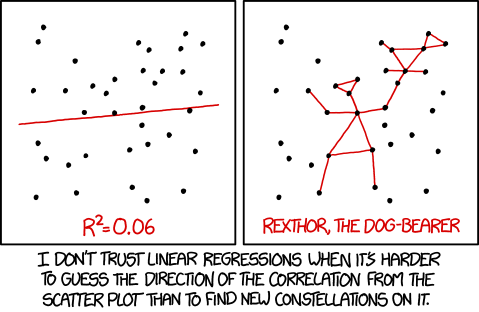
\includegraphics[width=12cm]{figures/linear_regression.png}}
\end{figure}


\subsection{ИП. Подготовка к битве}


\begin{enumerate}

\item Убедитесь, что в рамках классической модели $y=X\beta + u$ и предпосылок $\E(u) = 0$, $\Var(u) = \sigma^2 I$  умеете находить любые $\E()$, $\Var()$ и $\Cov(,)$ для векторов $\beta$, $\hb$, $y$, $\hy$, $u$, $\hat u$.

\item Вектор $u$ размера $4 \times 1$ имеет стандартное нормальное распределение, $u \sim \cN (0; I)$. Известен вектор $d$, $d=(1, -1, 2, -2)$.

\begin{enumerate}
  \item Найдите такую матрицу $H$, что её умноженение на произвольный вектор $y$ означает проецирование вектора $y$ на прямую порождённую вектором $d$
  \item Как распределена случайная величина $u' H u$? Чему равно её математическое ожидание и дисперсия?
\end{enumerate}

\item Вектор $u$ имеет стандартное нормальное распределение, $u \sim \cN (0; I)$. Матрица $A$ такова, что $Au$ также имеет стандартное нормальное распределение, $Au \sim \cN(0;I)$.
\begin{enumerate}
  \item Выпишите уравнение, которому подчиняется матрица $A$
  \item Чему может равняться $\det A$?
  \item Рассмотрим $c_1$ и $c_2$ — первый и второй столбец матрицы $A$. Найдите $c_1'c_1$ и $c_1'c_2$
\end{enumerate}

\item Предположим, что функция $f(x) = x'Ax + Bx + c$ имеет минимум. Найдите его, используя технику дифференциирования по вектору

\item Рассмотрим систему уравнений $X\beta = y$. Здесь $y$ — известный вектор размера $n\times 1$, $\beta$ — неизвестный вектор размера $k\times 1$, и $X$ — известная матрица размера $n\times k$ полного ранга. Мы хотим решить эту систему относительно $\beta$. Если $n=k$, то решать эту систему скучно, и, конечно, $\beta = X^{-1}y$. Гораздо интереснее решать систему, когда решений нет или когда их бесконечно много :)

\begin{enumerate}
\item Если решений нет, то найдите наилучшее приближение к решению, то есть такое $\beta$ при котором длина $(y-X\beta)$ минимальна.
\item Если решений, $\beta$, бесконечно много, то найдите решение с наименьшей длиной.
\end{enumerate}


\end{enumerate}

\begin{figure}[h!]
\floatbox[{\capbeside\thisfloatsetup{capbesideposition={right,bottom},capbesidewidth=4cm}}]{figure}[\FBwidth]
{\caption*{Randall Munroe, xkcd}}
{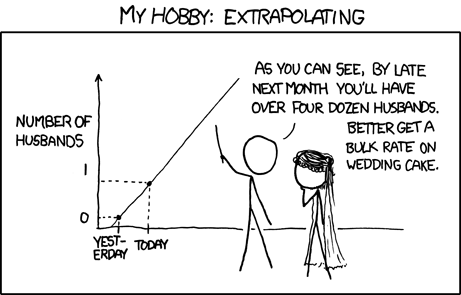
\includegraphics[width=10cm]{figures/extrapolating.png}}
\end{figure}

\subsection{ИП. Битва под Малоярославцем, 24.10.2016/24.10.1812}

\begin{enumerate}

\item Цель этой кампании — доказать теорему Гаусса-Маркова для множественной регрессии. Итак, $y=X\beta + u$, про случайные ошибки $u$ известно, что $\E(u)=0$, $\Var(u)=\sigma^2 \cdot I$. Поехали! :)

Тульский дворянин Дмитрий Сергеевич Дохтуров использует классическую МНК-оценку, $\hb_{OLS}$:

\begin{enumerate}
\item Вспомните формулу для МНК-оценки $\hat \beta_{OLS}$
\item Является ли оценка $\hat \beta_{OLS}$ линейной по $y$?
\item Докажите, что оценка $\hat \beta_{OLS}$ является несмещённой
\end{enumerate}

Корсиканец Наполеон Бонапарт предлагает альтернативную несмещённую оценку $\hb_{alt} = A\cdot y$:

\begin{enumerate}[resume]
\item Является ли оценка $\hb_{alt}$ линейной по $y$?
\item Чему равняется матрица $AX$? Да поможет здесь условие несмещённости!
\item Найдите $\Cov(\hb_{alt}, \hb_{OLS})$ и $\Cov(\hb_{OLS}, \hb_{alt})$.
\item Полученное в предыдущем пункте выражение должно вызывать ностальгию, так как очень похоже на\ldots~На что?
\end{enumerate}

Теперь пора посмотреть на разницу $\hb_{alt} - \hb_{OLS}$:

\begin{enumerate}[resume]
\item Вспомните или выведите формулу для $\Var(r + s)$, где $r$ и $s$ — случайные векторы одинакового размера
\item Докажите, что $\Var(\hb_{alt} - \hb_{OLS}) = \Var(\hb_{alt}) - \Var(\hb_{OLS})$
\item Рассмотрим матрицу $C = \Var(\hb_{alt}) - \Var(\hb_{OLS})$. Что находится на её диагонали?
\item Является ли матрица $C$ симметричной?
\item Докажите, что матрица $C$ является положительно полуопределённой. Если кто забыл, то это означает, что для любого вектора $a$ выполнено неравенство $a'Ca \geq 0$
\item Докажите, что диагональные элементы матрицы $C$ не меньше нуля
\end{enumerate}


\item Вектор $u$ размера $3 \times 1$ имеет стандартное нормальное распределение, $u \sim \cN (0; I)$. Дана матрица $D$:

\[
D = \frac{1}{14} \begin{pmatrix}
1 & 2 & 3 \\
2 & 4 & 6 \\
3 & 6 & 9
\end{pmatrix}
\]

\begin{enumerate}
  \item Является ли матрица $D$ симметричной? Идемпотентной?
  \item Найдите собственные числа матрицы $D$ с учётом кратности
  \item Как распределена случайная величина $u'Du$?
  \item Аккуратно объясните, в чём состоит геометрический смысл умножения произвольного вектора $y$ на матрицу $D$?
\end{enumerate}

\item Найдите величины $ESS$, $RSS$, $TSS$ и $R^2$ для регрессии $y_i = \mu + u_i$

\item В прошлом году, в курсе теории вероятностей и математической статистики, использовалось без доказательства следующее утверждение:

Если случайные величины $y_i$ независимы и нормально распределены $y_i \sim \cN (\mu; \sigma^2)$, то $q = \sum_{i=1}^n (y_i - \bar y)^2 / \sigma^2$ имеет хи-квадрат распределение с $(n - 1)$ степенью свободы.

Настала пора вернуть долг чести и доказать это утверждение :)

\begin{enumerate}
  \item Рассмотрим вектор центрированных $y$, то есть такой вектор $\tilde y$, что $\tilde y_i = y_i - \bar y$. Представьте вектор $\tilde y$ в виде $\tilde y = A y$. Как выглядит матрица $A$?
  \item Является ли матрица $A$ симметричной? Идемпотентной? Найдите все её собственные числа с учётом кратности.
  \item Представьте скаляр $q$ в виде $q= \frac{1}{\sigma^2} \tilde y' B \tilde y$. Как выглядит матрица $B$?
  \item Представьте скаляр $q$ в виде $q= \frac{1}{\sigma^2} y' C y$. Как выглядит матрица $C$?
  \item Представьте скаляр $q$ в виде $q= u' D u$, где вектор $u \sim \cN(0; I)$. Как выглядит матрица~$D$?
  \item Является ли матрица $D$ симметричной? Идемпотентной? Найдите все её собственные числа с учётом кратности.
  \item Сформулируйте теорему о законе распределение квадратичной формы нормальных случайных величин и верните долг чести.
\end{enumerate}


\end{enumerate}


\begin{figure}[h!]
% \floatbox[{\capbeside\thisfloatsetup{capbesideposition={right,bottom},capbesidewidth=4cm}}]{figure}[\FBwidth]
% {\caption*{Randall Munroe, xkcd}}
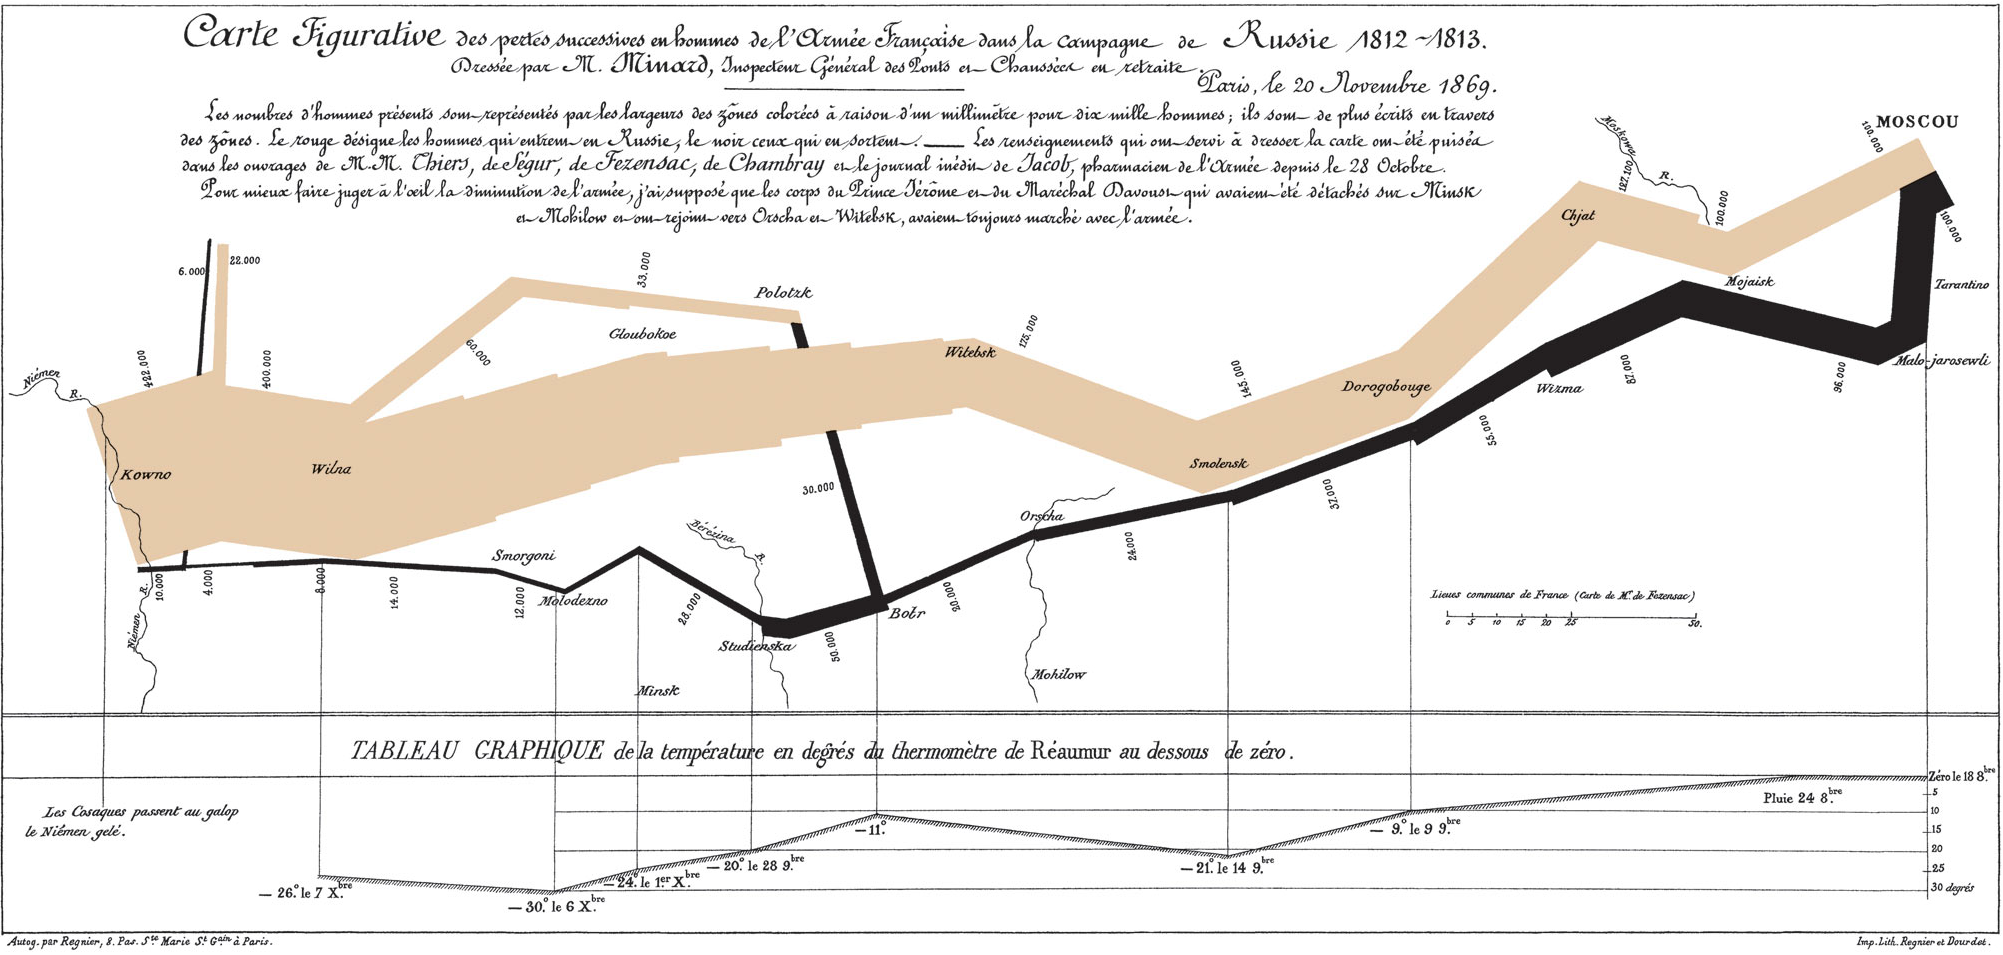
\includegraphics[width=19cm]{figures/Minard.png}
\caption*{Charles Joseph Minard, Схема потерь наполеоновской армии в компании 1812-1813 годов}
\end{figure}



\subsection{ИП. Битва — решения}

\begin{enumerate}

\item (25 points)
\begin{enumerate}
  \item (1)
  \item (1)
  \item (2)
  \item (2) Является, каждый элемент вектора оценок, это линейная комбинация значений $y$.
  \item (2)
\[
\E (\hb_{alt}) = \E (Ay) = A\E(y) = AX\beta = \beta \Rightarrow AX = I
\]
  \item (2)
\[
\Cov (Ay, (X'X)^{-1}X'y) = A  \Cov(y, y) X (X'X)^{-1} = \sigma^2 AX(X'X)^{-1} = \sigma^2 (X'X)^{-1}
\]
\[
\Cov ((X'X)^{-1}X'y, Ay) = (X'X)^{-1}X' \Cov(y, y) A' = \sigma^2 (X'X)^{-1} (AX)' = \sigma^2 (X'X)^{-1}
\]
  \item (2)
На ковариационную матрицу $\hb_{OLS}$!
  \item (2)
\[
\Var (r + s)
\]
Понятно, что на диагонали такой матрицы будут находится элементы следующего вида
\[
\Var(r_i + s_i) = \Var (r_i) + \Var (s_i) + 2\Cov (r_i, s_i)
\]
Все остальные элементы
\[
\Cov(r_i + s_i, r_j + s_j) = \Cov(r_i, r_j) + \Cov(r_i, s_j) +  \Cov(s_i, r_j) +  \Cov(s_i, s_j)
\]
Первое слагаемое принадлежит матрице $\Var (r)$, третье — $\Var(s)$, второе — $\Cov(r,s)$, четвертое — $\Cov(s,r)$. Получаем
\[
\Var(r + s) = \Var(r) + \Var (s) + \Cov(r,s) + \Cov(s,r)
\]
  \item (1)
\[
\Var (\hb_{alt} - \hb_{OLS}) = \Var(\hb_{alt}) + \Var(\hb_{OLS}) - 2\Cov (\hb_{alt}, \hb_{OLS}) =
\]
\[
\Var(\hb_{alt}) + \Var(\hb_{OLS}) - 2\Var(\hb_{OLS}) = \Var(\hb_{alt}) - \Var(\hb_{OLS})
\]
  \item (2)
На диагонали находится разница в дисперсиях коэффициентов.
  \item (2)
\[
\Var (Ay) = A \Var(y) A' = \sigma^2 AA'
\]
Поэтому $C$ симметрична,  как разница симметричных матриц.

  \item (4)
Константа не влияет на определенность матрицы, поэтому докажем этот факт без неё.
\[
a'Ca = a'(AA' - (X'X)^{-1})a = a'(AA' - AX(X'X)^{-1}X'A')a = a'A(I - H)A'a =
\]
\[
 a'A(I - H)(I - H)'A'a = ||(I - H)'A'a||^2_2 \geq 0
\]
  \item (2)
В матрице $C$ на диагонали находятся дисперсии разности оценок, а дисперсия всегда неотрицательна.
\end{enumerate}

\item (10)
\begin{enumerate}
  \item (2)
  Является симметричной и идемпотентной
  \item (3)
Можем посчитать по известной формуле, но лучше не надо :) Заметим, что ранг равен 1. Значит у нас 2 нулевых собственных значения. Матрица идемпотентна, значит третье собственное значение равно 1.
  \item (3)
Матрица $D$ представима в следующим виде:
\[
\frac{1}{14} (1, 2, 3)' (1,2,3) \Rightarrow u'Du = \frac{1}{14} u'(1, 2, 3)' (1,2,3)u
\]
$u'(1, 2,3)' $ — это сумма нормально распределенных случайных величин с некоторыми коэффициентами, такая сумма тоже имеет нормальное распределение c матожиданием 0 и дисперсией равной 14. Нормируя на корень из 14, мы получаем стандартную нормальную случайную величину. Значит
\[
\frac{1}{14} u'(1, 2, 3)' (1,2,3)u \sim \chi_1^2
\]

  \item (2)
Это проекция на пространство строк/столбцов матрицы $D$. В частности, на прямую, порожденную вектором (1,2,3).
\end{enumerate}

\item (7)

Оценка МНК даст $\mu = \overline{y}$.
\[
ESS = \sum (\hat{y}_i - \overline{y})^2 = \sum (\overline{y}- \overline{y})^2 = 0
\]
\[
RSS =  \sum (\hat{y}_i - y_i)^2 =  \sum (\overline{y} - y_i)^2  = TSS
\]
\[
R^2 = 0
\]

\item (16)
\begin{enumerate}
\item (2)
Пусть $G$ — матрица из одних единиц. Её смысл в том, что она будет суммировать элементы вектора, который был умножен на неё. Тогда
\[
A = I - \frac{1}{n}G
\]
\item (3)
\[
A' = A
\]
\[
(I - \frac{1}{n}G)(I - \frac{1}{n}G) = I -  \frac{1}{n}G - \frac{1}{n}G + \frac{1}{n^2}GG
\]
Легко видеть, что $GG$ — это матрица, где каждый элемент равен $n$. Получаем
\[
A^2 = A
\]

Заметим, что матрица $\frac{1}{n}G$ также идемпотентна. Значит её собственные значения равны единицам и нулям. Легко также видеть, что ранг равен 1. Значит у этой матрицы одно собственное значение равное 1, и все остальные равны 0. Умножая матрицу на $-1$, мы меняем знак собственных значений. А прибавляя единичную матрицу, мы увеличиваем все собственные значения на 1. Значит мы имеем $n-1$ единичное собственное значение, и одно собственное значение равное 0.

\item (1)
\[
B = I
\]
\item (3)
Чтобы перейти к равенству предыдущего пункта, нужно применить преобразование $A$ на вектора $y$. Тогда
\[
q = \frac{1}{\sigma^2}\tilde{y}' \tilde{y} =  \frac{1}{\sigma^2}y'A' A y \Rightarrow C = A' A
\]
\item (3)
Заметим, что деление $y$ на $\sigma$ нормирует вектор $y$.
\[
\frac{1}{\sigma^2}y'A' A y = \frac{1}{\sigma^2}y'A' A y = \left( \frac{\sigma u + \mu}{\sigma} \right)' A' A \left( \frac{\sigma u + \mu}{\sigma} \right) = (u + \frac{\mu}{\sigma})'A' A(u + \frac{\mu}{\sigma}) =
\]
Так как $A$ центрирует переменные, то $A\frac{\mu}{\sigma} = 0$, следовательно
\[
 (u + \mu)'A' A(u + \mu) = u'A'Au
\]
\[
D = A'A = AA = A
\]
\item (2)
Аналогично пункту б)
\item (3)
Осталось понять, какое распределение имеет $u'Au = u'(I - \frac{1}{n}G)u$. Как известно, матрицу $G$ можно представить в следующем виде
\[
\frac{1}{n}G = S\Lambda S'
\]
Где у матрицы лямбда все элементы 0 кроме элемента $S_{1,1}$. Пусть $s$ — это собственный вектор, который соответствует собственному значению $1$, тогда
\[
u'\frac{1}{n}Gu = u'ss'u
\]
Понятно, что собственный вектор с собственным значением $1$, это вектор констант, но так как в данном разложении матрица $S$ ортогональна, то длина собственного вектора $s$ равна 1. Тогда все элементы вектора $s$ равны $\frac{1}{\sqrt{n}}$.
\[
 u'ss'u = \left( \sum_{i = 1}^n \frac{u_i}{\sqrt{n}} \right)^2
\]
\[
\sum_{i = 1}^n \frac{u_i}{\sqrt{n}} \sim \mathbb{N} (0,1) \Rightarrow  u'ss'u \sim \chi_{1}^2
\]
\[
u'u \sim \chi_{n}^2 \Rightarrow q = u'Au \sim \chi_{n-1}^2
\]
\end{enumerate}
\end{enumerate}


\subsection{Кр 2, экзамен за I семестр, демо}

%<<child="tests/2016_kr_02_midterm_demo.Rnw">>=
%@

\AMCnumero{1} % сбрасываем номер вопроса на 1

\cleargroup{test}
%\copygroup[10]{midterm_demo_16}{test}
%\insertgroup{test}




\begin{enumerate}


\item На основании опроса была оценена следующая модель:
\[
\ln(wage_i)=\beta_1 + \beta_2 exper_i + \beta_3 age_i + \beta_4 sex_i + \e_i
\]

где:
\begin{itemize}
\item $wage_i$ — величина заработной платы в долларах
\item $exper_i$ — опыт работы в годах
\item $age_i$ — возраст в годах
\item $sex_i$ — пол (1 — мужской, 0 — женский)
\end{itemize}

\begin{tabular}{lr} \toprule
Показатель & Значение \\
\midrule
$R^2$                        & 0.903 \\
Скорректированный $R^2$      & \textbf{B7} \\
Стандартная ошибка регрессии & \textbf{B6} \\
Количество наблюдений        & \textbf{B2} \\
\bottomrule
\end{tabular}

Результаты дисперсионного анализа:

\begin{tabular}{lrrrrr} \toprule
 & df & SS & MS & F & P-значение \\
\midrule
Регрессия   &  3 & 2638.3  & 879.4 & \textbf{В5} & 0.000 \\
Остаток     & \textbf{B1} & 282.1 & 16.6 &    &       \\
Итого       & \textbf{B3}  & \textbf{B4}     &       &    &       \\
\bottomrule
\end{tabular}


\begin{tabular}{lrrrrrr} \toprule
Коэффициент & Оценка & $se(\hb)$ & t-статистика & P-Значение & Нижние 95\% & Верхние 95\% \\
\midrule
Константа & -6.96 & 12.38 & -0.56 & 0.58 & -33.08 & 19.16 \\
$exper$ & 2.65 & 0.32 & 8.38 & 0.000 & 1.98 & 3.32 \\
$age$ & \textbf{В8} & \textbf{В9} & 8.06 & 0.000 & 4.13 & 7.06 \\
$sex$ & -10.73 & 1.79 & \textbf{В10} & 0.000 & -14.49 & -6.95 \\
\bottomrule
\end{tabular}

\begin{enumerate}
\item Найдите пропущенные числа \textbf{B1}--\textbf{B10}.

\item Как изменятся результаты оценки регрессии, если переменную $sex_i$ переопределить так, чтобы 0 соответствовал мужчинам, 1 — женщинам?
\end{enumerate}

Ответ округляйте до 2-х знаков после запятой. Кратко поясняйте, например, формулой, как были получены результаты.



\item Юный эконометрист Вениамин очень любит опаздывать на первую пару. Он считает, что время (в минутах), на которое он опаздывает, $time_t$, зависит от количества снега (в миллиметрах), выпавшего за последние сутки, $snow_t$. После месяца упорного сбора данных, он смог оценить следующую модель:

\[
\widehat{time}_t=12+0.2snow_t
\]

Оценка ковариационной матрицы коэффициентов,
$\hVar(\hb) = \begin{pmatrix}
5 & -0.03 \\
-0.03 & 0.01\\
\end{pmatrix}$

Оценка дисперсии ошибок равна $\hs^2=1.45$.

За последние сутки выпало 15 миллиметров снега.

\begin{enumerate}
\item Постройте точечный прогноз времени опоздания Вениамина
\item Постройте 95\%-ый доверительный интервал для $\E(time_t |snow_t=15)$ для ожидаемого опоздания Вениамина
\item	Постройте 95\%-ый предиктивный интервал (доверительный интервал) для фактического опоздания Вениамина
\end{enumerate}


\item По данным 27 фирм, упорядоченных по капиталу, $K_1 < K_2 < \ldots < K_n$, была оценена зависимость выпуска $Y_i$ от труда $L_i$ и капитала $K_i$ с помощью моделей

\begin{enumerate}
\item[(1)] $\ln Y_i = \beta_1 + \beta_2 \ln L_i + \beta_3 \ln K_i + u_i$
\item[(2)] $\ln Y_i = \beta_1 + \beta_2 \ln \frac{L_i}{K_i} + u_i$
\end{enumerate}


\begin{tabular}{lD{.}{.}{3}cD{.}{.}{3}}
\toprule
&\multicolumn{1}{c}{Модель (1)}&&\multicolumn{1}{c}{Модель (2)}\\
\midrule
константа &1.1706&&1.0692\\
          &(0.326)&&(0.1317)\\
$\ln L$       &0.6029&&\\
          &(0.125)&&\\
$\ln K$       &0.375&&\\
          &(0.085)&&\\
$\ln \frac{L}{K}$    &&&0.6369\\
                     &&&(0.0754)\\
\midrule
R-squared&0.943 && 0.74 \\
F&200.24&&71.351\\
P-value&0.0&&0.0\\
RSS&0.851&&\\
N&27&&27\\
\bottomrule
\end{tabular}

\begin{enumerate}
\item На уровне значимости $\alpha = 0.05$ проверьте для модели (1) гипотезы $H_0$: $\beta_2 = \beta_3=0$ и $H_0$: $\beta_3=0.5$.
\item Объясните, почему модель (2) является ограниченной версией модели (1). Явно выпишите ограничения. На уровне значимости $\alpha = 0.05$ проверьте гипотезу об этих ограничениях.
\item Фирмы разделили на маленькие, $i \leq 14$, и большие, $i \geq 15$. Для этих двух групп оценили отдельные регрессии. Можно ли считать, что производственные функции для больших и маленьких фирм не различаются? Ответ подтвердите подходящим тестом.
\end{enumerate}

\begin{tabular}{lD{.}{.}{3}cD{.}{.}{3}}
\toprule
&\multicolumn{1}{c}{Модель для $i\leq 14$}&&\multicolumn{1}{c}{Модель для $i\geq 15$}\\
\midrule
константа &0.6998&&  1.4082\\
          &(0.649)&& (0.678)\\
$\ln L$   &0.9000&&  0.0081 \\
          &(0.133)&& (0.226)\\
$\ln K$   &0.2100&& 0.805\\
          &(0.056)&& (0.179)\\
\midrule
R-squared&0.896 && 0.908 \\
F&47.84&&49.81\\
P-value&0.0&&0.0\\
RSS&0.119&&0.362\\
N&14&&13\\
\bottomrule
\end{tabular}



\item С помощью теста Бокса-Кокса оценили зависимость веса индивида (в килограммах) от его роста (в сантиметрах):

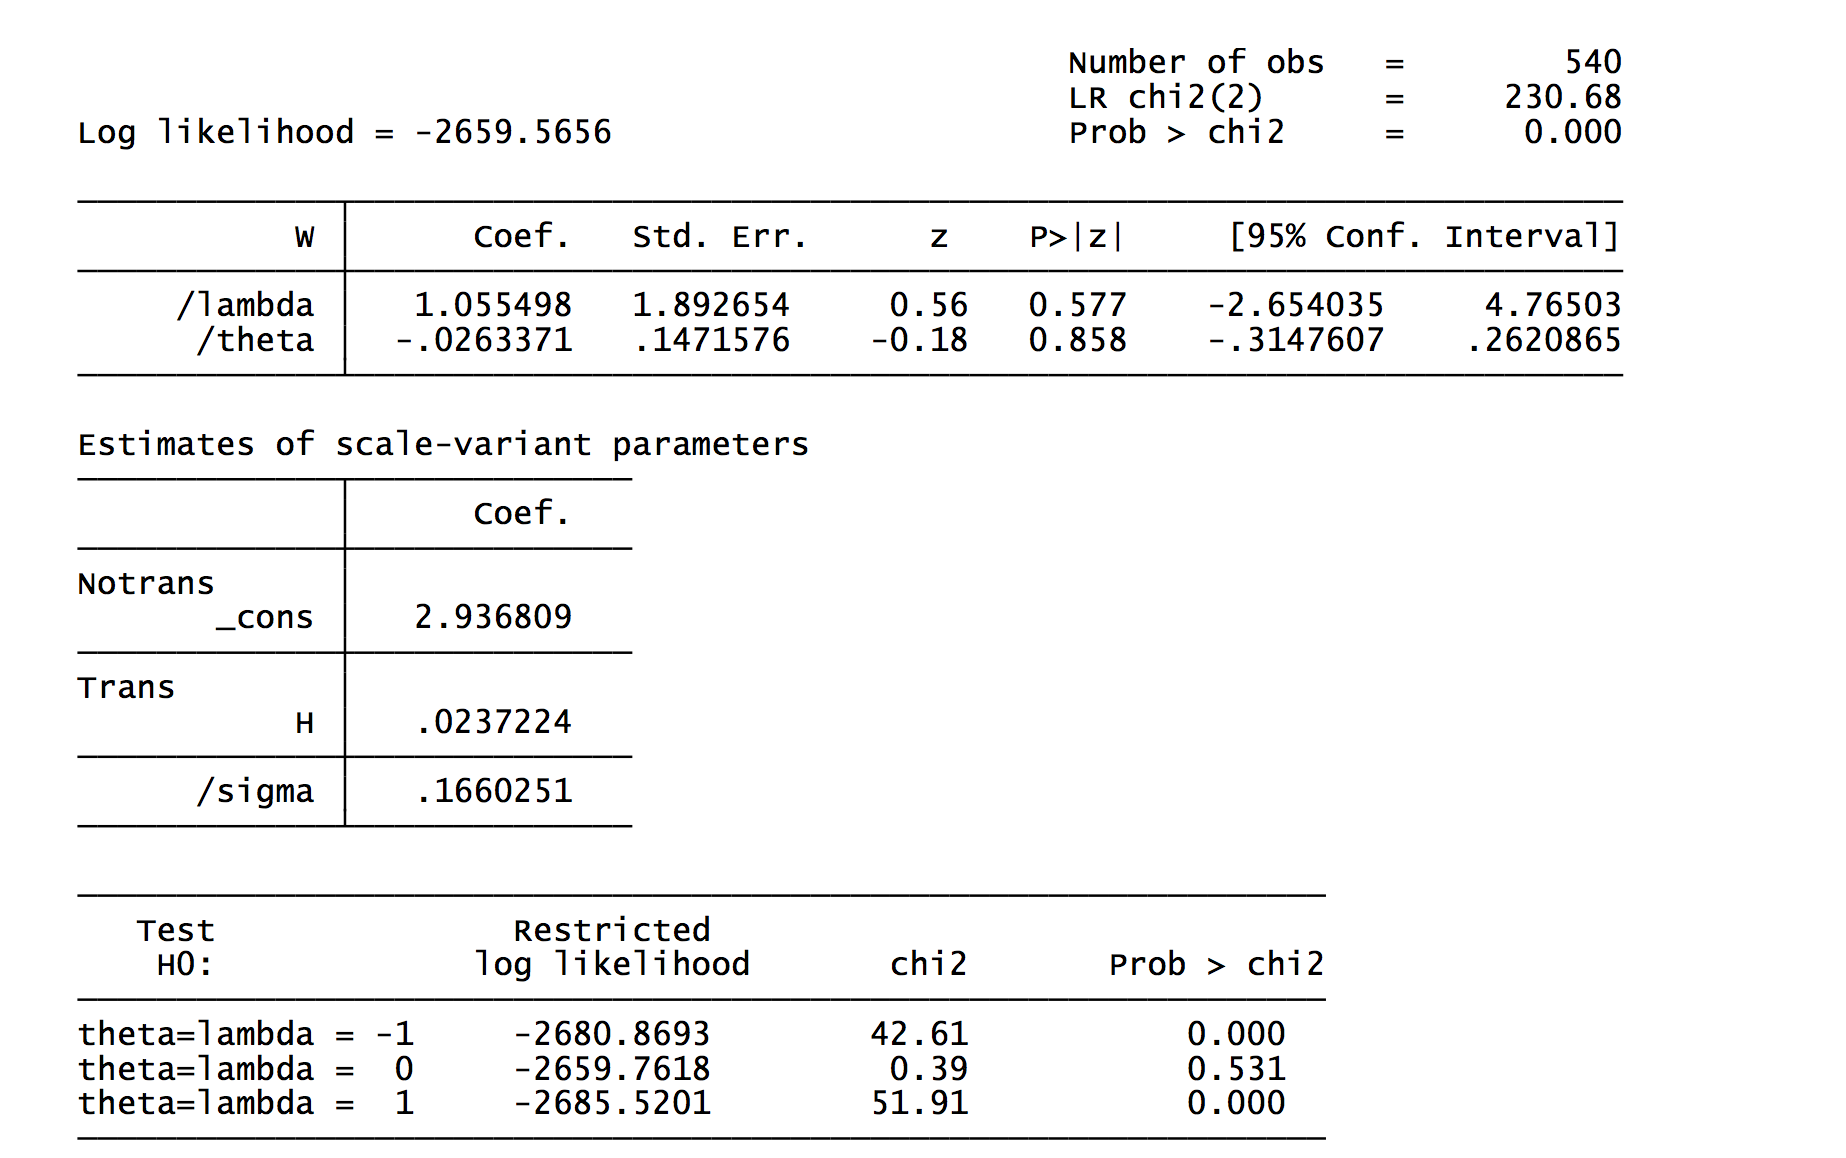
\includegraphics[width=\textwidth]{figures/box_cox.png}

Какую спецификацию модели (линейную, линейную в логарифмах, полулогарифмическую) следует предпочесть и почему?


\item По данным для  23 демократических стран оценили зависимость индекса Джини\footnote{Индекс Джини — это мера неравенства доходов. Чем выше индекс Джини, тем выше неравенство.} от ВВП на душу населения с учетом ППС (паритета покупательной способности). Затем провели тест Рамсея.

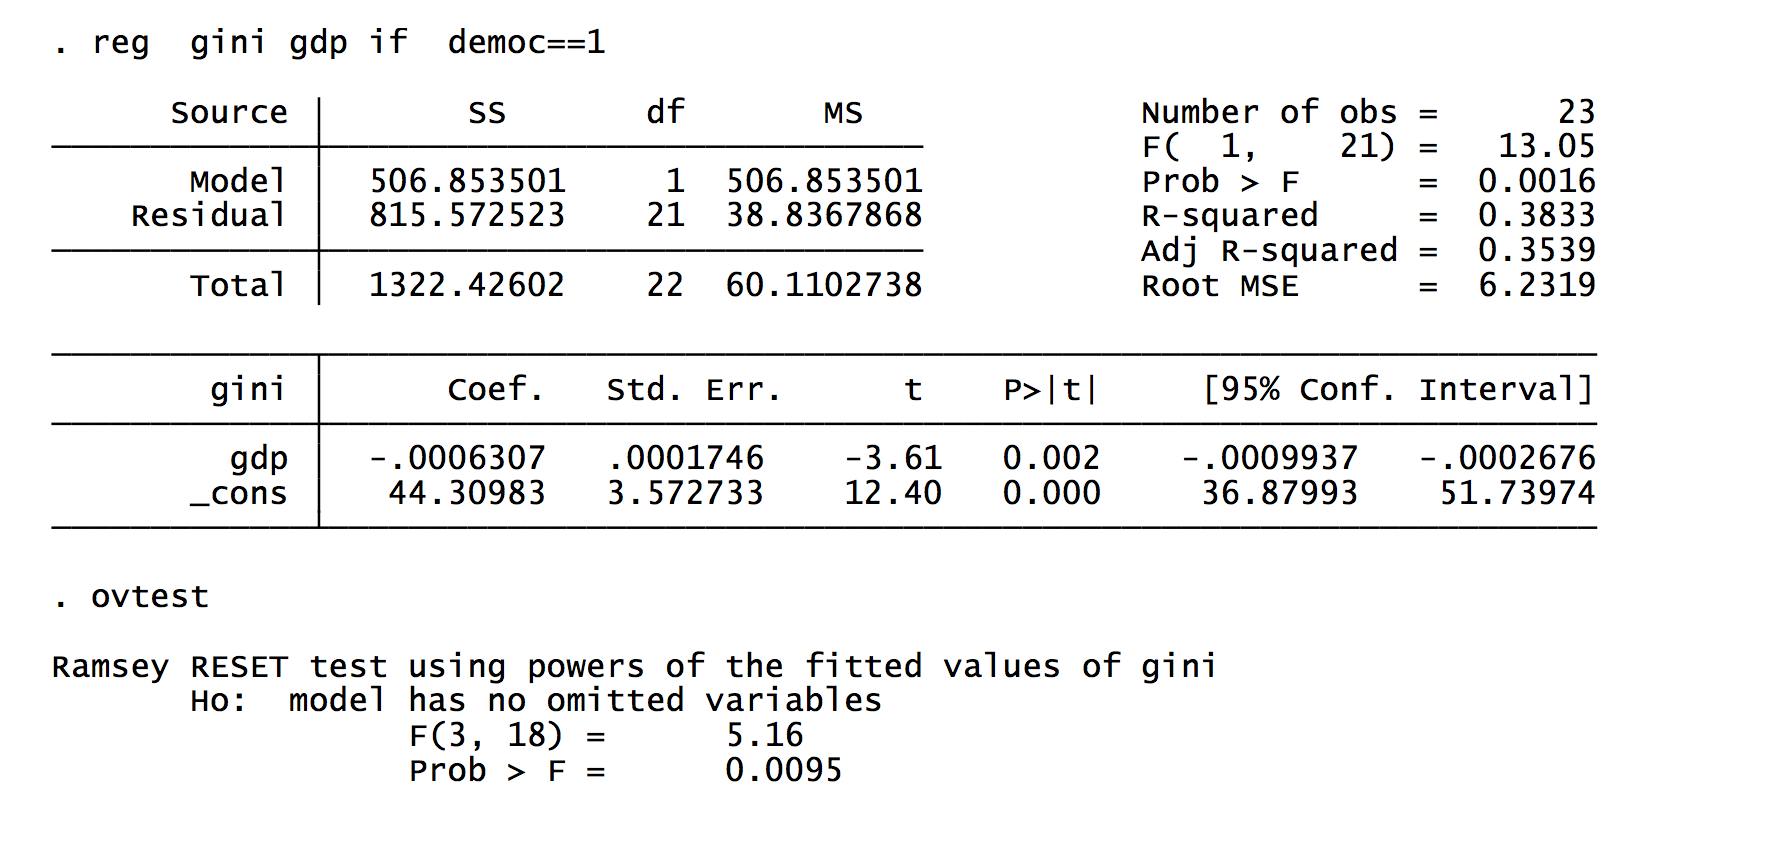
\includegraphics[width=\textwidth]{figures/ramsey.png}

\begin{enumerate}
\item Сформулируйте нулевую и альтернативную гипотезу теста Рамсея
\item Опишите пошагово, как проводится тест Рамсея
\item Прокомментируйте результаты теста Рамсея
\end{enumerate}

\end{enumerate}




\subsection{Кр 2, экзамен за I семестр, демо, решения}

\begin{enumerate}

\item
\begin{minted}[mathescape,
               linenos,
               numbersep=5pt,
               frame=lines,
               framesep=2mm]{r}
y_hat <- 12 + 0.2 * 15
se_y_hat <- 5 + 225 * 0.01 + 2 * 15 * 0.03
se_forecast_error <- se_y_hat + 1.45
t_crit <- qt(0.975, df = 30 - 2)
\end{minted}

\begin{enumerate}
\item
Или руками:

\textbf{B1}: Воспользуемся следующим соотношением:
\[
\frac{\text{Residual SS}}{\text{Residual df}} = \text{Residual MS} \Rightarrow \textbf{B1} = \text{Residual df} = 17
\]
\textbf{B2}: $\text{Residual df} = n - k \Rightarrow n = 21$

\textbf{B3}: $\text{Total df} = n - 1 = 20$

\textbf{B4}: $TSS = RSS + ESS \Rightarrow TSS = 2920.4$

\textbf{B5}: $F = \frac{\text{Regression MS}}{\text{Residual MS}} = \frac{879.4}{16.6} = 52.98$

\textbf{B6}: $\hat{\sigma}^2 = \frac{RSS}{n-k} = \frac{282.1}{21-4} = 16.59$

\textbf{B7}: $R^2_{adj} = 1 - \frac{RSS/(n-k)}{TSS/(n-1)} = 1 - \frac{282.1/17}{2920.4/20} = 0.87$

\textbf{B8} и \textbf{B9} получаются из следующей системы, где $2.11$ берётся из таблицы распределения Стьюдента, $t_{21-4;0.025}$:
\[
\begin{cases}
\hb_{age} - 2.11 \cdot se(\hb_{age}) = 4.13 \\
\hb_{age} + 2.11 \cdot se(\hb_{age}) = 7.06
\end{cases}
\Rightarrow
\begin{cases}
\hb_{age} = 5.63 \\
se(\hb_{age}) = 0.71
\end{cases}
\]
\textbf{B10}: $t_{obs} = \frac{\hb_{sex}}{se(\hb_{sex})} \Rightarrow t_{obs} = -5.99$
\item $\hb_{4, new} = -\hb_{4, old}$, $\hb_{1, new} = \hb_{1, old} - \hb_{4, new}$, остальные не изменятся.
\end{enumerate}
\item


\begin{minted}[mathescape,
               linenos,
               numbersep=5pt,
               frame=lines,
               framesep=2mm]{r}
t_obs <- (0.385 - 0.5) / 0.085
t_crit <- qt(0.975, df = 27 - 3)
F_obs <- (0.943 - 0.74) / (1 - 0.943) * (27 - 3)
F_crit <- qf(0.95, df1 = 1, df2 = 27 - 3)
\end{minted}

Или руками:
\begin{enumerate}
\item $\widehat{time}_f = 12 + 0.2 \cdot 15 = 15$
\item Доверительный интервал для среднего значения иммет вид:
\[
[\widehat{time}_f - z_{cr} \cdot se(\widehat{time}_f); \widehat{time}_f + z_{cr} \cdot se(\widehat{time}_f)]
\]
\begin{multline*}
\Var(\widehat{time}_f - \E(time_f | X)|X) = \Var(\widehat{time}_f|X) = \Var(\beta_1 + 15\beta_2 | X) = \\
= \Var(\beta_1|X) + 225 \Var(\beta_2|X) + 2 \cdot 15 \Cov(\beta_1, \beta_2|X) = 6.35 \\
\end{multline*}
\[
[15 - 2 \sqrt{6.35}; 15 + 2 \sqrt{6.35}]
\]
\item Доверительный (предиктивный) интервал для конкретного значения иммет вид:
\[
[\widehat{time}_f - z_{cr} \cdot se(\widehat{time}_f - \e_f); \widehat{time}_f+ z_{cr} \cdot se(\widehat{time}_f - \e_f)]
\]
\begin{multline*}
\Var(\widehat{time}_f - time_f | X) = \Var(\widehat{time}_f - \E(time_f | X) - \e_f |X) = \\
= \Var(\widehat{time}_f - \e_f |X) = \Var(\widehat{time}_f|X) + \Var(\e_f |X) = 6.35 + 1.45 = 7.8
\end{multline*}
\[
[15 - 2 \sqrt{7.8}; 15 + 2 \sqrt{7.8}]
\]
\end{enumerate}
\item
\begin{enumerate}
\item Гипотеза об адекватности множественной регрессии проверяется, с помощью следующей статистики:
\[
F = \frac{ESS/(k-1)}{RSS_{UR} / (n-k)} = \frac{R^2/(k-1)}{(1-R^2)/(n-k)}
\]
где $F \sim F_{k-1, n-k}$ при верной $H_0$. Найдём наблюдаеомое и критическое значения статистики:
\[
F_{obs} = \frac{0.943/2}{(1-0.943)/(27-3)} = 198.5 \quad \quad F_{crit} = 3.4
\]
Поскольку $F_{obs} > F_{crit}$, основная гипотеза отвергается.

Также можно было заметить, что в таблице уже дано $F = 200.24$ и сделать тот же вывод.

Проверим $H_0: \beta_3 = 0.5$:
\[
t_{obs} = \frac{\hb_3 - \beta_3}{se(\hb_3)} = \frac{0.375 - 0.5}{0.085} = -1.47 \quad \quad t_{crit} = 2.06
\]
Так как $|t_{obs}| < t_{crit}$, оснований отвергать $H_0$ нет.

\item Модель (2) получается из модели (1) при $\beta_3 = -\beta_2$. Будем проверять гипотезу $H_0: \beta_3 + \beta_2 = 0$.
\[
F_{obs} = \frac{RSS_{R} - RSS_{UR}/q}{RSS_{UR}/(n-k_{UR})} = \frac{(R^2_{UR} - R^2_{R})/q}{(1-R^2_{UR})/(n-k_{UR})} = \frac{(0.943-0.74)/1}{(1-0.943)/(27-3)}=85.47
\]
$F_{obs} > F_{crit} = 4.26 \Rightarrow$ основная гипотеза отвергается.
\item Введём дополнительную переменную:
\[
d_i = \begin{cases}
1, & i \leq 14 \\
0, & i > 14
\end{cases}
\]
Тогда можем записать неограниченную и ограниченную модели:
\[
UR: \ln Y_i = \beta_1 + \Delta_1 d_i + (\beta_2 + \Delta_2 d_i) \ln L_i + (\beta_3 + \Delta_3 d_i) \ln K_i + u_i
\]
\[
R: \ln Y_i =  \beta_1 + \beta_2  \ln L_i + \beta_3 \ln K_i + u_i
\]
Заметим, что $RSS_{UR} = 0.119 + 0.362 = 0.481$.

Будем проверять следующую гипотезу:
\[
H_0: \begin{cases}
\Delta_1 = 0 \\
\Delta_2 = 0 \\
\Delta_3 = 0
\end{cases}
\quad
H_a: \Delta_1^2 + \Delta_2^2 + \Delta_3^2 >0
\]
Для этого считаем F-статистику, $F \sim F_{3, 21}$ при верной $H_0$:
\[
F_{obs} = \frac{(RSS_R - RSS_{UR})/q}{RSS_{UR} / (n-k_{UR})} = \frac{(0.851-0.481)/3}{0.481/(27-6)} = 5.38 \quad \quad F_{crit} = 3.07
\]
Поскольку $F_{obs} > F_{crit}$, основная гипотеза отвергается.
\end{enumerate}

\item Гипотезы $H_0: \lambda = \theta = -1$ и $H_0: \lambda = \theta = 1$ (последняя соответсвует линейной спецификации) отвергаются.
Гипотеза $H_0: \lambda = \theta = 0$ (соответсвует логарифмической спецификации) не отвергается. Значит, преподпочтительной является логарифмическая модель.

\item
\begin{enumerate}
\item $H_0: gini_i = \beta_1 + \beta_2 \cdot gdp_i + u_i$, то есть в модели нет пропущенных переменных; $H_A:$ есть неизвсетные нам пропущенные регрессоры.
\item
\begin{itemize}
\item Оценить модель $gini_i = \beta_1 + \beta_2 \cdot gdp_i + u_i$, получить прогнозы $\widehat{gini}_i$.
\item Оценить вспомогательную регрессию $gini_i = \beta_1 + \beta_2 \cdot gdp_i + \gamma_1 \widehat{gini}_i^2 + \gamma_2 \widehat{gini}_i^3 + \ldots + \gamma_p \widehat{gini}_i^{p+1} + u_i$
\item Посчитать F-статистику, проверяющую гипотезу о равенстве всех $\gamma_i$ нулю. При верной $H_0$ и нормальности остатков $F \sim F_{p, n-k-p}$.
\end{itemize}
\item Основная гипотеза отвергается на любом разумном уровне значимости. Значит, в модели есть пропущенные факторы.
\end{enumerate}
\end{enumerate}



\subsection{Кр 2, экзамен за I семестр, 24.12.2016}

%<<child="tests/2016_kr_02_midterm.Rnw">>=
%@

\AMCnumero{1} % сбрасываем номер вопроса на 1

\cleargroup{test}
%\copygroup[10]{midterm_16}{test}
%\insertgroup{test}


\begin{enumerate}

\begin{minted}[mathescape,
               linenos,
               numbersep=5pt,
               frame=lines,
               framesep=2mm]{r}
set.seed(var_no)
n_obs <- 200
opros <- data_frame(exper = rnorm(n_obs, mean = 7, sd = 2),
                    exper2 = exper^2,
                    sex = sample(0:1, n_obs, rep = TRUE),
                    eps = rnorm(n_obs, sd = 2),
                    wage = 3 + 6 * exper - 0.2 * exper2 + 1.5 * sex + eps)
model <- lm(data = opros, wage ~ exper + exper2 + sex)
report <- summary(model)
coefs <- coef(model)
\end{minted}

\item На основании опроса 200 человек была оценена следующая модель:
\[
\ln(wage_i)=\beta_1 + \beta_2 exper_i + \beta_3 exper^2_i + \beta_4 sex_i + \e_i
\]

где:
\begin{itemize}
\item $wage_i$ — величина заработной платы в долларах
\item $exper_i$ — опыт работы в годах
\item $exper^2_i$ — опыт работы в годах
\item $sex_i$ — пол (1 — мужской, 0 — женский)
\end{itemize}

\begin{tabular}{lr} \toprule
Показатель & Значение \\
\midrule
$R^2$                        & 0.911 \\
Скорректированный $R^2$      & \textbf{B7} \\
Стандартная ошибка регрессии & \textbf{B6} \\
Количество наблюдений        & \textbf{B2} \\
\bottomrule
\end{tabular}

Результаты дисперсионного анализа:

\begin{tabular}{lrrrr} \toprule
            &  df           & сумма квадратов & F           & P-значение \\
\midrule
Регрессия   & 3            & \textbf{B9}     & \textbf{В5}  & 0.000 \\
Остаток     & \textbf{B1}  &  830.1          &              &       \\
Итого       & \textbf{B3}  & \textbf{B4}     &              &       \\
\bottomrule
\end{tabular}


\begin{table}[ht]
\centering
\begin{tabular}{rrrrr}
  \hline
 & Оценка & Ст. ошибка & t-статистика & P-Значение \\
  \hline
Константа & 3.6869 & 1.1960 & 3.08 & 0.0023 \\
  $exper$ & \textbf{В8} & 0.3525 & 16.45 & 0.0000 \\
  $exper^2$ & -0.1916 & 0.0254 & -7.54 & 0.0000 \\
  $sex$ & 1.5745 & 0.2937 & \textbf{В10} & 0.0000 \\
   \hline
\end{tabular}
\end{table}



\begin{enumerate}
\item Найдите пропущенные числа \textbf{B1}--\textbf{B10}.

\item Как изменятся результаты оценки регрессии, если переменную $sex_i$ переопределить так, чтобы 0 соответствовал мужчинам, 1 — женщинам?
\end{enumerate}

Ответ округляйте до 2-х знаков после запятой. Кратко поясняйте, например, формулой, как были получены результаты.

\item Исследовательница Глафира изучает зависимость спроса на молоко от цены молока и дохода семьи. В её распоряжении есть следующие переменные:

\begin{itemize}
\item $price$ — цена молока в рублях за литр
\item $income$ — ежемесячный доход семьи в тысячах рублей
\item $milk$ — расходы семьи на молоко за последние семь дней в рублях
\end{itemize}

В данных указано, проживает ли семья в сельской или городской местности. Поэтому Глафира оценила три регрессии: (All) — по всем данным, (Urban) — по городским семьям, (Rural) — по сельским семьям.

\begin{minted}[mathescape,
               linenos,
               numbersep=5pt,
               frame=lines,
               framesep=2mm]{r}
var_no <- 1
set.seed(var_no)
n_obs <- 100

milk_demand <- data_frame(
  eps = rnorm(n_obs, sd = 5),
  price = rnorm(n_obs, mean = 20, sd = 3),
  city = sample(0:1, n_obs, rep = TRUE),
  income = rnorm(n_obs, mean = 70, sd = 10))

milk_demand <- mutate(milk_demand, milk = ifelse(city == 1,
                                                 1 + 0.2 * income - 0.1 * price + eps,
                                                 0 + 0.3 * income - 0.5 * price + eps))

model_all <- lm(data = milk_demand, milk ~ income + price)
model_urban <- lm(data = filter(milk_demand, city == 1), milk ~ income + price)
model_rural <- lm(data = filter(milk_demand, city == 0), milk ~ income + price)

model_table <- mtable("(All)" = model_all, "(Urban)" = model_urban, "(Rural)" = model_rural,
                      summary.stats = c("R-squared", "adj. R-squared", "sigma", "F", "p", "Deviance", "N"))

model_table <- relabel(model_table, Deviance = "RSS", p = "P-value", N = "n observations")

toLatex(model_table)
\end{minted}



\begin{tabular}{lD{.}{.}{3}D{.}{.}{3}D{.}{.}{3}}
\toprule
 &
\multicolumn{1}{c}{(All)} &
\multicolumn{1}{c}{(Urban)} &
\multicolumn{1}{c}{(Rural)}\\
\midrule
(Intercept)    &  1.479       & -0.797     &  4.598      \\
               & (4.480)      & (7.808)    & (5.121)     \\
income         &  0.252^{***} &  0.204^{*} &  0.262^{***}\\
               & (0.049)      & (0.092)    & (0.053)     \\
price          & -0.335^{*}   &  0.001     & -0.567^{**} \\
               & (0.165)      & (0.272)    & (0.194)     \\
\midrule
R-squared      &    0.230 &    0.104 &   0.380\\
adj. R-squared &    0.214 &    0.063 &   0.355\\
sigma          &    4.678 &    5.036 &   4.160\\
F              &   14.464 &    2.541 &  15.326\\
P-value        &    0.000 &    0.090 &   0.000\\
RSS            & 2123.000 & 1115.693 & 865.080\\
n observations &  100     &   47     &  53    \\
\bottomrule
\end{tabular}



\begin{enumerate}
\item Проверьте значимость в целом регрессии (All) на 5\%-ом уровне значимости.
\item На 5\%-ом уровне значимости проверьте гипотезу, что зависимость спроса на молоко является единой для городской и сельской местности.
\end{enumerate}

\item Исследовательница Глафира продолжает изучать спрос на молоко. В её распоряжении по-прежнему данные по трём переменным:
\begin{itemize}
\item $price$ — цена молока в рублях за литр
\item $income$ — ежемесячный доход семьи в тысячах рублей
\item $milk$ — расходы семьи на молоко за последние семь дней в рублях
\end{itemize}

Имеются результаты оценивания модели $milk_i = \beta_1 + \beta_2 income_i + \beta_3 price_i + u_i$ по $100$ наблюдениям:
\begin{minted}[mathescape,
               linenos,
               numbersep=5pt,
               frame=lines,
               framesep=2mm]{r}
xtable(model_all)
\end{minted}


\begin{tabular}{rrrrr}
  \hline
 & Estimate & Std. Error & t value & Pr($>$$|$t$|$) \\
  \hline
(Intercept) & 1.4791 & 4.4796 & 0.33 & 0.7420 \\
  income & 0.2524 & 0.0486 & 5.19 & 0.0000 \\
  price & -0.3354 & 0.1649 & -2.03 & 0.0447 \\
   \hline
\end{tabular}



Коэффициент детерминации $R^2$ оказался равен $0.23$.


Глафира рассчитала оценку ковариационной матрицы исходных переменных:

\begin{minted}[mathescape,
               linenos,
               numbersep=5pt,
               frame=lines,
               framesep=2mm]{r}
xtable(var(dplyr::select(milk_demand, price, income, milk)))
\end{minted}


\begin{tabular}{rrrr}
  \hline
 & price & income & milk \\
  \hline
price & 8.26 & 3.48 & -1.89 \\
  income & 3.48 & 95.09 & 22.83 \\
  milk & -1.89 & 22.83 & 27.84 \\
   \hline
\end{tabular}



\begin{enumerate}
\item Постройте точечный прогноз расходов на молоко семьи c доходом 100 тысяч рублей при цене на молоко 30 рублей за литр.
\item Найдите выборочную корреляцию между фактическими расходами на молоко и их прогнозами.
\item Разложите коэффициент детерминации $R^2$ в модели в сумму эффектов переменных $income$ и $price$.
\end{enumerate}


\item По квартальным данным 1958-1976 годов была оценена модель с тремя объясняющими факторами:
\[
\hat Y_i = 2.2 + 0.104 X_i - 3.48 Z_i + 0.34 W_i, \; ESS = 100, \; RSS = 120
\]

\begin{enumerate}
\item Какую модель необходимо оценить исследователю, если он считает, что в различные сезоны среднее значение зависимой переменной помимо зависимости от трёх регрессоров может отличаться на константу?
\item При оценивании модели, допускающей сезонные эффекты, оказалось, что значение $ESS$ увеличилось до $160$.
На уровне значимости 5\% проверьте гипотезу о наличии сезонности.
\end{enumerate}

\begin{minted}[mathescape,
               linenos,
               numbersep=5pt,
               frame=lines,
               framesep=2mm]{r}
set.seed(var_no)
hb_w <- sample(c(3, 4, 5), 1)
hb_r <- sample(c(6, 7, 8), 1)

X <- mvtnorm::rmvnorm(n = 24, mean = c(1, 1, 1),
             sigma = matrix(c(0, 0, 0, 0, 0.4, -0.1, 0, -0.1, 0.9), nrow = 3))
XXm <- solve(crossprod(X))
xmatrix <- function(a, environment = "pmatrix", output = TRUE, digits = 3) {

  # override default alignment for xtable
  xa <- xtable::xtable(a, align = rep("", ncol(a) + 1), digits = digits)

  res <- print(xa,
               floating = FALSE,
               tabular.environment = environment,
               hline.after = NULL,
               include.rownames = FALSE,
               include.colnames = FALSE,
               file = "junk.txt")

  res <- paste0("\\ensuremath{", res, "}")

  if (output) {
    cat(res)
  }
  return(invisible(res))
}
xmatrix(XXm)
\end{minted}

\item По 24 наблюдениям была оценена модель:

\[
\widehat{Y}_i=15-4Z_i+3W_i
\]

Известно, что случайные ошибки нормально распределены, $RSS=180$, и

\[
(X'X)^{-1} =
\begin{pmatrix}
  0.365 & -0.218 & -0.084 \\
  -0.218 & 0.184 & 0.027 \\
  -0.084 & 0.027 & 0.046 \\
  \end{pmatrix}
\]


\begin{enumerate}
\item Проверьте гипотезу $H_0: \beta_Z = 0$ против $H_a: \beta_Z \neq 0$ на уровне значимости~5\%.
\item Проверьте гипотезу $H_0: \beta_Z + \beta_W = 0$  против $H_a: \beta_Z + \beta_W \neq 0$ на уровне значимости~5\%.
\item Выпишите использованные при проверке гипотез предпосылки о случайных ошибках модели.
\end{enumerate}


\end{enumerate}

\subsection{Кр 2, экзамен за I семестр, 24.12.2016, решения}

\begin{enumerate}
\item
\begin{enumerate}
  \item
$\textbf{B1} = n - k = 200 - 4 = 196$

Из условия, $\textbf{B2} = n = 200$

$\textbf{B3} = n - 1  = 199$

Для нахождения \textbf{B4} воспользуемся знанием значения $R^2$:
\[
R^2 = 1 - \frac{RSS}{TSS} = 1 - \frac{830.1}{\textbf{B4}} = 0.911 \Rightarrow \textbf{B4} = 9326.97
\]
Для того, чтобы найти \textbf{B5}, понадобится $\textbf{B9} = TSS - RSS = 8496.87$. Тогда:
\[
\textbf{B5} = F = \frac{\text{Regression MS}}{\text{Residual MS}} = \frac{8496.87/3}{830.1/196} = 668.75
\]
\[
\textbf{B6} = \hat{\sigma}^2 = \frac{RSS}{n-k} = 4.24
\]
\[
\textbf{B7} = R^2_{adj} = 1 - \frac{RSS/(n-k)}{TSS/(n-1)} = 0.91
\]
Значение \textbf{B8} находится из соотношения:
\[
\frac{\hb}{se(\hb)} = t_{obs} \Rightarrow \textbf{B8} = 5.8
\]
Аналогично, для \textbf{B10}, $\textbf{B10} = 5.36$.

\item  $\hb_{4, new} = -\hb_{4, old}$, $\hb_{1, new} = \hb_{1, old} - \hb_{4, new}$, остальные не изменятся.
\end{enumerate}
\item
\begin{enumerate}
\item Необходимо проверить следующую гипотезу:
\[
H_0: \begin{cases}
\beta_1 = 0 \\
\beta_2 = 0 \\
\beta_3 = 0
\end{cases}
\quad
H_a: \beta_1^2 + \beta_2^2 + \beta_3^2 >0
\]
Для этого вопользуемся F-статистикой, $F \sim F_{2,97}$, она дана в таблице:
\[
F_{obs} = \frac{ESS/(k-1)}{RSS_{UR}/(n-k_{UR})} = 14.464
\]
Находим $F_{crit} = 3.09$. Поскольку $F_{obs} > F_{crit}$, гипотеза отвергается.

\item Для того, чтобы записать спецификацию неограниченной модели, введём дополнительную переменную $d_i$:
\[
d_i = \begin{cases}
1 & \text{городская местность} \\
0 & \text{сельская местоность}
\end{cases}
\]
Пусть коэффициенты для городской местности отличаются на некоторое $\Delta_i$, тогда неограниченная модель имеет вид:
\[
milk_i = \beta_1 + \Delta_1 d_i + (\beta_2 + \Delta_2 d_i) price_i + (\beta_3 + \Delta_3 d_i) income_i + \e_i
\]
\[
RSS_{UR} = RSS_{Urban} + RSS_{Rural} = 1115.693 + 865.08 = 1980.773
\]
Проверяем следующую гипотезу:
\[
H_0: \begin{cases}
\Delta_1 = 0 \\
\Delta_2 = 0 \\
\Delta_3 = 0
\end{cases}
\quad
H_a: \Delta_1^2 + \Delta_2^2 + \Delta_3^2 >0
\]
Для этого считаем F-статистику, $F \sim F_{3, 94}$ при верной $H_0$:
\[
F_{obs} = \frac{(2123 - 1980.773)/3}{1980.773/94} \approx 2.25
\]
Сравниваем с $F_{crit} = 2.7$, $F_{obs} < F_{crit} \Rightarrow$ нет оснований отвергать гипотезу.
\end{enumerate}
\item
\begin{enumerate}
\item $\widehat{milk} = 1.4791 + 0.2524 \cdot 100 - 0.3354 \cdot 30 = 16.6571$
\item $\sCorr(milk, \widehat{milk}) = \sqrt{R^2} = \sqrt{0.23}$
\item $R^2 = \sum_{j=2}^{k} \hb_j \frac{\sCov(x_j, y)}{\sVar(y)} = 0.2524 \cdot \frac{22.83}{27.84} - 0.3354 \cdot \frac{(-1.89)}{27.84}$
\end{enumerate}
\item
\begin{enumerate}
\item В модель необходимо добавить фиктивные переменные $Q_1$, $Q_2$ и $Q_3$, соответствующие первым трём кварталам года:
\[
Y_i = \beta_1 + \beta_2 X_i + \beta_3 Z_i + \beta_4 W_i + \beta_5 Q_{1i} + \beta_6 Q_{2i} + \beta_7 Q_{3i} + \e_i
\]
\item Гипотеза о наличии (а на самом деле отсутствии) сезонности записывается следущим образом:
\[
H_0: \begin{cases}
\beta_5 = 0 \\
\beta_6 = 0 \\
\beta_7 = 0
\end{cases}
\quad
H_{a}: \beta_5^2 + \beta_6^2 + \beta_7^2 > 0
\]
Поскольку гипотезы оцениваются по одним и тем же данным, $TSS$ в них совпадает и равен $ESS_{R} + RSS_{R} = 100 + 120 = 220$

Тогда в неограниченной модели $RSS_{UR} = 220 - 160 = 60$.

Количество наблюдений: $(1976-1958+1)\cdot 4 = 76$. Считаем, что данные взяты с первого квартала 1958 года по четвёртый квартал 1976 года.

Теперь можно проверять гипотезу, $F \sim F(3, 69)$:
\[
F_{obs} = \frac{(RSS_{R} - RSS_{UR}) / q}{RSS_{UR}/(n-k_{UR})} = \frac{(120 - 60) / 3}{40/69} = 34.5
\]
Так как $F_{obs} > F_{crit} = 2.73$, гипотеза отвергается.
\end{enumerate}

\item
\begin{enumerate}
\item Чтобы найти $se(\beta_Z)$, сначала найдём стандартную ошибку регрессии $\sigma^2$:
\[
\sigma^2 = \frac{RSS}{n-k} = \frac{180}{24-3} \approx 8.57
\]
Тогда $se(\beta_Z) = \sqrt{8.57 \cdot 0.184} = \sqrt{1.57688}$. Теперь можно проверять гипотезу:
\[
t_{obs} = \frac{-4}{\sqrt{1.57688}} \approx -3.19 \quad t_{crit} = -2.08
\]
Основная гипотеза отвергается.
\item t-статистика имеет вид:
\[
t_{obs} = \frac{\hb_Z + \hb_W - 0}{se(\hb_Z + \hb_W)} = \frac{-4 + 3}{\sqrt{8.57(0.184 + 0.046 + 2 \cdot 0.027)}} \approx -0.64 \quad t_{crit} \approx 2.08
\]
Нет оснований отвергать $H_0$.
\item $u_i \sim \cN(0, \sigma_u^2)$
\end{enumerate}
\end{enumerate}


\subsection{Кр 3, задачи для подготовки}

\url{https://www.hse.ru/mirror/pubs/share/203792575}

\subsection{Кр 3, 20.03.2017}


\subsubsection*{Часть 1. Тест.}

%<<child="tests/2016_kr_03.Rnw">>=
%@


\AMCnumero{1} % сбрасываем номер вопроса на 1

\cleargroup{test}
%\copygroup[10]{kr_03}{test}
%\insertgroup{test}


\subsubsection*{Часть 2. Задачи.}


\begin{enumerate}

\item По данным для 39 районов Балтимора в 1970 г. были оценены уравнения
\[\ln {\hat Y_i} = \mathop {10.093}\limits_{t = 54.7}  - \mathop {0.239}\limits_{t =  - 12.28} {X_i},\quad {R^2} = 0.803\]
и
\[\frac{{\ln {{\hat Y}_i}}}{{\sqrt {{X_i}} }} = \mathop {9.093}\limits_{t = 47.87} \frac{1}{{\sqrt {{X_i}} }} - \mathop {0.2258}\limits_{t =  - 15.10} \sqrt {{X_i}} ,\]
где $Y_i$ — плотность населения района, $X_i$ — расстояние до центрального делового квартала.

\begin{enumerate}
\item С какой целью оценили второе уравнение? Какое при этом было сделано предположение о дисперсии ошибок?
\item Дайте интерпретацию полученным результатам.
\end{enumerate}

\item Были обследованы 36 предприятий по трём показателям:  $K_i$ — основным фондам (млн. руб.), $W_i$ — фонду оплаты труда (млн. руб.), $R_i$ — расходам на НИОКР (млн. руб.). Получены оценки вектора средних $\hat \mu = (3, 4, 1)'$ и ковариационной матрицы  $\hat\Sigma = \begin{pmatrix}
2 & 3 & 0 \\
3 & 10 & 0 \\
0 & 0 & 3 \\
\end{pmatrix}
$.

Найдите первую главную компоненту и определите долю суммарной дисперсии, которую она объясняет.

\item Мартовский Заяц и Безумный Шляпник почти все время пьют чай. Известно, что количество выпитого за день чая (в чашках) зависит от количества пирожных (в штуках) и печенья (в штуках). Алиса, гостившая у героев в течение 25 дней, заметила, что если оценить зависимость выпитого чая от закуски для Мартовского Зайца и Шляпника
\[
Tea_i = \beta_1 + \beta_2 Biscuit_i + \beta_3 Cake_i + u_i,
\]
то получится регрессия с $RSS = 17$.

Чтобы понять, удачную ли модель она построила, Алиса оценила еще одну регрессию
\[
Tea_i = \beta_1 + \beta_2 Biscuit_i + \beta_3 Cake_i +
   +\gamma_2 \widehat{Tea_i^2} +\gamma_3 \widehat{Tea_i^3} +\gamma_4 \widehat{Tea_i^4} + \nu_i,
\]
с $RSS = 10$.

Помогите Алисе понять, верную ли спецификацию модели она выбрала: сформулируйте основную и альтернативную гипотезы и проведите подходящий тест.



\end{enumerate}

\subsection{Кр 3, 20.03.2017, решения}
\begin{enumerate}
  \item Второе уравнение оценили для корректного построения доверительных интервалов и проверки гипотез о коэффициентах в условиях гетероскедастичности, для получения более эффективных оценок, $\Var(u_i)=\sigma^2 X_i$.

  После применения взвешенного МНК оба коэффициента значимы.
  \item

Собственные значения ковариационной матрицы: $\lambda_1 = 11$, $\lambda_2 = 3$, $\lambda_3 = 1$.

Первая главная компонента: $(1/\sqrt{10} \quad 3/\sqrt{10} \quad 0)'$.

Доля дисперсии: $\frac{11}{15}$

  \item
  \[
  F = \frac{(RSS_R - RSS_{UR})/3}{RSS_{UR}/(n-k_{UR})}= \frac{(17-10)/3}{10/(25-6)} = 4.4(3)
  \]

\end{enumerate}



\subsection{ИП. Комоедица, 24.03.2016}


Комоедица — белорусский народный праздник, посвящённый пробуждению медведя :)


\begin{enumerate}

\item Докажем свойства оценок максимального правдоподобия!


Пусть $L(y|\theta)$ — функция правдоподобия, $y$ — вектор-столбец из $n$ наблюдений, $\theta$ — вектор-столбец из $m$ параметров. Кроме того, введём дополнительные обозначения, $\ell(\theta)=\ln L(y|\theta)$, $s(\theta) = \partial \ell/\partial \theta$. Буква $s$ сокращает слово «score».

Для наших целей мы определим информацию Фишера как $I=\Var(s(\theta))$. То есть информация Фишера — это ковариационная матрица первых производных лог-функции правдоподобия. По определению.


\begin{enumerate}
  \item Чтобы взбодриться, укажите размеры векторов и матриц $s(\theta)$, $\E(s(\theta))$, $\Var(s(\theta))$.
  \item Собрав всю силу воли в кулак, найдите $\E(1)$.
  \item Запишите $\E(1)$ с помощью интеграла по $dy$ и функции правдоподобия $L()$.
  \item Продифференциировав обе части найденного тождества по $\theta_j$, найдите $\int \frac{\partial L}{\partial \theta_j} \, dy$.
  \item Найдите $\E\left( \frac{\partial \ell}{\partial \theta_j} \right)$.
  \item Найдите $\E(s(\theta))$.
  \item Докажите, что $I=\E(s(\theta)s(\theta)')$.
  \item Вспомнив магию дифференциирования ещё раз, найдите    $\int \frac{\partial^2 L}{\partial \theta_j\partial \theta_i} \, dy$.
  \item Найдите $\E\left(\frac{\partial^2 L}{\partial \theta_j\partial \theta_i} \frac{1}{L}\right)$.
  \item Выразите $\frac{\partial^2 \ell}{\partial \theta_j\partial \theta_i}$ через $\frac{\partial \ell}{\partial \theta_j}$, $\frac{\partial \ell}{\partial \theta_i}$ и $\frac{\partial^2 L}{\partial \theta_j\partial \theta_i}$.
  \item Докажите, что $\E(\frac{\partial^2 \ell}{\partial \theta_j\partial \theta_i}) = - \E\left(\frac{\partial \ell}{\partial \theta_j} \frac{\partial \ell}{\partial \theta_i}\right)$.
  \item Докажите, что $I=-\E\left(\frac{\partial^2 \ell}{\partial \theta\partial \theta'}\right)$.

\end{enumerate}

\item ML в линейных моделях:

Можно смело считать первое упражнение сделанным, то есть использовать тот факт, что $I=-E(\frac{\partial^2 \ell}{\partial \theta\partial\theta'})$.

Рассмотрим задачу линейной регрессии, $y=X\beta+u$, где $u\sim \cN(0;\sigma^2)$. Для удобства определим $x_i'$ — $i$-ую строку матрицы $X$ и будем считать регрессоры неслучайными.

В нашем случае $\theta=(\beta', \sigma^2)'$.


Хинты для забывших матричное дифференцирование: $\frac{\partial Ar}{\partial r}=A$, $\frac{\partial^2 r'Ar}{\partial r\partial r'}=A+A'$, $\frac{\partial r'Ar}{\partial r'}=Ar+A'r$.

\begin{enumerate}
\item Выпишите $\ell(\theta)$ в виде суммы.
\item Выпишите вектор $s(\theta)$ в виде
$s(\theta) = \begin{pmatrix}
? \\
? \\
\end{pmatrix}$, где первый элемент — это сразу вектор производных по всем $\beta$ одним махом.
\item Найдите ML оценки $\hat\theta$.
\item Докажите, что $L(\hat\theta)=a \cdot RSS^{b}$, где $a$ и $b$ — некоторые константы. Забейте на $a$ и найдите $b$.
\item Найдите $\frac{\partial^2 \ell}{\partial \theta\partial\theta'}$ в виде четырёх блоков:
\[
\frac{\partial^2 \ell}{\partial \theta\partial\theta'}=\begin{pmatrix}
\frac{\partial^2 \ell}{\partial \beta\partial\beta'} & \frac{\partial^2 \ell}{\partial \beta\partial \sigma^2} \\
\frac{\partial^2 \ell}{\partial \sigma^2\partial\beta'} & \frac{\partial^2 \ell}{\partial \sigma^2\partial\sigma^2} \\
\end{pmatrix}.
\]
\item В предыдущем пункте все блоки должны были получится ненулевые. Однако найдите $I$ и пара блоков занулится :)
\item Найдите $I^{-1}$.
\end{enumerate}

\item Выведите формулу для $R^2$ в регрессии вектора $y=X\beta+u$.

\item LM-тест в линейных моделях.

Обозначим: $\hat\theta_R$ и $\hat\theta_{UR}$ — ограниченные и неограниченные экстремумы правдоподобия, а $\hat u_R$ и $\hat u_{UR}$ — соответствующие остатки.

Определим LM статистику как $LM = s(\hat\theta_R)'\widehat{\Var}^{-1}(s)s(\hat\theta_R)$.

Будем считать первое упражнение сделанным, поэтому
\[
LM = s(\hat\theta_R)'I^{-1}(\hat\theta_R)s(\hat\theta_R).
\]

Также можно считать сделанным второе упражнение, поэтому:
\[
s=\begin{pmatrix}
\frac{X'u}{\sigma^2} \\
\frac{u'u - n\sigma^2}{2\sigma^4} \\
\end{pmatrix}, \quad
I^{-1} =
\begin{pmatrix}
\sigma^2(X'X)^{-1} & 0 \\
0 & \frac{2\sigma^4}{n} \\
\end{pmatrix}.
\]

\begin{enumerate}
\item Кстати, а чему равно $s(\hat\theta_{UR})$?
\item Найдите $s(\hat\theta_R)$ и $I^{-1}(\hat\theta_R)$.
\item Выведите формулу для $LM$ статистики, содержащую только $X$, $\hat u_R$ и $n$.
\item Какую регрессию надо построить, чтобы $R^2$ в ней оказался таким, что $LM=nR^2$?
\end{enumerate}


\item Исследовательница Елизавета оценила модель множественной регрессии, $y=X\beta + u$. Затем Елизавета проверяет гипотезу о незначимости отдельного коэффициента $\beta_j$ двумя способами: через $t$-статистику и через $F$-статистику с ограниченной и неограниченной регрессией.

Докажите, что $t^2 = F$.


\item Василий обнаружил странную монетку и решил произвести над ней эксперименты. Выпадение орла он кодирует $y_i=1$, решки — $y_i=0$.

При известном параметре $p$, наблюдаемые $y_1$, \ldots, $y_n$ независимы и имеют распределение Бернулли, $y_i|p \sim Bernoulli(p)$. Априорно по мнению Василия параметр $p$ имеет бета-распределение, $p \sim beta(\alpha, \beta)$, где $\alpha$ и $\beta$ — некоторые неслучайные константы, описывающие мнения Василия.

Функция плотности бета-распределения имеет вид:
\[
f(p) \propto p^{\alpha - 1}(1-p)^{\beta-1}
\]

Василий подкинул неизвестную монетку 100 раз и оказалось, что орёл выпал 70 раз и решка — 30.

\begin{enumerate}
  \item При каких $\alpha$ и $\beta$ априорное распределение совпадает с равномерным?
  \item Найдите апостериорное распределение параметра $p$.
  \item Найдите апостериорный прогнозный закон распределения для $y_{n+1}$.
  \item Проинтерпретируйте смысл чисел $\alpha$ и $\beta$.
\end{enumerate}

\item В $i$-ый день Тимофей встречает $y_i$ покемонов. Тимофей предполагает, что при известном параметре $\lambda$, наблюдаемые $y_1$, \ldots, $y_n$ независимы и имеют пуассоновское распределение, $y_i|\lambda \sim Pois(\lambda)$. Априорно по мнению Тимофея параметр $\lambda$ имеет гамма-распределение, $p \sim Gamma(shape=\alpha, rate=\beta)$, где $\alpha$ и $\beta$ — некоторые константы, определяющие мнение Тимофея о встречаемости покемонов.

Функция плотности гамма-распределения имеет вид:
\[
f(\lambda) \propto \lambda^{\alpha - 1}\exp(-\lambda\beta)
\]

За прошедшие 100 дней Тимофей встретил 70 покемонов.


\begin{enumerate}
  \item Найдите апостериорное распределение параметра $\lambda$.
  \item Найдите апостериорный прогнозный закон распределения $y_{n+1}$.
  \item Проинтерпретируйте смысл констант $\alpha$ и $\beta$.
\end{enumerate}


\item Андрей генерирует случайные величины $X_i$ и $Y_i$ по следующим принципам. Начинает Андрей с $X_0=0$. При $i\geq 1$ Василий генерирует $Y_i$ из нормального распределения $Y_i|X_{i-1}\sim \cN(0.5X_{i-1} + 2, 1)$. Затем Андрей генерирует $X_i$ из нормального распределения $X_i|Y_i \sim \cN(0.5Y_i+4, 1)$.

\begin{enumerate}
\item Как в пределе распределена величина $X_i$?
\item Как в пределе распределена величина $Y_i$?
\end{enumerate}


\item Василий генерирует случайные величины $X_i$ и $Y_i$ по следующим принципам. Начинает Василий с $X_0=0$. При $i\geq 1$ Василий генерирует $Y_i$ из нормального распределения $Y_i|X_{i-1}\sim \cN(X_{i-1}, 1)$. Затем Василий генерирует независимую от $Y_i$ величину $Z_i \sim \cN(0; 1)$. Если оказалось, что $Z_i>Y_i$, то Василий берёт $X_i=1$, и $X_i=0$ иначе.

\begin{enumerate}
\item Как в пределе распределена величина $X_i$?
\item Как в пределе распределена величина $Y_i$?
\end{enumerate}

\item Рассмотрим линейную модель $y=X\beta+u$, причем $u\sim \cN(0;\sigma^2 I)$.

Пусть априорно считается, что $\beta \sim \cN(0; \tau I)$.

Константы $X$, $\tau$ и $\sigma^2$ известны. Для удобства все $X$ и $y$ центрированы.

\begin{enumerate}
\item Найдите апостериорное распределение $\beta$ с учётом наблюдаемых $y$.
\item Найдите, при каком $\lambda$ апостериорное среднее совпадёт с результатом гребневой регрессии
\[
\min_{\beta} \sum (y_i - \hat y_i)^2 + \lambda \sum \beta_j^2.
\]
\item Как надо изменить целевую функцию гребневой регрессии, чтобы результат совпал с апостериорным среднем $\beta$ при априорном распределении $\beta \sim \cN(0; \Sigma)$?
\end{enumerate}

\end{enumerate}




\subsection{Кр 4, финальный экзамен, демо}


\subsubsection*{Часть 1. Тест.}

%<<child="tests/2016_kr_04_final_demo.Rnw">>=
%@



\AMCnumero{1} % сбрасываем номер вопроса на 1

\cleargroup{test}
%\copygroup[10]{final_spring_2017_demo}{test}
%\insertgroup{test}

\subsubsection*{Часть 2. Задачи.}


\begin{enumerate}

\item Величины $X_i$ равномерны на отрезке $[-a; 3a]$ и независимы. Есть несколько наблюдений, $X_1=0.5$, $X_2=0.7$, $X_3=-0.1$.

\begin{enumerate}
\item Найдите $\E(X_i)$ и $\E(|X_i|)$;
\item Постройте оценку параметра $a$ методом моментов, используя $\E(|X_i|)$;
\item Постройте оценку параметра $a$ обобщённым методом моментов, используя моменты $\E(X_i)$, $\E(|X_i|)$ и взвешивающую матрицу
\[
W=\begin{pmatrix}
2 & 0 \\
0 & 1 \\
\end{pmatrix}.
\]
\end{enumerate}


\item Рассмотрим логит-модель, задаваемую системой
\[
\begin{cases}
Y_i =
\begin{cases}
1, \text{ если } Y_i^* \geq 0; \\
0, \text{ иначе;} \\
\end{cases} \\
Y_i^* = \beta_1 + \beta_2 X_i + u_i \\
\end{cases}.
\]

\begin{minted}[mathescape,
               linenos,
               numbersep=5pt,
               frame=lines,
               framesep=2mm]{r}
df_logit <- tibble(x = c(0, 2, 3, 4), y = c(0, 1, 0, 1))
logit <- glm(data = df_logit, family = binomial(link = "logit"), y ~ x)
xtable(logit)
\end{minted}


\begin{tabular}{rrrrr}
  \hline
 & Estimate & Std. Error & z value & Pr($>$$|$z$|$) \\
  \hline
(Intercept) & -1.9559 & 2.5571 & -0.76 & 0.4443 \\
  x & 0.8424 & 0.9329 & 0.90 & 0.3665 \\
   \hline
\end{tabular}


\begin{enumerate}
\item Выпишите функцию правдоподобия для набора из четырёх наблюдений: $(X_1, Y_1) = (4, 1)$, $(X_2, Y_2) = (0, 0)$,  $(X_3, Y_3) = (2, 1)$,  $(X_4, Y_4) = (3, 0)$.
\item Оценки коэффициентов равны $\hb_1 = -1.95$ и $\hb_2 = 0.85$. Оцените вероятность того, что $Y_5 = 1$ при $X_5 = 1$.
\end{enumerate}


\item Фирмы определяют необходимый запас товаров $Y_i$ в зависимости от ожидаемых годовых продаж $X^e_i$, используя линейную форму зависимости $Y_i = \beta_1  + \beta_2 X^e_i + \e_i$.


Исследователю доступны только данные о реальных продажах $X_i = X^e_i + u_i$, где ошибки $u_i$ распределены независимо от $X_i$ и удовлетворяют условию теоремы Гаусса–Маркова.

\begin{enumerate}
\item Какие проблемы возникнут при оценке исходной модели с помощью МНК, если вместо данных по $X^e_i$ будут использованы данные по $X_i$?
\item Каков возможный способ решения этих проблем?
\end{enumerate}





\item Рассмотрим стационарный случайный процесс $y_t$, удовлетворяющий уравнению
\[
y_t = 3 + 0.7 y_{t-1} - 0.1 y_{t-2} + u_t,
\]
где $u_t$ — белый шум с дисперсией $5$.

Найдите $\E(y_t)$, $\Var(y_t)$, $\Cov(y_t, y_{t-1})$, $\Cov(y_t, y_{t-2})$.

\item Что такое коинтегрированные временные ряды? Как проверить, являются ли два временных ряда коинтегрированными?

\item Модели панельных данных с фиксированными эффектами: определение, способы оценивания.

\end{enumerate}



\subsection{Кр 4, финальный экзамен}

\subsubsection*{Часть 1. Тест.}

%<<child="tests/2016_kr_04_final.Rnw">>=
%@

\AMCnumero{1} % сбрасываем номер вопроса на 1

\cleargroup{test}
%\copygroup[10]{final_spring_2017}{test}
%\insertgroup{test}


\subsubsection*{Часть 2. Задачи.}

\begin{enumerate}

\item Рассмотрим AR(2) процесс $Y_t = 4 + Y_{t-1} - 0.4 Y_{t-2} + u_t$, где $u_t$ — белый шум с единичной дисперсией.
\begin{enumerate}
\item Является ли данный процесс стационарным?
\item Найдите $\Cov(Y_t, Y_{t-1})$, $\Cov(Y_t, Y_{t-2})$.
\end{enumerate}


\item Начинающий исследователь Елисей исследует зависимость успехов в учёбе своих однокурсников, $G_i$, от времени, которое они тратят на учёбу, $T_i$. По выборке из 100 человек он смог оценить следующую регрессию:
\[
\hat G_i = 30 + 6T_i
\]

Елисей был бы рад полученному результату, но тут на лекции по эконометрике ему рассказали про эндогенность и пропущенные переменные, и он решил, что в его модели эти проблемы точно есть. Изучив литературу, он узнал, что на успехи в учёбе кроме времени влияют ещё и способности студента, $A_i$, при этом способности коррелированы со временем, которое студент тратит на учёбу.

\begin{enumerate}
\item Проверьте, является ли найденная Елисеем оценка коэффициента при времени состоятельной;
\item Если оценка не состоятельна, то предложите способ получения состоятельной оценки;
\item Найдите асимптотическую величину смещения оценки, если $\Cov(G_i, A_i) = 6$,
$\Cov(T_i, A_i) = 4$, $\Var(G_i) = 16$, $\Var(A_i) = 100$, $\Var(T_i) = 49$.
\end{enumerate}


\item Для определения, сколько земли следует фермеру отвести под клубнику, если ее будущие цены неизвестны, используется  модель адаптивных ожиданий:
\[
\begin{cases}
A_t = \beta_1 + \beta_2 P_{t+1}^e + u_t \\
P_{t+1}^e - P_{t}^e = \lambda (P_t - P_t^e) \\
\end{cases},
\]
где $A_t$ — количество акров, отведенное под клубнику в году $t$, $P_t$ — фактическая цена клубники, а $P_t^e$ — ожидаемая цена клубники. Константа $\lambda$ — коэффициент адаптации. Ошибки $u_t$ удовлетворяют условию теоремы Гаусса-Маркова.

\begin{enumerate}
\item Объясните, как исследователь перешёл от исходной модели к преобразованной модели $A_t = \alpha_1 + \alpha_2 P_t + \alpha_3 A_{t-1} + \nu_t$.
\item Какие проблемы возникнут при оценивании коэффициентов преобразованной модели с помощью МНК? Как с ними справиться?
\end{enumerate}



\item Рассмотрим систему одновременных уравнений
\[
    \begin{cases}
    c_t = \alpha_1 + \alpha_2 y_t + \alpha_3 c_{t-1} + u_{1t} \\
    i_t = \beta_1 + \beta_2 r_t + \beta_3 y_t + u_{2t} \\
    y_t = c_t + g_t + i_t \\
    \end{cases},
\]
где  $c_t$ — потребление, $i_t$ — инвестиции, $y_t$ — ВНР, $i_t$ — процентная ставка, $g_t$ — правительственные расходы. Первые три переменные являются эндогенными.

\begin{enumerate}
\item Возможно ли оценить коэффициенты данной системы уравнений и почему?
\item Если возможно, то опишите последовательность Ваших действий.
\end{enumerate}



\item Исследователь, используя данные по 870 индивидуумам, оценил вероятность получения степени бакалавра после четырехлетнего обучения в колледже в зависимости от обобщённых результатов тестов ASVABC. Переменная BACH равна 1, если индивидуум получил степень бакалавра, и равна 0 иначе. Исследователь оценил линейную модель с помощью МНК:
\[
\widehat{BACH}_i = -\underset{(0.04)}{0.8} + \underset{(0.001)}{0.02}ASVABC.
\]
А также логит-модель:
\[
\widehat{BACH^*}_i =  -\underset{(0.5)}{11.1} + \underset{(0.01)}{0.2}ASVABC,
\]
где $BACH_i=1$ если $BACH^*_i > 0$.

\begin{enumerate}
\item Как оценивается логит-модель?
\item Каковы недостатки линейной модели в данном случае?
\item Оцените предельный эффект объясняющего фактора для среднего значения ASVABC, равного $50$.
\end{enumerate}


\item Модели панельных данных со случайными эффектами: определение, способы оценивания.

\end{enumerate}

\subsection{ИП. БУЗА}


\begin{enumerate}

\item Метод Наименьших Квадратов.

\begin{enumerate}
\item МНК-картинка
\item Нахождение всего-всего, если известен вектор $y$ и матрица $X$
  \end{enumerate}

\item Теорема Гаусса-Маркова
\begin{enumerate}
\item Формулировка с детерминистическими регрессорами
\item Доказательство с детерминистическими регрессорами
\item Формулировки со стохастическими регрессорами
\item Что даёт дополнительное предположение о нормальности $\e$?
\item Теорема Фриша-Вау
\item Матрица-Мать всех регрессий
\end{enumerate}

\item Проверка гипотез о линейных ограничениях
\begin{enumerate}
\item Проверка гипотезы о значимости коэффициента
\item Проверка гипотезы о значимости регрессии в целом
\item Проверка гипотезы об одном линейном соотношении с помощью ковариационной матрицы
\item Ограниченная и неограниченная модель
\item Тест Чоу на стабильность коэффициентов
\item Тест Чоу на прогнозную силу
\end{enumerate}

\item Метод максимального правдоподобия

\begin{enumerate}
\item Свойства оценок
\item Два способа получения оценки дисперсии
\item Три теста (LM, Wald, LR)
\item Выписать функцию ML для обычной регрессии
\item для AR(1) процесса
\item для MA(1) процесса
\item для логит модели
\item для пробит модели
\item для модели с заданным видом гетероскедастичности
\end{enumerate}

\item Мультиколлинеарность
\begin{enumerate}
\item Определение, последствия
\item Величины, измеряющие силу мультиколлинеарности
\item Методы борьбы
\item Сюда же: метод главных компонент, хотя он используется и для других целей
\end{enumerate}


\item Гетероскедастичность
\begin{enumerate}
\item Определение, последствия
\item Тесты, график
\item Стьюдентизированные остатки
\item HC оценки ковариации
\item GLS и FGLS
\end{enumerate}

\item Временные ряды
\begin{enumerate}
\item Стационарный временной ряд
\item ACF, PACF
\item Модель ARMA
\item ARIMA-SARIMA
% \item GARCH
\end{enumerate}


\item Логит и пробит
\begin{enumerate}
\item Описание моделей
\item Предельные эффекты
\item Чувствительность, специфичность
\item Кривая ROC — смотрим лекции :)
\end{enumerate}

\item Эндогенность
\begin{enumerate}
\item Три примера: одновременность, пропущенные переменные, ошибки измерения
\item IV, двухшаговый МНК
\end{enumerate}


\item Модели панельных данных — смотрим лекции :)
\begin{enumerate}
\item  RE, FE, сквозная регрессии
\item  Тест Хаусмана
\end{enumerate}

\item Больше алгоритмов. Уметь объяснить суть метода. Уметь реализовать его. %Если не считать упоминания Ridge regression, эти методы официально не входят в программу. Поэтому наивысшую оценку за Большой Устный Зачет можно получить не зная их. Но зная их можно подстраховать себя от ошибки на остальных задачах.
\begin{enumerate}
% \item Метод опорных векторов
\item Классификационные деревья, случайный лес, xgboost
\item Гребневая регрессия (ridge regression)
\item LASSO
\item Квантильная регрессия
\end{enumerate}

\item Байесовский подход
\begin{enumerate}
\item Описать суть байесовского подхода.
\item Описать простенькую модель на языке STAN.
\item Быть готовым реализовать готовую модель с помощью пакета \verb|rstanarm| в духе: байесовской линейной регрессии, байесовской логит модели.
\end{enumerate}

\item R. Можно принести файл со своей заготовкой, можно пользоваться Интернетом для поиска информации, но не для общения. Примеры заданий:
\begin{enumerate}
\item Загрузить данные из \verb|.csv| файла в R
\item Посчитать описательные статистики: среднее, мода, медиана и т.д.
\item Построить подходящие описательные графики для переменных
\item Оценить линейную регрессию с помощью МНК. Провести диагностику на что-нибудь.
\item Оценить logit, probit модели, посчитать предельные эффекты
\item Оценить ARMA модель
\item Выделить главные компоненты
\end{enumerate}


\end{enumerate}


\section{2017-2018}

\subsection{ИП, вспомнить всё!}

\begin{enumerate}
\item Найдите длины векторов $a=(1,1,1)$ и $b=(1,4,6)$ и косинус угла между ними. Найдите длину проекции вектора $b$ на вектор $a$.

\item Сформулируйте теорему Фалеса. Сформулируйте и докажите теорему Пифагора.

%\item На плоскости $\alpha$ лежит прямая $\ell$. Вне плоскости $\alpha$ лежит точка $C$. Ромео проецирует точку $C$ на прямую $\ell$ и получает точку $R$. Джульетта проецирует точку $C$ сначала на плоскость $\alpha$, а затем проецирует полученную точку $A$ на прямую $\ell$. После двух действий Джульетта получает точку $D$. Обязательно ли $R$ и $D$ совпадают?

\item Для матрицы

\[
A=\begin{pmatrix}
6 & 5 \\
5 & 6 \\
\end{pmatrix}
\]

\begin{enumerate}
\item Найдите собственные числа и собственные векторы матрицы
\item Найдите $\det (A)$, $\tr(A)$
\item Найдите собственные числа матрицы $A^{2017}$, $\det (A^{2017})$ и $\tr(A^{2017})$
\end{enumerate}

%\item Известно, что $X$ — матрица размера $n \times k$ и $n>k$, известно, что $X'X$ обратима. Рассмотрим матрицу $H=X(X'X)^{-1}X'$. Укажите размер матрицы $H$, найдите $H^{2016}$, $\tr(H)$, $\det(H)$, собственные числа матрицы $H$. Штрих означает транспонирование.

\item Занудная халява: известно, что $\Cov(X, Y)=5$, $\Var(X)=16$, $\Var(Y)=25$, $\E(X)=10$, $\E(Y)=-5$.
Найдите $\Cov(X+2Y, Y-X)$, $\Var(X+2Y)$, $\E(X+2Y)$.

\item Блондинка Маша 100 раз выходила на улицу и при этом 40 раз встретила динозавра. Постройте 95\% доверительный интервал для вероятности встретить динозавра. На уровне 5\% проверьте гипотезу о том, что данная вероятность равна $0.5$ против альтернативной гипотезы об отличии данной вероятности от $0.5$.

\item В кошельке 5 монеток, три золотых и две серебряных. Маша берёт наугад две монетки по очереди. Маше достались одинаковые монетки. Какова условная вероятность того, что обе золотые?
\end{enumerate}


\subsection{ИП, вспомнить всё!, ответы}

\begin{enumerate}
\item $|a| = \sqrt{3}$, $|b| = \sqrt{53}$, $\cos(a,b) = 11/\sqrt{159}$,
длина проекции равна $11/\sqrt{3}$.

\item Теорема Фалеса. Если параллельные прямые, пересекающие стороны угла,
отсекают на одной его стороне равные отрезки,
то они отсекают равные отрезки и на другой его стороне.

Теорема Пифагора. В прямоугольном треугольнике квадрат длины гипотенузы
равен сумме квадратов длин катетов.

\item
\begin{enumerate}
\item $\lambda_1 = 11$, $\lambda_2 = 1$, $v_1 = (1 \quad 1)'$, $v_2 = (-1 \quad 1)'$
\item $\det(A) = 11$, $\tr(A) = 12$
\item $\lambda_1 = 11^{2017}$, $\lambda_2 = 1$, $\det(A^{2017}) = 11^{2017}$, $\tr(A^{2017}) = 1 + 11^{2017}$
\end{enumerate}

\item $\Cov(X+2Y, Y-X) = 29$, $\Var(X+2Y) = 136$, $\E(X+2Y) = 0$

\item $\left[0.4 - 2 \sqrt{\frac{0.4\cdot0.6}{100}}; 0.4 + 2 \sqrt{\frac{0.4\cdot0.6}{100}} \right]$,
значение $0.5$ не входит в доверительный интервал, значит, основная гипотеза отвергается.

\item $3/4$
\end{enumerate}




\subsection{Контрольная 1, 26.10.2017}



\element{2017_kr_01}{ % в фигурных скобках название группы вопросов
%  %\AMCnoCompleteMulti
\begin{questionmult}{1} % тип вопроса (questionmult — множественный выбор) и в фигурных — номер вопроса
Совместное распределение случайных величин $X$ и $Y$ задано с помощью таблицы

\begin{tabular}{llll}
\toprule
    & $X=3$     &  $X=4$    & $X=5$    \\ 
\midrule
 $Y= 3$  & 0.1   &  0.3  & 0.1   \\ 
 $Y= 4$  & 0.15  &  0.05 & 0.05  \\ 
 $Y =6$  & 0.05  &  0.15 & 0.05  \\ 
\bottomrule
\end{tabular}

Математическое ожидание случайной величины $Y$ при условии, что $X=3$, равно

\begin{multicols}{2} % располагаем ответы в 3 колонки
\begin{choices} % опция [o] не рандомизирует порядок ответов
       \correctchoice{4}
       \wrongchoice{2}
       \wrongchoice{3.4}
       \wrongchoice{2.4}
       \wrongchoice{6}
    \end{choices}
   \end{multicols}
\end{questionmult}
}


\element{2017_kr_01}{ % в фигурных скобках название группы вопросов
%  %\AMCnoCompleteMulti
\begin{questionmult}{2} % тип вопроса (questionmult — множественный выбор) и в фигурных — номер вопроса
Оценка МНК коэффициента регрессии без свободного члена $Y_i = \beta X_i + \e_i, i = 1, \ldots, n$, где $x_i = X_i - \overline{X}, y_i = Y_i - \overline{Y}$, находится по формуле
\begin{multicols}{2} % располагаем ответы в 3 колонки
\begin{choices} % опция [o] не рандомизирует порядок ответов
       \correctchoice{$\hb = \frac{\sum_{i=1}^n X_i Y_i }{\sum_{i=1}^n X_i^2}$}
       \wrongchoice{$\hb = \frac{\sum_{i=1}^n x_i y_i }{\sum_{i=1}^n x_i^2}$}
       \wrongchoice{$\hb = \frac{\sum_{i=1}^n x_i y_i }{\sum_{i=1}^n y_i^2}$}
       \wrongchoice{$\hb = \frac{\sum_{i=1}^n X_i Y_i }{\sum_{i=1}^n Y_i^2}$}
       \wrongchoice{$\hb = \frac{\sum_{i=1}^n x_i y_i }{\sum_{i=1}^n X_i^2}$}
    \end{choices}
   \end{multicols}
\end{questionmult}
}


\element{2017_kr_01}{ % в фигурных скобках название группы вопросов
%  %\AMCnoCompleteMulti
\begin{questionmult}{3} % тип вопроса (questionmult — множественный выбор) и в фигурных — номер вопроса
Оценка МНК неизвестного параметра $\theta$ для модели $Y_i = \theta X_{1i} + (1 + \theta) X_{2i} + \e_i, i = 1, \ldots, n$ равна
\begin{multicols}{2} % располагаем ответы в 3 колонки
\begin{choices} % опция [o] не рандомизирует порядок ответов
       \correctchoice{$\frac{\sum_{i=1}^n (X_{1i} + X_{2i}) (Y_i - X_{2i}) }{\sum_{i=1}^n (X_{1i} + X_{2i})^2 }$}
       \wrongchoice{$\frac{\sum_{i=1}^n (X_{1i} + X_{2i}) (Y_i - X_{1i}) }{\sum_{i=1}^n (X_{1i} + X_{2i})^2 }$}
       \wrongchoice{$\frac{\sum_{i=1}^n (X_{1i} - Y_{i}) (Y_i - X_{2i}) }{\sum_{i=1}^n (X_{1i} + X_{2i})^2 }$}
       \wrongchoice{$\frac{\sum_{i=1}^n (X_{1i} + X_{2i}) (Y_i - X_{2i}) }{\sum_{i=1}^n (Y_{i} - X_{2i})^2 }$}
       \wrongchoice{$\frac{\sum_{i=1}^n (X_{1i} + X_{2i}) (Y_i - X_{2i}) }{\sum_{i=1}^n (X_{1i} - Y_{i})^2 }$}
    \end{choices}
   \end{multicols}
\end{questionmult}
}


% bad style
\element{2017_kr_01}{ % в фигурных скобках название группы вопросов
%  %\AMCnoCompleteMulti
\begin{questionmult}{4} % тип вопроса (questionmult — множественный выбор) и в фигурных — номер вопроса
Для оцениваемой по 30 наблюдениям регрессии $Y_i = \alpha + \beta X_i + \e_i, i = 1, \ldots, n$ известны суммы $\sum_{i=1}^{30} X_i = -15, \sum_{i=1}^{30} X_i^2 = 60, \sum_{i=1}^{30} X_i Y_i = 15, \sum_{i=1}^{30} Y_i = 75$. Система нормальных уравнений для оценок коэффициентов регрессии $\alpha, \beta$ методом наименьших квадратов равносильна системе
\begin{multicols}{2} % располагаем ответы в 3 колонки
\begin{choices} % опция [o] не рандомизирует порядок ответов
       \correctchoice{$2 \alpha -  \beta = 5;  \alpha - 4 \beta = -1$}
       \wrongchoice{$2 \alpha - \beta = -1; \alpha - 4 \beta = 5$}
       \wrongchoice{$30 \alpha + 15 \beta = 75; 15 \alpha + 60 \beta = 15$}
       \wrongchoice{$30 \alpha - 15 \beta = 15; -15 \alpha - 12 \beta = 1$}
       \wrongchoice{$4 \alpha - 6 \beta = 1; 6 \alpha + 60 \beta = 75$}
    \end{choices}
\end{multicols}
\end{questionmult}
}







\element{2017_kr_01}{ % в фигурных скобках название группы вопросов
%  %\AMCnoCompleteMulti
\begin{questionmult}{5} % тип вопроса (questionmult — множественный выбор) и в фигурных — номер вопроса
Для модели парной регрессии $Y = \beta_1 I_n + \beta_2 X + \e$, где $Y = (Y_1, \ldots, Y_n), X = (X_1, \ldots, X_n), I_n = (1, \ldots, 1), \e = (\e_1, \ldots, \e_n), \hY = \hb_1 I_n + \hb_2 X, e = Y - \hY$ в пространстве $\R^n$ ортогональны вектора
\begin{multicols}{2} % располагаем ответы в 3 колонки
\begin{choices} % опция [o] не рандомизирует порядок ответов
       \correctchoice{$e$ и $I_n$}
       \wrongchoice{$\e$ и $\hY$}
       \wrongchoice{$Y$ и $\hY$}
       \wrongchoice{$Y$ и $I_n$}
       \wrongchoice{$X$ и $\hY$}
    \end{choices}
   \end{multicols}
\end{questionmult}
}

\element{2017_kr_01}{ % в фигурных скобках название группы вопросов
%  %\AMCnoCompleteMulti
\begin{questionmult}{6} % тип вопроса (questionmult — множественный выбор) и в фигурных — номер вопроса
Эмманюэль и Владимир оценили зависимость стоимости подержанных Пежо (одной серии) $Y$ от пробега $X$ (измеряемого в км) с помощью модели парной регрессии $Y = \alpha + \beta X + \e$ по по одной и той же выборке, однако Эмманюэль измерял стоимость машин в евро, а Владимир – в рублях, 1 евро = 65 рублей. Оценки МНК коэффициента наклона регрессии, полученные Эмманюэлем $\beta_E$ и Владимиром $\beta_B$ связаны следующим образом:
\begin{multicols}{2} % располагаем ответы в 3 колонки
\begin{choices} % опция [o] не рандомизирует порядок ответов
       \correctchoice{$\hb_B = 65 \hb_E$}
       \wrongchoice{$\hb_B = \hb_E$}
       \wrongchoice{$\hb_E = 65 \hb_B$}
       \wrongchoice{$\hb_E = 4225 \hb_B$}
       \wrongchoice{$\hb_B = 4225 \hb_E$}
    \end{choices}
   \end{multicols}
\end{questionmult}
}

\element{2017_kr_01}{ % в фигурных скобках название группы вопросов
% \AMCnoCompleteMulti
\begin{questionmult}{7} % тип вопроса (questionmult — множественный выбор) и в фигурных — номер вопроса
При проверке гипотезы о значимости коэффициента линейной регрессии p-значение, соответствующее тестовой статистике, оказалось равным 0.07. Отсюда следует, что
\begin{multicols}{2} % располагаем ответы в 3 колонки
\begin{choices} % опция [o] не рандомизирует порядок ответов
       %\correctchoice{нет верного ответа}
       \correctchoice{соответствующий коэффициент не значим при уровне значимости 5\%}
       \wrongchoice{соответствующий коэффициент значим при уровне значимости 1\%}
       \wrongchoice{длина 95\% доверительного интервала для этого коэффициента равна 0.07}
       \wrongchoice{длина 95\% доверительного интервала для этого коэффициента больше 0.07}
       \wrongchoice{длина 95\% доверительного интервала для этого коэффициента меньше 0.07}
    \end{choices}
   \end{multicols}
\end{questionmult}
}






\element{2017_kr_01}{ % в фигурных скобках название группы вопросов
%  %\AMCnoCompleteMulti
\begin{questionmult}{8} % тип вопроса (questionmult — множественный выбор) и в фигурных — номер вопроса
Для модели $Y_i = \beta_1 + \beta_2 X_i + \e_i, i = 1, \ldots, n, \e_i`\sim \cN(0, \sigma^2_{\e})$ тестовая статистика $\frac{ \hb_2 - \beta^0_2 }{ se(\hb_2)} $ имеет распределение
\begin{multicols}{3} % располагаем ответы в 3 колонки
\begin{choices} % опция [o] не рандомизирует порядок ответов
       \correctchoice{$\ t_{n-2}$}
       \wrongchoice{$\cN(0,1)$}
       \wrongchoice{$\cN(0, \sigma_{\e})$}
       \wrongchoice{$\chi^2_1$}
        \wrongchoice{$\chi^2_{n-2}$}
    \end{choices}
\end{multicols}
\end{questionmult}
}







\element{2017_kr_01}{ % в фигурных скобках название группы вопросов
 %\AMCnoCompleteMulti
  \begin{questionmult}{9} % тип вопроса (questionmult --- множественный выбор) и в фигурных --- номер вопроса
С помощью t-теста проверяется гипотеза о том, что 
 \begin{multicols}{2} % располагаем ответы в 3 колонки
   \begin{choices} % опция [o] не рандомизирует порядок ответов
      \correctchoice{коэффициент регрессии равен единице}
      \wrongchoice{оценка коэффициента регрессии равна единице}
      \wrongchoice{стандартная ошибка коэффициента регрессии равна единице}
      \wrongchoice{оценка стандартной ошибки коэффициента регрессии равна единице}
      \wrongchoice{надо ходить на семинары по эконометрике}
   \end{choices}
  \end{multicols}
  \end{questionmult}
}




\element{2017_kr_01}{ % в фигурных скобках название группы вопросов
 %\AMCnoCompleteMulti
  \begin{questionmult}{10} % тип вопроса (questionmult --- множественный выбор) и в фигурных --- номер вопроса
Для регрессии $Y_i = \beta_1 + \beta_2 X_i + \e_i$, оценённой по 30 наблюдениям с суммой квадратов остатков, равной 15, несмещенная оценка дисперсии случайной составляющей равна
 \begin{multicols}{3} % располагаем ответы в 3 колонки
   \begin{choices} % опция [o] не рандомизирует порядок ответов
      \correctchoice{$15/28$}
      \wrongchoice{$0.5$}
      \wrongchoice{$13/30$}
      \wrongchoice{$13/28$}
      \wrongchoice{$2$}
      \wrongchoice{$15/32$}
   \end{choices}
  \end{multicols}
  \end{questionmult}
}



\AMCnumero{1} % начинаем нумерацию вопросов с 1го

\cleargroup{all}
\copygroup[10]{2017_kr_01}{all}
\insertgroup{all}


\subsubsection*{Часть 2. Задачи.}

\begin{enumerate}

\item Докажите, что для модели парной регрессии  $Y_i = \beta_1 + \beta_2 X_i  + \e_i$, оцененной с помощью МНК, сумма остатков регрессии  $e_i=Y_i - \hat{Y}_i$ равна 0.

\item Покажите, что для регрессий $\hat{Y}_i= \hb_1 + \hb_2 X_i$ , $\hat{X}_i = \hat{\alpha}_1 + \hat{\alpha}_2 Y_i$, оценённых по одной и той же выборке $(X_1, Y_1),\ldots, (X_n, Y_n)$ коэффициенты детерминации $R^2$ совпадают, а оценки коэффициентов наклона связаны соотношением $\hb_2 \hat{\alpha}_2 = R^2$.

\item Для классической регрессионной модели $Y_i = \beta_1 + \beta_2 X_i + \e_i , i = 1,\ldots, 20$ известно, что $\sum_{i=1}^{20} X_i = 12, \sum_{i=1}^{20} X_i^2 = 12, \sum_{i=1}^{20} Y_i = 60, \sum_{i=1}^{20} Y_i^2 = 220, \sum_{i=1}^{20} X_i Y_i = 48$. Найдите
\begin{enumerate}
\item $\hb_1, \hb_2$,
\item $TSS$,
\item $ESS$,
\item $\hat\sigma^2_{\varepsilon}$
\end{enumerate}

\item Для предыдущей задачи постройте точечный и 95\% интервальный индивидуальный прогноз в точке $X = 2$.

\item Заполните клетки с точками в приведенной ниже таблице. Клетки с XXX заполнять не надо.

\begin{tabular}{lr} \toprule
Показатель & Значение \\
\midrule
Multiple R          & XXX \\
$R^2$     			& \ldots \\
Standart error 		& XXX \\
Observations		& 60 \\
\bottomrule
\end{tabular}

ANOVA:

\begin{tabular}{lrrrrr} \toprule
      	   	 &  df 	& SS		& MS 	& F & Significance F \\
\midrule
Regression   & 1 	& 0.1  	& 	 	&  	& 		\\
Residual     & 59  	& 0.4  	&     	&  	&     	\\
Total        & 60  	& \ldots  	&    	&  	&     	\\
\bottomrule
\end{tabular}


\begin{tabular}{rrrrrr}
  \hline
 			& Coef. 	& St. error	& t-stat 	& Lower 95\% 	& Upper 95\% \\
  \hline
Intercept 	& 0.0045 	& 0.015 	& XXX 		& XXX 			& XXX \\
MARKET		& 0.56 		& 0.14 		& \ldots 	& \ldots 		& \ldots \\
   \hline
\end{tabular}

\end{enumerate}




\subsection{Контрольная 1, 26.10.2017, решения}

\begin{enumerate}
\item Воспользуемся свойством о том, что в парной рергессии точка $(\bar X, \bar Y)$
лежит на линии выборочной регрессии. Тогда
\begin{align*}
\sum_i e_i &= \sum_i (Y_i - \hat \beta_1 - \hat \beta_2 X_i) \\
\frac{1}{n} \sum_i e_i &= \bar Y_i -  \hat \beta_1 - \hat \beta_2 \bar X = 0 \\
\sum_i e_i &= 0
\end{align*}

\item МНК-оценки в регрессиях будут равны:
\begin{align*}
\hb_2 = \frac{\sum_{i=1}^n (X_i - \overline X)(Y_i - \overline Y)}{\sum_{i=1}^n (X_i - \overline X)^2} \\
\hat\alpha_2 = \frac{\sum_{i=1}^n (Y_i - \overline Y)(X_i - \overline X)}{\sum_{i=1}^n (Y_i - \overline Y)^2}
\end{align*}
Тогда их произведение равно
\begin{multline*}
\hb_2 \hat\alpha_2 = \frac{\sum_{i=1}^n (X_i - \overline X)(Y_i - \overline Y) \cdot \sum_{i=1}^n (Y_i - \overline Y)(X_i - \overline X)}{\sum_{i=1}^n (X_i - \overline X)^2 \cdot \sum_{i=1}^n (Y_i - \overline Y)^2} \\
= \frac{\frac{1}{n-1} \sum_{i=1}^n (X_i - \overline X)(Y_i - \overline Y) \cdot \frac{1}{n-1}  \sum_{i=1}^n (Y_i - \overline Y)(X_i - \overline X)}{\frac{1}{n-1} \sum_{i=1}^n (X_i - \overline X)^2 \cdot \frac{1}{n-1} \sum_{i=1}^n (Y_i - \overline Y)^2} \\
= \frac{\sCov^2(X,Y)}{\sVar(X)\sVar(Y)} = \sCorr^2(X,Y) = R^2
\end{multline*}
Поскольку $\sCorr^2(X,Y) = \sCorr^2(Y,X)$, коэффициенты детерминации в обеих регрессиях равны.

\item
\begin{enumerate}
\item По формулам МНК-оценок получаем:
\begin{align*}
&\hb_2 = \frac{\sum_{i=1}^{20} X_i Y_i - \overline X \sum_{i=1}^{20} Y_i}{\sum_{i=1}^{20} (X_i - \overline X)^2} = 2.5 \\
&\hb_1 = \overline Y - \hb_2 \overline X = 1.5
\end{align*}
\item $TSS = \sum_{i=1}^{20} (Y_i - \overline Y) = 40$
\item $ESS = \sum_{i=1}^{20} (\hat Y_i - \overline Y) = 30$
\item $\hat\sigma^2_{\varepsilon} = \frac{RSS}{n-k} = \frac{5}{9}$
\end{enumerate}

\item Точечный прогноз:
\[
\hat Y_f = 1.5 + 2.5 \cdot 2 = 6.5
\]
Для индивидуального прогноза понадобится:
\begin{align*}
\widehat{\Var}(Y_f - \hat Y_f) &= \widehat{\Var}(\beta_1 + \beta_2 X_f + \varepsilon_f - \hat Y_f) = \widehat{\Var}(\varepsilon_f - \hat Y_f) = \widehat{\Var}(\varepsilon_f) + \widehat{\Var}(\hat Y_f) \\
&= \hat\sigma^2_{\varepsilon_f} + \widehat{\Var}(\hb_1 + \hb_2 \cdot 2) = \hat\sigma^2_{\varepsilon_f} + \widehat{\Var}(\hb_1) + 4 \widehat{\Var}(\hb_2) + 4 \widehat{\Cov}(\hat \beta_1, \hat \beta_2) \\
&= \hat\sigma^2_{\varepsilon_f} + \frac{\hat\sigma^2_{\varepsilon_f}\sum_{i=1}^{20} X_i^2}{20\sum_{i=1}^{20}(X_i - \overline X)^2} + 4 \cdot \frac{\hat\sigma^2_{\varepsilon_f}}{\sum_{i=1}^{20}(X_i - \overline X)^2} - 4 \cdot \frac{\overline X \hat\sigma^2_{\varepsilon_f}}{\sum_{i=1}^{20}(X_i - \overline X)^2} \\
&\approx 0.81
\end{align*}
Из таблицы для $t_{20-2}$ получаем  $t = 2.1$. И интервальный прогноз примет вид:
\[
[6.5 - 2.1\sqrt{0.81}; 6.5 + 2.1\sqrt{0.81}]
\]
\[
[4.61; 8.39]
\]
\item $R^2 = ESS / TSS = 0.2$

$TSS = RSS + ESS = 0.5$

$t = (0.56 - 0) / 0.14 = 4$

Доверительный интервал: $[0.56 - 2\cdot 0.14; 0.56 + 2\cdot 0.14] = [0.28; 0.84]$, где $t_{60-2;0.975} = 2$.
\end{enumerate}




\subsection{Контрольная 2, 26.10.2017}



\subsubsection*{Часть 1. Тест.}


\element{2017_kr_02_midterm}{ % в фигурных скобках название группы вопросов
%  %\AMCnoCompleteMulti
\begin{questionmult}{1} % тип вопроса (questionmult — множественный выбор) и в фигурных — номер вопроса

Рассмотрим модель $Y = X \beta + \varepsilon$. Условия теоремы Гаусса-Маркова выполнены, причём $\Var(\varepsilon_i) = \sigma^2_{\varepsilon}$, $\hY = PY$, $P = X (X'X)^{-1} X'$ и $I$ - единичная матрица. Ковариационная матрица случайного вектора $e=Y-\hY$ равна

\begin{multicols}{2} % располагаем ответы в 3 колонки
\begin{choices} % опция [o] не рандомизирует порядок ответов
       \correctchoice{$\sigma^2_{\varepsilon} (I - P)$}
       \wrongchoice{$\sigma^2_{\varepsilon} P$}
       \wrongchoice{$\sigma^2_{\varepsilon} (P-I)$}
       \wrongchoice{$\sigma^2_{\varepsilon} I$}
       \wrongchoice{$\sigma^2_{\varepsilon} (I+P)$}
    \end{choices}
   \end{multicols}
\end{questionmult}
}


\element{2017_kr_02_midterm}{ % в фигурных скобках название группы вопросов
%  %\AMCnoCompleteMulti
\begin{questionmult}{2} % тип вопроса (questionmult — множественный выбор) и в фигурных — номер вопроса
Для регрессии $Y = \beta_0 + \beta_1 X_1 + \beta_2 X_2 + \beta_3 X_3 + \varepsilon$, оцененной по 36 наблюдениям с $R^2 = 0.9$, значение тестовой статистики для проверки гипотезы об адекватности регрессии равно
\begin{multicols}{3} % располагаем ответы в 3 колонки
\begin{choices} % опция [o] не рандомизирует порядок ответов
       \correctchoice{96}
       \wrongchoice{99}
       \wrongchoice{32/27}
       \wrongchoice{11/9}
       \wrongchoice{невозможно вычислить по имеющимся данным}
    \end{choices}
   \end{multicols}
\end{questionmult}
}


\element{2017_kr_02_midterm}{ % в фигурных скобках название группы вопросов
%  %\AMCnoCompleteMulti
\begin{questionmult}{3} % тип вопроса (questionmult — множественный выбор) и в фигурных — номер вопроса

Если в уравнение регрессии не включена константа, то

%\begin{multicols}{3} % располагаем ответы в 3 колонки
\begin{choices}[o] % опция [o] не рандомизирует порядок ответов
       \correctchoice{К этой модели применима теорема Гаусса-Маркова}
       \wrongchoice{$R^2_{adj}$ в этой модели всегда неотрицательный}
       \wrongchoice{$R^2$ является показателем качества подгонки регрессии}
       \wrongchoice{Значимость коэффициентов регрессии нельзя проверять при помощи t-статистики}
       \wrongchoice{Сумма остатков регрессии равна 0}
    \end{choices}
   %\end{multicols}
\end{questionmult}
}


% bad style
\element{2017_kr_02_midterm}{ % в фигурных скобках название группы вопросов
%  %\AMCnoCompleteMulti
\begin{questionmult}{4} % тип вопроса (questionmult — множественный выбор) и в фигурных — номер вопроса

По 546 наблюдениям за 1987 г. оценили зависимость стоимости частных домов в канаде price (измеряемой в долларах США) от общей площади square (измеряемой в кв. м.) наличия подъездного пути driveway  (1 — если есть, 0 — если нет):

\begin{tabular}{lrrrr}
\toprule
переменная & коэффициент & ст. ошибка & $t$-статистика & $P$-значение \\
\midrule
square & 2.724 & 2.15 & 1.27 & 0.206 \\
  driveway & -922.563 & 8602.312 & -0.11 & 0.915 \\
  square*driveway & 3.479 & 1.43 & 2.42 & 0.016 \\
 $const$ & 38731.07 & 8156.39 & 4.75 & 0.000 \\
\bottomrule
\end{tabular}



Согласно полученным результатам, при уровне значимости 5\%, наличие подъездного пути увеличивает стоимость каждого квадратного метра жилья на

\begin{multicols}{3} % располагаем ответы в 3 колонки
\begin{choices} % опция [o] не рандомизирует порядок ответов
       \correctchoice{3.479 \$}
       \wrongchoice{-922.563 \$}
       \wrongchoice{2.724 \$}
       \wrongchoice{6.203 \$}
       \wrongchoice{0}
    \end{choices}
   \end{multicols}
\end{questionmult}
}







\element{2017_kr_02_midterm}{ % в фигурных скобках название группы вопросов
%  %\AMCnoCompleteMulti
\begin{questionmult}{5} % тип вопроса (questionmult — множественный выбор) и в фигурных — номер вопроса

Оценена зависимость расходов потребителей на газ и электричество Y в США в 1977-1999 г. в постоянных ценах I квартала 1977 г. от времени ($t = 1$ для 1977, $t = 2$ для 1978 и т.д.) с учётом сезонных факторов ($D_i = 1$, если наблюдение относится к i-ому кварталу и 0 иначе, $i = 1, \ldots, 4$):

$\hY = 8 + 0.1t - 3 D_2 - 2.6 D_3 - 2 D_4$

Если в качестве базовой категории будет принят не первый квартал, а третий, уравнение регрессии примет вид

\begin{multicols}{1} % располагаем ответы в 3 колонки
\begin{choices} % опция [o] не рандомизирует порядок ответов
       \correctchoice{ $\hY = 5.4 + 0.1t + 2.6 D_1 - 0.4 D_2 + 0.6D_4$ }
       \wrongchoice{ $\hY = 8 + 0.1t - 3 D_1 - 2.6 D_2 - 2 D_4$ }
       \wrongchoice{ $\hY = 5.4 + 0.1t - 3 D_1 - 0.4 D_2 - D_4$ }
       \wrongchoice{ $\hY = 5.4 + 0.1t - 3 D_1 - 2.6 D_2 - 2 D_4$ }
       \wrongchoice{ $\hY = 8 + 0.1t + 3 D_1 + 2.6 D_2 + 2D_4$ }
    \end{choices}
   \end{multicols}
\end{questionmult}
}



\element{2017_kr_02_midterm}{ % в фигурных скобках название группы вопросов
%  %\AMCnoCompleteMulti
\begin{questionmult}{6} % тип вопроса (questionmult — множественный выбор) и в фигурных — номер вопроса

Для выбора между линейной и полулогарифмической моделями (где EARNINGS — почасовая заработная плата в \$, S — длительность обучения, ASVABC - результаты тестов, характеризующие успеваемость) был проведен тест Дэвидсона, Уайта и МакКиннона и получены следующие результаты:

\begin{tabular}{l c c c c }
\toprule
 & Зависимая: $Y$ & Зависимая: $\ln Y$  \\
\midrule
(Intercept) & $-26.148$     &  $-1.941$    \\
            & $(4.17)$     &  $(3.2499)$   \\
S           &  $2.008$     &  $0.087$ \\
            & $(0.276)$    &  $(0.035)$ \\ 
ASVABC      &  $0.393$    &   $0.017$ \\
            & $(0.079)$   &   $(0.007)$ \\
lin\_add    &  $-15.373$   &     \\
            &   $(5.984)$  &     \\
 
semilog\_add    &              & $-0.029$    \\
            &              & $(0.065)$  \\
\midrule
$R^2$        & 0.2071         & 0.2212        \\
F            & 46.59          & 50.74          \\
Adj. $R^2$   & 0.2027         & 0.2168        \\
Num. obs.    & 540            & 540           \\
RSS          & 90975.57          & 148.1      \\
$\hat\sigma$ & 13.04        & 0.5256      \\
\bottomrule
\end{tabular}




Где $\text{lin\_add} = \ln(\hY) - \widehat{\ln} Y, \text{semilog\_add} = \hY - \exp(\widehat{\ln} Y)$ и в скобках указаны стандартные ошибки. 

На уровне значимости 5\% можно сделать вывод, что 


\begin{multicols}{2} % располагаем ответы в 3 колонки
\begin{choices} % опция [o] не рандомизирует порядок ответов
       \correctchoice{Лучше полулогарифмическая модель}
       \wrongchoice{Лучше линейная в логарифмах модель}
       \wrongchoice{Лучше линейная модель}
       \wrongchoice{Между линейной и полулогарифмической моделями нет статистической разницы}
       \wrongchoice{Невозможно выбрать лучшую модель}
    \end{choices}
   \end{multicols}
\end{questionmult}
}






\element{2017_kr_02_midterm}{ % в фигурных скобках название группы вопросов
% \AMCnoCompleteMulti
\begin{questionmult}{7} % тип вопроса (questionmult — множественный выбор) и в фигурных — номер вопроса

По данным для 27 фирм была оценена зависимость выпуска Y от труда L и капитала K с помощью моделей:

$\ln Y_i = b_1 + b_2 \ln L_i + b_3 \ln K_i + \varepsilon_i$ (1)

$\ln Y_i = b_1 + b_2 (\ln L_i + \ln K_i) + \varepsilon_i$ (2)

Суммы квадратов остатков в этих моделях известны, $RSS_1=8$ и $RSS_2=10$. $F$-статистика для проверки гипотезы о равенстве эластичностей по труду и по капиталу равна

\begin{multicols}{3} % располагаем ответы в 3 колонки
\begin{choices} % опция [o] не рандомизирует порядок ответов
       \correctchoice{6}
       \wrongchoice{2}
       \wrongchoice{4}
       \wrongchoice{8}
       \wrongchoice{12}
    \end{choices}
   \end{multicols}
\end{questionmult}
}






\element{2017_kr_02_midterm}{ % в фигурных скобках название группы вопросов
%  %\AMCnoCompleteMulti
\begin{questionmult}{8} % тип вопроса (questionmult — множественный выбор) и в фигурных — номер вопроса

По одним и тем же наблюдениям оценили две регрессии: $\hY = 1 + 3X_1$ и $\hY = 2 + 5X_2$.

Известно, что $\hCov(X_1, X_2) > 0$. Оценки МНК коэффициентов регрессии $Y = \beta_0 + \beta_1 X_1 + \beta_2 X_2 + \varepsilon$:

\begin{multicols}{2} % располагаем ответы в 3 колонки
\begin{choices} % опция [o] не рандомизирует порядок ответов
       \correctchoice{оценки коэффициентов невозможно найти по имеющимся данным}
       \wrongchoice{$\hb_0$ найти невозможно, $\hb_1 = 3, \hb_2 = 5$}
       \wrongchoice{$\hb_0 = 3, \hb_1 = 3, \hb_2 = 5$}
       \wrongchoice{$\hb_0 = 1.5, \hb_1 = 3, \hb_2 = 5$}
       \wrongchoice{$\hb_1, \hb_2$ найти невозможно, $\hb_0 = 3$}
    \end{choices}
   \end{multicols}
\end{questionmult}
}







\element{2017_kr_02_midterm}{ % в фигурных скобках название группы вопросов
 %\AMCnoCompleteMulti
\begin{questionmult}{9} % тип вопроса (questionmult — множественный выбор) и в фигурных — номер вопроса

По данным для 27 фирм исследована зависимость прибыли Y от числа работников X вида\\ 
$Y = \beta_0 + \beta_1 X + \varepsilon$
и получено $\hb_0 = 8, \hb_1 = 2, \hs^2 = 25$ и матрица $(X'X)^{-1} = \begin{pmatrix}
0.36 & -0.03 \\
-0.03 & 0.09 
\end{pmatrix}$.\\ 95\% доверительный интервал для $\beta_1$:

\begin{multicols}{3} % располагаем ответы в 3 колонки
\begin{choices} % опция [o] не рандомизирует порядок ответов
       \correctchoice{ [-1.09; 5.09] }
       \wrongchoice{ [-0.94; 4.94] }
       \wrongchoice{ [1.82; 14.18] }
       \wrongchoice{ [0.04; 3.96] }
       \wrongchoice{ невозможно вычислить по имеющимся данным }
    \end{choices}
   \end{multicols}
\end{questionmult}
}




\element{2017_kr_02_midterm}{ % в фигурных скобках название группы вопросов
 %\AMCnoCompleteMulti
\begin{questionmult}{10} % тип вопроса (questionmult — множественный выбор) и в фигурных — номер вопроса
Исследователь Борис оценил параметры нескольких моделей:

\begin{tabular}{rl}
\toprule
Модель & Уравнение \\ 
 \midrule
1 &  $Y = \beta_1 + \beta_2 X_2 + \beta_3 X_3 + u$ \\
2 &  $\ln Y = \beta_1 + \beta_2 X_2 + \beta_3 X_3 + u$ \\
3 &  $Y = \beta_1 + \beta_4 X_4 + \beta_5 X_5 + u$ \\ 
4 &  $\ Y/X_2 = \beta_1 + \beta_2 X_2 + \beta_3 X_3 + u$ \\ 
\bottomrule
\end{tabular}

С помощью $R^2_{adj}$ можно выбрать лучшую из пар моделей

\begin{multicols}{3} % располагаем ответы в 3 колонки
\begin{choices} % опция [o] не рандомизирует порядок ответов
       \correctchoice{1 и 3}
       \wrongchoice{1 и 2}
       \wrongchoice{1 и 4}
       \wrongchoice{2 и 3}
       \wrongchoice{2 и 4}
%       \wrongchoice{3 и 4}
    \end{choices}
   \end{multicols}
\end{questionmult}
}





\AMCnumero{1} % начинаем нумерацию вопросов с 1го

\cleargroup{all}
\copygroup[10]{2017_kr_02_midterm}{all}
\insertgroup{all}


\subsubsection*{Часть 2. Задачи.}



\begin{enumerate}

\item По 29 наблюдениям оценили функцию спроса на яблоки
\[
\widehat\ln Q = 14 -6 \ln P_{apple} + 3 \ln P_{orange} + 2 \ln P_{banana},
\]
где $Q$ — спрос на яблоки, а $P_{apple}$ — цена яблок, $P_{orange}$ — цена апельсинов и $P_{banana}$ — цена бананов.

Известна оценка ковариационной матрицы коэффициентов регрессии:
\[
\hVar(\hb) =
\begin{pmatrix}
1 & 0.1 & -0.2 & 0.3 \\
0.1 & 2 & 0.5 & 0.7 \\
-0.2 & 0.5 & 3 & 0.6 \\
0.3 & 0.7 & 0.6 &  4
\end{pmatrix}
\]

На уровне значимости 5\% проверьте гипотезу о том, что
$\beta_{orange}=\beta_{banana}$.


\item По ежегодным данным за 25 лет была оценена зависимость расходов на жилье $Y$ от доходов индивидуумов $I$ и относительного индекса цен $P$ с помощью трёх моделей:

$\hY = \underset{(46.9)}{-39.9} + \underset{(0.009)}{0.179} P + \underset{(0.409)}{0.113} I, R^2 = 0.987$

$\hY = \underset{(3.34)}{-27.03} + \underset{(0.004)}{0.177} I, R^2 = 0.987$

$\hY = \underset{(24.2)}{813.3} + \underset{(0.019)}{-7.08} P, R^2 = 0.76$

Известно, что $\hCorr (P, I) = -0.88$, в скобках указаны стандартные отклонения коэффициентов.

Какую модель Вы предпочтёте и почему?


\item Для регрессии в отклонениях $y = \beta_1 x + \beta_2 z + \varepsilon$, оцененной по 100 наблюдениям, известны следующие суммы:
\[
\sum y^2_i = 400, \sum x_i^2 = 30, \sum z_i^2 = 3, \sum x_i y_i = 30, \sum z_i y_i = 24, \sum x_i z_i = 0
\]

Найдите оценки МНК коэффициентов $\beta_1, \beta_2$ и коэффициент детерминации $R^2$.


\item Приведены результаты оценки зависимости логарифма арендной платы жилья в России, lnPRICE, от общей площади,  GENSQUARE (кв. м.), наличия газа, GAS, (1 – есть, 0 – нет), наличия телефона, PHONE (1 – есть, 0 – нет).

Модели 1 и 2 оценены для городов с численностью населения более миллиона человек, модель 3 — для городов с численностью от полумиллиона до миллиона, модель 4 — для обеих выборок. В скобках в таблице приведены стандартные ошибки.

\begin{enumerate}
\item Проверьте значимость коэффициентов в модели 2 при уровне значимости 5\% и дайте интерпретацию полученным результатам.
\item Проверьте гипотезу о равенстве 0.01 коэффициента при переменной GENSQUARE при уровне значимости 0.05 в модели 2.
\item Можно ли утверждать, что наличие газа и телефона в крупном городе не влияет на стоимость аренды? Ответ обоснуйте  формулировкой и проверкой подходящей гипотезы.
\item Опираясь на результаты оценки моделей 2, 3 и 4, можно ли утверждать, что зависимость стоимости жилья от рассмотренных выше факторов едина для с городов с численностью населения более миллиона человек и с численностью от полумиллиона до миллиона? Ответ обоснуйте подходящим тестом.
\end{enumerate}

\begin{tabular}{l c c c c }
\toprule
 & Модель 1 & Модель 2 & Модель 3 & Модель 4 \\
\midrule
(Intercept) & $7.168$      & $6.884$    & $7.459$      & $7.448$    \\
            & $(0.1334)$   & $(0.2398)$ & $(0.059)$   & $(0.0569)$ \\
GENSQUARE   &  $0.012$     & $0.012$    & $0.0064$     & $0.00683$   \\
            & $(0.002687)$ & $(0.0027)$ & $(0.000913)$ & $(0.00086)$ \\
GAS         &              & $0.119$    & $-0.262$      & $-0.272$    \\
            &              & $(0.166)$  & $(0.038)$    & $(0.0354)$  \\
PHONE       &              & $0.197$    & $0.372$      & $0.3505$    \\
            &              & $(0.123)$  & $(0.042)$   & $(0.0399)$  \\
\midrule
$R^2$        & 0.1330         & 0.1541      & 0.177         & 0.1757     \\
F            & 19.95          & 7.78        & 67.37          & 75.75     \\
Adj. $R^2$   & 0.1264         & 0.1343      & 0.175         & 0.1734    \\
Num. obs.    & 132            & 132         & 938           & 1070       \\
RSS          & 23.05          & 22.494      & 309.444       & 334.846    \\
$\hat\sigma$ & 0.42113        & 0.41921     & 0.575        & 0.956    \\
\bottomrule
\end{tabular}


\end{enumerate}

\subsection{Контрольная 2, 26.10.2017, решения}

\begin{enumerate}
\item Для проверки гипотезы используем $t$-статистику:
\[
t_{obs} = \frac{\hb_{orange} - \hb_{banana} - \beta_{orange} - \beta_{banana}}{se(\hb_{orange} - \hb_{banana})} \sim t_{n-k} = t_{29 -4} = t_{25}
\]
Сначала найдём стандартное отклонение:
\begin{align*}
se(\hb_{orange} - \hb_{banana}) &= \sqrt{\widehat{\Var}(\hb_{orange}) + \widehat{\Var}(\hb_{banana}) - 2 \widehat{\Cov}(\hb_{orange}, \hb_{banana})} \\
&= \sqrt{3 + 4 - 2\cdot 0.6} \approx 2.41
\end{align*}
Тогда наблюдаемое значение статистики равно $t_{obs} = \frac{3-4}{2.41} \approx -0.42$,
а $t_{crit} \approx 2.06$. Значит, оснований отвергать нулевую гипотезу нет.
\item В модели (1) $\widehat{\Corr}(P,I)=-0.8$ свидетельствует о проблеме мультиколлинеарности в данных.
В модели (3) значение $R^2$ самое низкое. Предпчтительной является модель $(2)$.
\item
\begin{align*}
\hat \beta_1 &= \frac{\sCov(X,Y)}{\sVar(X)} = \frac{30}{30} = 1 \\
\hat \beta_2 &= \frac{\sCov(Z,Y)}{\sVar(Z)} = \frac{20}{3}
\end{align*}
Для нахождения коэффициента детерминации воспользуемся факторным разложением:
\[
R^2 = \hb_1 \frac{\sCov(X,Y)}{\sVar(Y)} + \hb_2 \frac{\sCov(Z,Y)}{\sVar(Y)} = 1 \cdot \frac{30}{\frac{493}{3}} + \frac{20}{3} \cdot \frac{20}{\frac{493}{3}} = \frac{490}{493}
\]
\item
\begin{enumerate}
\item $n=132$, $k=3 \Rightarrow n-k = 128$, в таблице находим,
что при $\alpha = 0.05$ $t_{crit} = 1.98$.

$t_{obs} = \frac{6.884 - 0}{0.2398} = 28.7 > t_{crit} \Rightarrow \hat \beta_{Intercept}$ значим.

$t_{obs} = \frac{0.012 - 0}{0.0027} = 4.(4) > t_{crit} \Rightarrow \hat \beta_{GENSQUARE}$ значим.

$t_{obs} = \frac{0.119 - 0}{0.166} = 0.72 < t_{crit} \Rightarrow \hat \beta_{GAS}$ незначим.

$t_{obs} = \frac{0.197 - 0}{0.123} = 1.6 < t_{crit} \Rightarrow \hat \beta_{PHONE}$ незначим.

При прочих равных общая площадь оказывает влияние на логарифм арендной платы,
а наличие газа и наличие телефона — нет.
\item При верной $H_0$ и $\alpha = 0.1$ $t_{crit} = 1.658$.
\[
t_{obs} = \frac{0.199 - 0.02}{0.166} = -0.596
\]
Поскольку $|t_{obs}| < t_{crit}$, оснований отвергать нулевую гипотезу нет.
\item
\[H_0:
\begin{cases}
  \beta_{GAS} = 0 \\
  \beta_{PHONE} = 0
\end{cases}
\qquad
H_a: \beta_{GAS}^2 + \beta_{PHONE}^2 > 0
\]
Выпишем ограниченную и неограниченную модели:
\begin{multline*}
R: lnPRICE_i = \beta_{Intercept} + \beta_{GENSQUARE} GENSQUARE_i + \varepsilon_i \\
UR: lnPRICE_i = \beta_{Intercept} + \beta_{GENSQUARE} GENSQUARE_i + \beta_{GAS} GAS_i \\
+ \beta_{PHONE} PHONE_i + \varepsilon_i
\end{multline*}
Из условия находим: $RSS_{R} = 23.05$, $RSS_{UR} = 22.494$.

При верной $H_0$ $F \sim F_{2, 128}$ и $F_{crit} \approx 3.8$ ($\alpha = 0.05$).
\[
F_{obs} = \frac{(RSS_R - RSS_{UR}) / q}{RSS_{UR}/(n - k_{UR})} = \frac{(23.05 - 22.494) / 2}{22.494 / (132 - 4)} = 1.58
\]
Так как $F_{obs} < F_{crit}$, нет оснований отвергать $H_0$.
\item Чтобы записать неограниченную модель, введём вспомогательную переменную
\[
d_i = \begin{cases}
1, & \text{если город крупный} \\
0, & \text{иначе}
\end{cases}
\]
Тогда неограниченная модель примет вид:
\begin{multline*}
lnPRICE_i = (\beta_{Intercept} + \Delta_1 di) + (\beta_{GENSQUARE} + \Delta_2 d_i) GENSQUARE_i \\
+ (\beta_{GAS} + \Delta_3 d_i) GAS_i + (\beta_{PHONE} + \Delta_4 d_i) PHONE_i + \varepsilon_i \\
RSS_{UR} = 22.494 + 616.709 = 639.203
\end{multline*}
Выпишем также ограниченную модель:
\begin{multline*}
lnPRICE_i = \beta_{Intercept} + \beta_{GENSQUARE} GENSQUARE_i + \beta_{GAS} GAS_i \\
+ \beta_{PHONE} PHONE_i + \varepsilon_i \\
RSS_{R} = 710.21
\end{multline*}
Проверятеся следующая гипотеза:
\[H_0:
\begin{cases}
  \Delta_1 = 0 \\
  \Delta_2 = 0 \\
  \Delta_3 = 0 \\
  \Delta_4 = 0 \\
\end{cases}
\qquad
H_a: \Delta_1^2 + \Delta_2^2 + \Delta_3^2+ \Delta_4^2 > 0
\]
При верной $H_0$ $F \sim F_{4, 1173}$ и $F_{crit} \approx 2.8$ ($\alpha = 0.05$).
\[
F_{obs} = \frac{(RSS_R - RSS_{UR}) / q}{RSS_{UR}/(n - k_{UR})} = \frac{(710.21 - 639.203)/4}{639.203/(1181-8)} \approx 32.58
\]
Поскольку $F_{obs} > F_{crit}$, основная гипотеза отвергается,
а значит, зависимость нельзя считать единой.
\end{enumerate}
\end{enumerate}



\subsection{КР 3, 2018-03-28, ип часть}


Ровно 42 года назад польская путешественница Кристина Хойновская-Лискевич начала первое женское одиночное кругосветное плавание на парусной яхте.
Плавание продлилось примерно два года.

% На этой контрольной мы постараемся исследовать свойства ML оценок :)


\begin{enumerate}

  \item Рассмотрим задачу линейной регрессии для случая идеально точно известной дисперсии: $y=X\beta + u$, $u\sim \cN(0; I_{n\times n})$,
    где $I_{n\times n}$ — единичная матрица.
    Обозначим $s(\beta)$ — вектор-столбец, градиент логарифмической функции правдоподобия,
    а $\hb$ — оценку параметров $\beta$ с помощью максимального правдоподобия.

    \begin{enumerate}
      \item Найдите $\Var(s(\beta)|X)$ и вспомните $\Var(\hat\beta|X)$;
      \item Упростите выражение $\Var(s(\beta)|X) \cdot \Var(\hat\beta|X)$;
    \end{enumerate}

  \item В созвездии Малой Медведицы водится $k$ видов медведепришельцев.
    Исследователь Миша отлавливает $n$ медведепришельцев и классифицирует их по видам:
    $y_1$ — количество медведепришельцев первого вида, $y_2$ — второго, \ldots, $y_k$ — $k$-го.
    Миша хочет оценить вектор вероятностей $p=(p_1, \ldots, p_{k-1})$.
    Вероятностей на одну меньше, чем видов, чтобы избежать жёсткой линейной зависимости между ними.
    \begin{enumerate}
      \item Как распределена в теории величина $y_1$? Чему равна её дисперсия?
      \item Как распределена в теории величина $y_{12}=(y_1 + y_2)$? Чему равна её дисперсия?
      \item Чему равна ковариация $y_1$ и $y_2$?
      \item Выпишите функцию правдоподобия с точностью до домножения на константу;
      \item Найдите $\hat p_{ML}$;
      \item Найдите $\Var(s(\theta))$ и $\Var(\hat p)$;
      \item Найдите предел $\lim \Var(s(\theta)) \cdot \Var(\hat p)$?
    \end{enumerate}



  \item Исследовательница Несмеяна вывела хитрую формулу для $\hat a$ — несмещённой оценки неизвестного векторного параметра $a$.
    Обозначим $s(a)$ — вектор-столбец градиент логарифмической функции правдоподобия. Докажите, что для оценки Несмеяны выполнено неравенство Крамера-Рао,
    а именно, матрица $M = \Var(s(a))\cdot \Var(\hat a) - I_{k\times k}$ положительна определена.



Подсказки:

    \begin{enumerate}
      \item Вспомните, чему равно $\E(s(a))$. Достаточно просто вспомнить, доказывать не требуется!
      \item Найдите скаляры $\Cov\left(\hat a_1, \frac{\partial \ell}{\partial a_1}\right)$,
	$\Cov\left(\hat a_1, \frac{\partial \ell}{\partial a_2}\right)$
	и матрицу $\Cov\left(\hat a, s(a) \right)$.
      \item Рассмотрим два произвольных случайных вектора $R$ и $S$ и два вектора констант подходящей длины $\alpha$ и $\beta$.
	Найдите минимум функции $f(\alpha, \beta) = \Var(\alpha^T R + \beta^T S)$ по $\beta$.
	Выпишите явно $\beta^*(\alpha)$ и $f^*(\alpha)$.
      \item Докажите, что для произвольных случайных векторов положительно определена матрица
	\[
          \Var(R) - \Cov(R, S) \Var^{-1}(S)\Cov(S, R)
	\]
      \item Завершите доказательство векторного неравенства Крамера-Рао.


    \end{enumerate}

  Без угрызений совести можно храбро переставлять интегралы и производные :)

  \item[3-лайт!] Утешительная версия задачи про Несмеяну. Если не получилось доказать векторную версию неравенства Крамера-Рао, то докажите скалярную :)

    Докажите, что для несмещённой скалярной оценки  $\Var(s(a))\cdot \Var(\hat a) \geq 1$.

    Подсказки:

    \begin{enumerate}

      \item Вспомните, чему равно $\E(\ell'(a))$. Достаточно просто вспомнить, доказывать не требуется!
      \item Найдите $\Cov(\hat a, \ell'(a))$;
      \item Сколько корней может быть у параболы $f(t)=\Var(R + tL)$? Каким может быть дискриминант параболы $f(t)$?
      \item  Докажите для произвольных случайных величин $R$ и $L$ неравенство Коши-Шварца,
	\[
	  \Var(R) \cdot \Var(L) \geq \Cov^2(R, L) .
	\]
    \item Завершите доказательство скалярного неравенства Крамера-Рао :)
    \end{enumerate}


  \item[4.] Идея доказательства состоятельности ML оценки :)

    Пусть наблюдения $y_1$, \ldots, $y_n$ независимы и одинаково распределены с функцией плотности, зависящей от параметра $a$.
    Истинное значение параметра обозначим буквой $a_0$. Оценку максимального правдоподобия обозначим $\hat a$.

    Рассмотрим отмасштабированную логарифмическую функцию правдоподобия $\ell_n(a)=\ell(a) / n$, и
    ожидаемую логарифмическую функцию правдоподобия\footnote{Внимание:
    ожидание считается с помощью истинного $a_0$ от функции, в которую входит константа $a$.},
    $\tilde \ell(a)=\E(\ell(a))$.
    \begin{enumerate}
      \item Что больше, $\ln x$ или $x-1$? Докажите!
      \item В какой точке находится максимум функции $\ell_n(a)$?
      \item В какой точке находится максимум функции $\tilde \ell(a)$?

	Подсказка: рассмотрите выражение $\tilde \ell(a) - \tilde \ell(a_0)$ и примените доказанное неравество :)
      \item К чему сходится $\ell_n(a)$ по вероятности?
      %\item К чему сходится $\ell^{\prime\prime}_n(a)$?

    \end{enumerate}


  \item[5.] Известна структура обратимой матрицы $M$,
    \[
         M = \begin{pmatrix}
	   A & B \\
	   0 & I_{k\times k} \\
	 \end{pmatrix}.
    \]

    \begin{enumerate}
      \item Найдите $M^{-1}$.
      \item Какие условия должны выполняться на блоки $A$ и $B$, чтобы $M$ была обратимой?
    \end{enumerate}


\end{enumerate}


\end{document}
